
%----------------------------------------------------------------------------
\documentclass[a4paper,11pt]{article} 
%----------------------------------------------------------------------------

%----------------------------------------------------------------------------
%% Language and font encodings
%----------------------------------------------------------------------------
\usepackage[a4paper,top=3cm,bottom=2cm,left=3cm,right=3cm,marginparwidth=1.75cm]{geometry}
\usepackage{graphicx} 
\usepackage[hidelinks]{hyperref} 
\usepackage{multirow} 
\usepackage{tabularx} 
\usepackage{color} 

\usepackage[fleqn]{amsmath}
\usepackage{amsfonts}
\usepackage{amssymb}
\usepackage{textcomp}
\usepackage{gensymb}
\usepackage{enumitem}
\usepackage{array}
\usepackage{subfig}
%\usepackage[demo]{graphicx}

\setlength\parindent{0pt}

\usepackage{amsxtra} 

\usepackage{wasysym} 
\usepackage{isomath} 
\usepackage{mathtools} 
\usepackage{txfonts} 
\usepackage{upgreek} 
\usepackage{enumerate} 
\usepackage{tensor} 
\usepackage{pifont} 
\usepackage{titlesec}

\usepackage[utf8x]{inputenc}
\usepackage[T1]{fontenc}
\usepackage{fancyhdr}
%\usepackage{enumitem}
%\usepackage[colorlinks=true, allcolors=blue]{hyperref}
%\usepackage{subcaption}

\usepackage[normalem]{ulem} %25/05
\usepackage{caption}%04/06
\usepackage{afterpage}%04/6

\usepackage{geometry}%05/06

\usepackage{wrapfig}%04/06
\usepackage{float}
%\usepackage[printfigures]{endfloat}
%\usepackage{endfloat}
%\usepackage{subfig}
%\usepackage{graphicx}
%package floatend

\usepackage{booktabs}

%----------------------------------------------------------------------------
% Packages: uncomment to debug
%----------------------------------------------------------------------------
%\usepackage{refcheck}
%\renewcommand{\labelitemi}{\textbullet}

%----------------------------------------------------------------------------
% Packages: bibliography
%----------------------------------------------------------------------------
\usepackage[nottoc, notlof, notlot]{tocbibind}
%\usepackage[authoryear, round]{natbib}
\usepackage[authoryear]{natbib}

\usepackage[english]{babel}

\usepackage{authblk}


%----------------------------------------------------------------------------
% Colors...
%----------------------------------------------------------------------------
\definecolor{color-1}{rgb}{0.21,0.37,0.57}
\definecolor{color-2}{rgb}{0.31,0.51,0.74}

%----------------------------------------------------------------------------
\titleformat*{\section}{\large\bfseries}
\titleformat*{\subsection}{\normalfont\bfseries}
\title{Modified Acoustic, Internal and Surface Waves and Modes in the Ocean}

%----------------------------------------------------------------------------
\geometry{hmargin=2.5cm,vmargin=2.5cm} %marges
%----------------------------------------------------------------------------


%%%%%%%%%%%%%%%%%%%%%%%%%%%%%%%%%%%%%%%%%%%%%%%%%%%%%%%%%%%%%%%%%%%%%%%%%%%
\author[1]{F. Auclair\thanks{Corresponding author: francis.auclair@aero.obs-mip.fr}}
%\author[2]{X. Capet}
\author[3]{L. Debreu}
%\author[4]{F. Dumas}
%\author[1]{M. Hilt}
%\author[5]{P. Marchesiello}
%\author[1]{C. Nguyen}
%\author[1]{L. Roblou}
%\author[affilINRIA]{F. Lemari\'e}
%\author[affilIFREMER]{S. Jullien}
%\author[affilSHOM]{L. Bordois}
%\author[affilLEGOSCNRS]{R. Benshila}
%
\affil[1]{Laboratoire d'A\'erologie, Universit\'e de Toulouse, CNRS, UPS, France}
%\affil[2]{IPSL/LOCEAN, CNRS, UPMC, IRD, MNHN, France}
\affil[2]{Univ Grenoble Alpes, Inria, CNRS, 38000 Grenoble INP, LJK, Grenoble, France}
%\affil[4]{Service Hydrographie et Oc\'eanographie de la Marine, Brest, France}
%\affil[5]{LEGOS, IRD, Universit\'e de Toulouse, CNRS, CNES, France}
%
%\address[affilLEGOSCNRS]{LEGOS/CNRS, 31400 Toulouse, France}
%\address[affilIFREMER]{Ifremer, Univ. Brest, CNRS, IRD, Laboratoire d'Océanographie Physique et Spatiale (LOPS), IUEM, F- 29280, Plouzan\'e, France}
%
%%%%%%%%%%%%%%%%%%%%%%%%%%%%%%%%%%%%%%%%%%%%%%%%%%%%%%%%%%%%%%%%%%%%%%%%%%%

%%%%%%%%%%%%%%%%%%%%%%%%%%%%%%%%%%%%%%%%%%%%%%%%%%%%%%%%%%%%%%%%%%%%%%%%%%%%%
\begin{document}
%%%%%%%%%%%%%%%%%%%%%%%%%%%%%%%%%%%%%%%%%%%%%%%%%%%%%%%%%%%%%%%%%%%%%%%%%%%%%
%\bibliographystyle{agsm}
\title{Time-split Non-hydrostatic Ocean Model: Part 1 }
\hypersetup{pdfborder=0 0 0}
\maketitle
\setcounter{tocdepth}{2}


%%%%%%%%%%%%%%%%%%%%%%%%%%%%%%%%%%%%%%%%%%%%%%%%%%%%%%%%%%%%%%%%%%%%%%%%%%%%%
\tableofcontents
%%%%%%%%%%%%%%%%%%%%%%%%%%%%%%%%%%%%%%%%%%%%%%%%%%%%%%%%%%%%%%%%%%%%%%%%%%%%%
\newpage

%%%%%%%%%%%%%%%%%%%%%%%%%%%%%%%%%%%%%%%%%%%%%%%%%%%%%%%%%%%%%%%%%%%%%%%%%%%%%
\section{Introduction}
%%%%%%%%%%%%%%%%%%%%%%%%%%%%%%%%%%%%%%%%%%%%%%%%%%%%%%%%%%%%%%%%%%%%%%%%%%%%%
\begin{itemize}
 \item \textit{Why should ocean models be NH ?}
 \begin{itemize}[label=\textbullet,font=\tiny]
  \item NH-processes: horizontal-axis rollers, large amplitude gravity waves (surface and internal),
  short-scale gravity waves, convection, ...,
  \item small scales ``iso-tropic'' processes in turbulent 3D cascade,
  \item vorticity balance in non-tradionnal flows.
 \end{itemize}
 \item \textit{Computing hydrostatic pressure is cheap... NH pressure correction is not.}
 \begin{itemize}[label=\textbullet,font=\tiny]
  \item Total pressure anomalies propagate through acoustic waves.
  \item Acoustic waves are much faster than gravity waves and currents... their explicit modelling can thus be expensive.
  \item Basically 2 solutions: implicit schemes based on Boussinesq or anelasic approximations, explicit schemes based on time-splitting.
 \end{itemize}
 \item \href{run:./Skamarock\_Time\_Splitting\_Divergence\_MWR_1992.pdf}
 skamarock, 1992 as a starting point to introduce time-split model: 
 \begin{itemize}[label=\textbullet,font=\tiny]
  \item ``Mathematical equivalence of linearized (2D) shallow-water system and the 2D acoustic-advection system'',
  \item stability of time-split method,
  \item Klemp-Wilhelmson (1978) time-split,
  \item however so far not free-surface.
 \end{itemize}
 \item Shchepetkin's baroclinic / barotropic time-split is transformed into baroclinic / compressible time-split:
 \begin{itemize}[label=\textbullet,font=\tiny]
  \item fast-mode: 2d $\rightarrow$ 3d, forward-backward time-stepping.
  \item slow-mode: w-momentum pronostic equation, predictor-corrector LF-AM3 time-stepping.
  \item depth-averaged updating of slow-mode horizontal-velocity is maintained but correction is obtained from 3D fast-mode equations.
  \item free-surface anomaly is pronosed from NH kinematic surface condition.
 \end{itemize}
\end{itemize}

%%%%%%%%%%%%%%%%%%%%%%%%%%%%%%%%%%%%%%%%%%%%%%%%%%%%%%%%%%%%%%%%%%%%%%%%%%%%%
\newpage
%%%%%%%%%%%%%%%%%%%%%%%%%%%%%%%%%%%%%%%%%%%%%%%%%%%%%%%%%%%%%%%%%%%%%%%%%%%%%
\section{Free-surface compressible governing equations}
%%%%%%%%%%%%%%%%%%%%%%%%%%%%%%%%%%%%%%%%%%%%%%%%%%%%%%%%%%%%%%%%%%%%%%%%%%%%%

 %----------------------------------------------------------------------------
 \subsection{Continuous free-surface compressible equations in z-coordinates}
 %----------------------------------------------------------------------------
 
Ocean dynamics can be fully investigated based on Navier-Stokes momentum  equations to which are associated conservation equations for mass (continuity equation), salinity and heat content. A complexe and very nonlinear thermodynamical equation of state must then be specified to calculate water density knowing temperature, salinity and pressure. The presence of a free-surface additionnaly introduces very specific 'fast' dynamical processes propagating along the surface interface between the ocean and the atmosphere. The evolution of the free-surfac anomaly can be prognosticated via the surface kinematic relation.
 
 A subsequent difficulty is precisely the (too) general character of the resulting set of equations. The main difficulty of their numerical simulation is indeed associated with the simultaneous occurence of very ``fast'' (acoustic waves...), ``fast'' (gravity waves...) and slow (geostrophy, Rossby waves...) dynamical processes.
 
 The resulting set of 6 equations can be written:
 
  \begin{subequations}
  \begin{alignat}{2}
  \displaystyle
   %%%%%%%%%%%%%%%%%%%%%%%%%%%%%%%%%%%%%%%%%%%%%%
   % Continuity
   %%%%%%%%%%%%%%%%%%%%%%%%%%%%%%%%%%%%%%%%%%%%%%
   \label{contana}
   &\partial_t\rho &&=-\vec{\nabla}.(\rho\vec{v})\\[3mm]
   %%%%%%%%%%%%%%%%%%%%%%%%%%%%%%%%%%%%%%%%%%%%%%
   % Momentum
   %%%%%%%%%%%%%%%%%%%%%%%%%%%%%%%%%%%%%%%%%%%%%%
   \label{momana}
   &\partial_t\rho\vec{v} &&=
   -\vec{\nabla}.\left(\rho\vec{v}\otimes\vec{v}\right)
   -2\rho\vec{\Omega}\wedge\vec{v}
   -\vec\nabla p+\rho\vec{g}
   +\mu\Delta\vec{v}
   +\lambda\vec{\nabla}(\vec{\nabla}.\vec{v})\\[3mm]
   %%%%%%%%%%%%%%%%%%%%%%%%%%%%%%%%%%%%%%%%%%%%%%
   % Surface kinematic relation
   %%%%%%%%%%%%%%%%%%%%%%%%%%%%%%%%%%%%%%%%%%%%%%
   \label{kinesurfana}
   &\partial_t{\zeta} &&= 
   w\scriptstyle(z=\zeta)\textstyle
   -\vec{v}\scriptstyle(z=\zeta)\textstyle.\vec{\nabla}{\zeta}\\[3mm]
   %%%%%%%%%%%%%%%%%%%%%%%%%%%%%%%%%%%%%%%%%%%%%%
   % Heat equation
   %%%%%%%%%%%%%%%%%%%%%%%%%%%%%%%%%%%%%%%%%%%%%%
   \label{heatana}
   &\partial_t{\rho\theta} &&=-\vec{\nabla}.\left(\rho\theta\vec{v}\right)
   +\kappa_{\theta}\Delta\theta\\[3mm]
   %%%%%%%%%%%%%%%%%%%%%%%%%%%%%%%%%%%%%%%%%%%%%%
   % Salt equation
   %%%%%%%%%%%%%%%%%%%%%%%%%%%%%%%%%%%%%%%%%%%%%%
   \label{saltana}
   &\partial_t{\rho s} &&=-\vec{\nabla}.\left(\rho s\vec{v}\right)
   +\kappa_{s}\Delta s\\[3mm]
   %%%%%%%%%%%%%%%%%%%%%%%%%%%%%%%%%%%%%%%%%%%%%%
   % State equation
   %%%%%%%%%%%%%%%%%%%%%%%%%%%%%%%%%%%%%%%%%%%%%%
   \label{stateana}
   &\rho &&=\varrho\left(\theta,s,P\right)
   \end{alignat}
   \end{subequations}
   where $\vec{v}=(u,v,w)$.
   
   \begin{itemize}
    \item \textit{Notations}: s and f subscribes respectively for slow and fast-mode components.
    \item $\sigma$-coordinates: full description in Appendix.
   \end{itemize}
   
 %----------------------------------------------------------------------------  
 \subsection{Density and pressure decomposition}
 %----------------------------------------------------------------------------
 
As a very first step toward a splitted representation of dynamical processes based on their time scale, a Taylor development of density dependency in total pressure can be achieved. This leads to a linear relation when first order terms only are conserved in state equation
 (\ref{stateana}):
 
  \begin{alignat}{2}
  \label{rhodecompo}
  \displaystyle
   %%%%%%%%%%%%%%%%%%%%%%%%%%%%%%%%%%%%%%%%%%%%%%
   % Density
   %%%%%%%%%%%%%%%%%%%%%%%%%%%%%%%%%%%%%%%%%%%%%%
  &\rho &&=\rho_{s}\left(\theta,s,P\right)
  +\overbrace{\left.{\frac{\partial{\rho}}{\partial{P}}}\right|_{\theta,s}\delta{P}}^{\delta{\rho}=\rho_{f}}
  +O\left(\delta{P}^2\right)
  \end{alignat}
  
  Pressure can in turn be decomposed:
  \begin{alignat}{2}
  \label{Pdecompo}
  \displaystyle
   %%%%%%%%%%%%%%%%%%%%%%%%%%%%%%%%%%%%%%%%%%%%%%
   % Pressure
   %%%%%%%%%%%%%%%%%%%%%%%%%%%%%%%%%%%%%%%%%%%%%%
  &P &&=\underbrace{P_{atm}
  +\int\limits_z^{\zeta}{(\rho_{s}-\rho_0)g\ dz'}}_{Slow\ mode}
  +\underbrace{\rho_{0}g(\zeta-z)+\underbrace{\delta P}_{P_{f}}}_{Fast\ mode}
  \end{alignat}  
   Subscribes ``s'' and ``f'' indicate slow and fast-mode components. The first two terms on the right-hand-side (RHS) of relation (\ref{Pdecompo}) are associated to ``slow'' processes due to atmospheric pressure forcing and hydrostatic heat and salt pressure head, the remaining two terms are related respectively to surface induced pressure anomaly and non-hydrostatic (possibly compressible) pressure anomalies.
  
 %----------------------------------------------------------------------------  
 \subsection{Slow vs fast components}
 %----------------------------------------------------------------------------
 
 The expansion of the density and pressure fields can lead to a splitting of the set of equations and to some
 of the equations themselves:
  \begin{subequations}
  \begin{alignat}{2}
   \displaystyle
   %%%%%%%%%%%%%%%%%%%%%%%%%%%%%%%%%%%%%%%%%%%%%%
   % Continuity
   %%%%%%%%%%%%%%%%%%%%%%%%%%%%%%%%%%%%%%%%%%%%%%
   \label{contsf}
   &\partial_t\rho_{s}+\partial_t\rho_f &=
   &-\vec{\nabla}.(\rho\vec{v})\\
   %%%%%%%%%%%%%%%%%%%%%%%%%%%%%%%%%%%%%%%%%%%%%%
   % Momentum
   %%%%%%%%%%%%%%%%%%%%%%%%%%%%%%%%%%%%%%%%%%%%%%
   \label{momsf}
   &\partial_t\rho\vec{v} &= 
   & \overbrace{-\vec{\nabla}.\left(\rho\vec{v}\otimes\vec{v}\right)
   -2\rho\vec{\Omega}\wedge\vec{v}
   -\vec\nabla(\int\limits_z^{\zeta}{(\rho_{s}-\rho_0)g\ dz'})
   +\mu\Delta\vec{v}}^{\rho_0 \vec{\Lambda}_{s}}\\
   & & &\underbrace{-\rho_{0}g\vec\nabla\zeta
   -\vec\nabla{P_f}
   +\rho\vec{g}
   +\lambda\vec{\nabla}(\vec{\nabla}.\vec{v})}_{\rho_0 \vec{\Lambda}_{f}}\\
   %%%%%%%%%%%%%%%%%%%%%%%%%%%%%%%%%%%%%%%%%%%%%%
   % Heat equation
   %%%%%%%%%%%%%%%%%%%%%%%%%%%%%%%%%%%%%%%%%%%%%%
   \label{heatsf}
   &\partial_t{\rho\theta} &=\ &\Theta_{s}=-\vec{\nabla}.\left(\rho\theta\vec{v}\right)
   +\kappa_{\theta}\Delta\theta\\
   %%%%%%%%%%%%%%%%%%%%%%%%%%%%%%%%%%%%%%%%%%%%%%
   % Salt equation
   %%%%%%%%%%%%%%%%%%%%%%%%%%%%%%%%%%%%%%%%%%%%%%
   &\partial_t{\rho s} &= &\ S_{s}= -\vec{\nabla}.(\rho s\vec{v})
   +\kappa_{s}\Delta{s}\\
   %%%%%%%%%%%%%%%%%%%%%%%%%%%%%%%%%%%%%%%%%%%%%%
   %State equations
   %%%%%%%%%%%%%%%%%%%%%%%%%%%%%%%%%%%%%%%%%%%%%%
   &\rho_{s} &= &\varrho(\theta,s,\zeta)\\
   \label{statesf}
   &\rho_f &= &c_s^{-2} P_f
  \end{alignat}
  \end{subequations}
 
  
  At the left-hand-side (LHS) of the continuity equation (\ref{contsf}), the tendancy of the slow and fast component of density are in particular supposed to evoluate at different timescales. Without further decomposition of the velocity field (SM 94), the RHS of the momentum equations can in turn be splitted. The slow component ($\vec\Lambda_s$) gathers the advection of momentum, the Coriolis pseudo-force, the pressure force induced by temperature and salinity contrasts and the viscous diffusion of momentum. The fast component ($\vec\Lambda_f$) includes the pressure  force induced this time by surface anomalies, the non-hydrostatic (compressible) component of the pressure force, the weight and the second-viscosity diffusion.
  
 %----------------------------------------------------------------------------
 \subsection{Linear system of equations, linear state equation}
 %----------------------------------------------------------------------------
 
 To detail numerical properties and investigate the propagation of the linear component of acoustic and gravity waves, a simple, linear, non-dimensional version of the previous set of equations (\ref{contsf} to \ref{statesf}) can be provided where advection, surface kinematic relation and state equations are in turn linearized, potential mixing due to diffusive processes is neglected (only second viscosity is retained) and density stratification is supposed to be homogeneous (Brünt-Väisälä frequency N is constant). Without loss of generality, on the x and z directions are considered. The order of magnitude of advective processes in the x (respectively z) directions are given by $\mathcal{U}$ ($\mathcal{W}$). density, pressure and momentum are normalized $\rho_0$ defining $(\rho,\ P,\ U,\ W)= (\rho,\ p,\ \rho u, \rho w)/\rho_0$. \\
 A set of 4 equations constitutes the ``Slow mode'':
   \label{linears}
   \begin{subequations}
   \begin{alignat}{2}
   \displaystyle
    %%%%%%%%%%%%%%%%%%%%%%%%%%%%%%%%%%%%%%%%%%%%%%
    % Hydrostatic pressure
    %%%%%%%%%%%%%%%%%%%%%%%%%%%%%%%%%%%%%%%%%%%%%% 
    \label{linearsP}
    &\partial_z{P_s}&&=-\rho_s g\\[3mm]
    %%%%%%%%%%%%%%%%%%%%%%%%%%%%%%%%%%%%%%%%%%%%%%
    % U-Momentum
    %%%%%%%%%%%%%%%%%%%%%%%%%%%%%%%%%%%%%%%%%%%%%%
    \label{linearsU}
    &\partial_t{U_s} &&=
    -\mathcal{U}\partial_x{U_s}
    -\mathcal{W}\partial_z{U_s}
    -\partial_x{P_s}
    +\Lambda_{u,f}\\[3mm]
    %%%%%%%%%%%%%%%%%%%%%%%%%%%%%%%%%%%%%%%%%%%%%%
    % W-Momentum
    %%%%%%%%%%%%%%%%%%%%%%%%%%%%%%%%%%%%%%%%%%%%%%
    \label{linearsW}
    &\partial_t{W_s}&&=
    -\mathcal{U}\partial_x{W_s}
    -\mathcal{W}\partial_z{W_s}
    -\partial_z{P_s}
    +\Lambda_{w,f}\\[3mm]
    %%%%%%%%%%%%%%%%%%%%%%%%%%%%%%%%%%%%%%%%%%%%%%
    % Heat and salt conservation:
    %%%%%%%%%%%%%%%%%%%%%%%%%%%%%%%%%%%%%%%%%%%%%%
    \label{linearsHS}
    &\partial_t\rho_s &&=
    -\mathcal{U}\partial_x\rho_s
    -\mathcal{W}\partial_z\rho_s
    +\frac{N^2}{g}W_s
   \end{alignat}
   \end{subequations}

   whereas the ``fast mode'' is supposed to include 6 equations and relations:
   \label{linearf}
   \begin{subequations}
   \begin{alignat}{2}
   \displaystyle
    %%%%%%%%%%%%%%%%%%%%%%%%%%%%%%%%%%%%%%%%%%%%%%
    % Divergence
    %%%%%%%%%%%%%%%%%%%%%%%%%%%%%%%%%%%%%%%%%%%%%%
    \label{linearfD}
    &\mathcal{D} &&=
    \partial_x{U_f}+\partial_z{W_f}\\[3mm]
    %%%%%%%%%%%%%%%%%%%%%%%%%%%%%%%%%%%%%%%%%%%%%%
    % Theta var
    %%%%%%%%%%%%%%%%%%%%%%%%%%%%%%%%%%%%%%%%%%%%%%
    \label{linearfT}
    &\vartheta&&=c_s^2\rho_f-\lambda{\mathcal{D}}\\[3mm]
    %%%%%%%%%%%%%%%%%%%%%%%%%%%%%%%%%%%%%%%%%%%%%%
    % Continuity
    %%%%%%%%%%%%%%%%%%%%%%%%%%%%%%%%%%%%%%%%%%%%%%
    \label{linearfc}
    &\partial_t\rho_f &&=- \partial_t\rho_s -\rho_0\mathcal{\mathcal{D}}\\[3mm]
    %%%%%%%%%%%%%%%%%%%%%%%%%%%%%%%%%%%%%%%%%%%%%%
    % U-Momentum
    %%%%%%%%%%%%%%%%%%%%%%%%%%%%%%%%%%%%%%%%%%%%%%
    \label{linearfU}
    &\partial_t{U_f} &&=
    -c_s^2\partial_x{\mathcal{\vartheta}}
    -g\partial_x{\zeta}\\[3mm]
    %%%%%%%%%%%%%%%%%%%%%%%%%%%%%%%%%%%%%%%%%%%%%%
    % W-Momentum
    %%%%%%%%%%%%%%%%%%%%%%%%%%%%%%%%%%%%%%%%%%%%%%
    \label{linearfW}
    &\partial_t{W_f} &&=-c_s^2\partial_z{\vartheta}\\[3mm]
    %%%%%%%%%%%%%%%%%%%%%%%%%%%%%%%%%%%%%%%%%%%%%%
    % Surface kinematic relation
    %%%%%%%%%%%%%%%%%%%%%%%%%%%%%%%%%%%%%%%%%%%%%%
    \label{linearfkines}
    &\partial_t{\zeta} &&= W_{f}\scriptstyle(z=0)\textstyle
   \end{alignat}
   \end{subequations}

   
 %----------------------------------------------------------------------------
 \subsection{Several dispersion relations}
 %----------------------------------------------------------------------------

Acoustic, surface and internal waves are all solutions of the Navier-Stokes equations. With the definition of ``Slow'' Vs ``Fast'' motions given by \ref{momsf}, acoustic and surface waves can be considered as part of Fast dynamics whereas internal waves fall into the Slow processes. We shall now derive the space-time dispersion relations ($\omega=\Omega(k)$) defining each type of waves with $\omega$ the pulsation and $k$ the wave number.\\
The monochromatic phase velocity can then be defined as $c=\omega / k$ and the waves are``dispersive'' if $c$ is a function of $k$. During a short length of time $\Delta t$, if damping can be neglected, the evolution of the wave is given by $\lambda \equiv e^{i \omega \Delta t} \in  \mathbb{C}$ with $i \omega \Delta t$ the phase shift. The Taylor development to third order with respect to $i\omega\Delta t$ leads to:
  \begin{equation}
    \label{lambda3}
    \begin{split}
      \displaystyle
      \lambda_{\Delta t}=1+i\omega\Delta{t}-\frac{\omega^2\Delta{t}^2}{2}
      -i\frac{\omega^3\Delta{t}^3}{6}+O((\omega\Delta{t})^4)
    \end{split}
    \end{equation}

Phase shift is recovered at first order, damping due to truncation at third order is found at second order ($-\omega^2\Delta{t}^2/2$) and dispersion is related to third order term ($-i\omega^3\Delta{t}^3/6$).
    
 %-----------------------------------------
 \subsubsection{Acoustic waves}
 %-----------------------------------------
 \begin{itemize}[label=\textbullet,font=\tiny]
   \item \textit{Assumptions}: fast-mode only, no second viscosity, no advection, linear equation of state, infinite domaine (no boundary conditions).
   \item Get numerical dispersion relation and compare with physical dispersion relation.
   \item Calculate explicitly eigenvalues.
   \item Stability, damping (and dispersion) from eigenvalues.\\
\end{itemize}
  
\begin{itemize}[label=\textbullet,font=\tiny]
   %%%%%%%%%%%%%%%%%%%%%%%%%%%%%%%%%%%%%%%%%%%%%%
   \item {Dispersion relation of acoustic system}:
   %%%%%%%%%%%%%%%%%%%%%%%%%%%%%%%%%%%%%%%%%%%%%%
   
The continuity equation can be written for pressure using the chain rule:
  \begin{equation}
  \label{linfacous}
    \begin{split}
	\displaystyle
	&\partial_t U_f&&=-\partial_x P_f\\[3mm]
	&\partial_t W_f&&=-\partial_z P_f\\[3mm]
	&\partial_t P_f &&=-c_s^2 \left( \partial_x U_f+\partial_z W_f \right)
    \end{split}  
  \end{equation}
    
  This relation can be derived with respect to time and momentum relation can be substituted to obtain a second-order Poisson-equation for pressure:
  \begin{equation}
  \label{PoissonP}
    \begin{split}
	\displaystyle
	&\partial_{tt} P_f &&= c_s^2 \Delta P_f
    \end{split}  
  \end{equation}
  Let then
  \begin{equation}
    \begin{split}
      \displaystyle
      &P_f(x,z,t)&&=P_0 e^{i(\omega t-k_x x-k_z z)}\\[3mm]
      &U_f(x,z,t)&&=U_0 e^{i(\omega t-k_x x-k_z z)}\\[3mm]
      &W_f(x,z,t)&&=W_0 e^{i(\omega t-k_x x-k_z z)}
    \end{split}
  \end{equation}
  System of linear equations (\ref{linfacous}) requires:
  \begin{equation}
    \begin{split}
	\displaystyle
	&U_0 &&=-\frac{k_x}{\omega} P_0\\[3mm]
	&W_0 &&=-\frac{k_z}{\omega} P_0
    \end{split}  
  \end{equation}

  the dispersion relation for pure acoustic waves follows:
  \begin{equation}
    \label{dispacous}
    \begin{split}
      \displaystyle
      &\omega^2 &&=c_s^2 k^2=c_s^2(k_x^2+k_z^2)
    \end{split}
  \end{equation}

  \end{itemize}
  
  For acoustic waves, the third order development of $\lambda$ (Eq. \ref{lambda3}) leads
  to:  
  \begin{equation}
    \label{lambdadtacous}
    \begin{split}
      \displaystyle
      &\lambda_{\Delta t}=1+iC_s-\frac{C_s^2}{2}-i\frac{C_s^3}{6}+O((iC_s)^4)
    \end{split}
  \end{equation}
  with $C_s\equiv c_s k \Delta t$.

 %-----------------------------------------
 \subsubsection{Dispersion relation for acoustic-gravity surface waves}
 %-----------------------------------------

 Method based on \href{https://www.overleaf.com/11734032gfdqhstdsphc}{Laurent's Overleaf Doc}.
 \begin{itemize}[label=\textbullet,font=\tiny]
   \item \textit{Assumptions}: fast-mode only, no second viscosity, no advection, linear equation of state, linear surface kinematic relation.
   \item Get numerical dispersion relation and compare with physical dispersion relation.
   \item Calculate explicitly eigenvalues.
   \item Stability, damping (and dispersion) from eigenvalues.\\
 \end{itemize}
  
Using the chain rule in the continuity equation, system (\ref{linfacous}) can be rewritten for total pressure:
   \begin{equation}
   \begin{split}
      \displaystyle
      &\partial_t\zeta_f&&=W_f\scriptstyle(z=\zeta)\textstyle\\[3mm]
      &\partial_t U_f&&=-\partial_x P_f=-c_s^2\partial_x \rho_f-g\partial_x\zeta\\[3mm]
      &\partial_t W_f&&=-\partial_z P_f-\rho_f g=-c_s^2\partial_z \rho_f-\rho_f g\\[3mm]
      &\partial_t P_f &&=-c_s^2 \left( \partial_x U_f+\partial_z W_f \right)+g\partial_t \zeta\\[3mm]
      & &&=-c_s^2 \left( \partial_x U_f+\partial_z W_f \right)+gW_f\scriptstyle(z=\zeta)\textstyle
   \end{split}  
   \end{equation}
   \label{linfast}
   with boundary conditions
   \[
   W_f\scriptstyle(z=-H)\textstyle=0,\quad P_f(0) = g\zeta_f+c_s^2 \rho_s(0),\quad P_f(\zeta)=\rho_f(\zeta) =0 
   \]

   
   This relation can be derived with respect to time and momentum relation can substituted to obtain a second-order equation for pressure:
   \begin{equation}
   \label{PoissonP}
   \begin{split}
      \displaystyle
      &\partial_{tt} P_f && = c_s^2\Delta P_f
          +g\left(\partial_t W_f\scriptstyle(z=\zeta)\textstyle+c_s^2\partial_z\rho_f\right)\\[3mm]
       &                 && = c_s^2\Delta P_f
          +g\left(\partial_{tt} \zeta +c_s^2\partial_z\rho_f\right)\\[3mm]
      & && = c_s^2\Delta P_f
          +g\left( \partial_z P_f -\partial_z P_f\scriptstyle(z=\zeta)\textstyle \right)
   \end{split}  
   \end{equation}
 Neglecting the last two terms on the RHS (Smith, 2015), a Poisson equation for $P_f$ is recovered. The boundary conditions for $P_f$ and $W_f$ leads then to a solution for $(P,\ \zeta,\ \rho,\ U,\ W)$ of the form:
   \begin{equation}
   \begin{split}
    \displaystyle
     &\zeta_f(x,t)&&=\hat{\zeta} e^{i(\omega t-k_x x)}\\[3mm]
     &P_f(x,z,t)  &&=\hat{P}(z)  e^{i(\omega t-k_x x)}\\[3mm]
     &U_f(x,z,t)  &&=\hat{U}(z)  e^{i(\omega t-k_x x)}\\[3mm]
     &W_f(x,z,t)  &&=\hat{W}(z)  e^{i(\omega t-k_x x)}
   \end{split}
   \end{equation}
with:
   \begin{equation}
   \label{mode_surfac}
   \begin{split}
      \displaystyle
      &\hat{P}(z) &&= P_0\left( e^{ik_z(z+H)}+e^{-ik_z(z+H)} \right) \\[3mm]
      &\hat{\zeta} &&=\hat{P}(0)\\[3mm]
    %  &\hat{R}(z) &&=\hat{P}(z)-\hat{P}(0)\\[3mm]
      &\hat{U}(z) &&=\frac{k_x c_s}{\omega} \hat{P}(z)\\[3mm]
      &\hat{W}(z) &&= -\frac{c_s} {i \omega} \hat{P}'(z)=\frac{c_s k_z} {\omega} P_0 
         \left( e^{ik_z(z+H)}-e^{-ik_z(z+H)} \right)
   \end{split}  
   \end{equation}
   
  where $P_0$ a constant. Two dispersion relations must thus be satisfied:
  \begin{subequations}
  \label{dispacousgrav}
   \begin{alignat}{2}
    \displaystyle
     \label{dispacousgrav1}
     &\omega^2 &&= c_s^2 (k_x^2 +k_z^2)\\[3mm]
     \label{dispacousgrav2}
     &\omega^2 &&= \frac{c_0^2}{H}\ ik_z\frac{e^{ik_zH}-e^{-ik_zH}}{e^{ik_zH}+e^{-ik_zH}} 
       \equiv \frac{c_0^2}{H^2}\ ik_zH\ T(ik_zH)
   \end{alignat}
  \end{subequations}
  
  The first one is obtained by substitution of the horizontal and vertical momentum equations in the continuity equation. This `` acoustic dispersion relation'' is thus associated to the propagation of acoustic waves in the ocean interior. Except for the fact that the vertical wave number $k_z$ can be complexe, this relation is similar to the dispersion relation for pure acoustic waves (\ref{dispacous}) in infinite ocean.\\
  The second dispersion relation arise from the surface boundary condition in which is substituted the surface vertical momentum equation.
  This ``modified surface relation'' is thus associated to the propagation of modes in a finite-depth free-surface ocean. Note that in the well-know case of surface gravity waves propagating with a real wave-number ($k_z=-ik_z^{(r)}$) with $k_z^{(r)}$ a real number, this relation simplifies to:
  \begin{equation}
    \begin{split}
      \displaystyle
      &\omega^2 &&= \frac{c_0^2}{H}\ k_z\ tanh(k_zH)
    \end{split}
  \end{equation}

where $c_0 \equiv \sqrt{gH} \equiv \omega_0 / k_x$ is the velocity of the long surface gravity wave the same horizontals wave number ($k_x$) and with pulsation ($\omega_0$). Under the additional long-wave assumption, Relation \ref{dispacousgrav1} shows then that $k_z \approx k_x$.

Dispersion relations (\ref{dispacousgrav1} and \ref{dispacousgrav2}) asymptotically tends toward surface gravity waves dispersion relations. To show this, non-dimensional parameters can be introduced:
  \begin{equation}
    \begin{split}
      \displaystyle
      &[\delta_x,\ \delta_z,\ \mu_s,\ \mu_0]
      &&\equiv \left[ k_x H,\ k_z H,\ \frac{\omega H}{c_s},\ \frac{\omega H}{c_0} \right]
    \end{split}
  \end{equation}
  The two dispersion relations can be rewritten:\\
  \begin{equation}
    \label{dispacousgravnorm}
    \begin{split}
      \displaystyle
      &\mu_s^2 &&= \delta_x^2+\delta_z^2\\[3mm]
      &\mu_0^2 &&= \delta_z\ tanh(\delta_z)
    \end{split}
  \end{equation}  
  If $\delta_z^2$ is isolated from the first dispersion relation and injected in the second relation, the resulting relation can can be expanded to third order in $\delta_x$:
     \begin{equation}
    \begin{split}
      \displaystyle
      &\mu_0^2 &&= \delta_x^2 \left( 1-\epsilon^2-(\frac{1}{3}-\frac{\epsilon^2}{2})\delta_x^2 \right)
    \end{split}
  \end{equation}
  Incompressible wave limit can be reached by letting $\mu_s$ go to 0. The first relation of system (\ref{dispacousgravnorm}) leads to $k_x = k_z$, the second to:
   \begin{equation}
    \begin{split}
      \displaystyle
      &\mu_0^2 &&= \delta_x\ tanh(\delta_x)
    \end{split}
  \end{equation}
  A third order developpment of this relation with respect to the small parameter $\delta_x$ is:
   \begin{equation}
    \begin{split}
      \displaystyle
      &\mu_0^2 &&= \delta_x^2 \left( 1-\frac{\delta_x^2}{3} \right)
    \end{split}
  \end{equation}
  
  Long wave limit can then be reached by letting $\mu_x$ go to 0 leading to the non-dispersive relation:
   \begin{equation}
    \begin{split}
      \displaystyle
      &\mu_0^2 &&= \delta_x^2\ 
    \end{split}
  \end{equation}
 
  This relation can be rewritten in dimensional form: $c_0^2 = {\omega^2}/{k^2}= gH$.
  
  The amplification factor for these dispersion relations (\ref{dispacousgrav}) can be defined by $\lambda_{\Delta t}=e^{i\omega\Delta t}$ where $\Delta t$ is a small time-step.\\

  We can then define $C_0=k_x c_0\Delta t$ and $\epsilon={c_0}/{c_s}$. Defining $ k_0\equiv c_0 \Delta t$, $C_0$ can be rewritten: $C_0=k_x/k_0$.
  Both parameters are considered small to derive leading order terms explaining stability, damping or dispersive properties.\\
    
%   The modified surface dispersion relation can be expended to third order in small parameters
%   $C_0$ and $\epsilon$:
%   \begin{equation}
%     \begin{split}
%       \displaystyle
%       &c=\frac{\omega}{k_x}=c_0\Huge(1-\frac{\epsilon_0^2}{2}
%       -\frac{\epsilon^2}{2}(\frac{1}{3}-\frac{\epsilon_0^2}{2})C_0^2\Huge)
%     \end{split}
%   \end{equation}
%   \label{dispers_ana}
%   with $C_00 \equiv H/c_0\Delta t= H k_0 $.
    
  Linear velocity $c_0$ of (long) hydrostatic surface gravity waves is modified both by compressibility ($\epsilon\ne0$) and non-hydrostaticity ($C_0\ne0$) through the multiplying terms in square brackets. Long acoustic-gravity surface waves ($C_0=0$) remain non-dispersive but have a slightly lower velocity than pure gravity surface wave due to the multiplying factor $(1-\epsilon^2/2)$. Physical dispersion ($-C_0^2(1-3\epsilon^2/2)/6$) can further reduce wave velocity and compressibility has again a moderating impact on this dispersion.\\

  Its Taylor development to third order with respect to $(i\omega\Delta t)$ follows:
  \begin{equation}
   \label{lambdadt}
    \begin{split}
      \displaystyle
      \lambda_{\Delta t}=1+i\omega\Delta{t}-\frac{\omega^2\Delta{t}^2}{2}-i\frac{\omega^3\Delta{t}^3}{6}
    \end{split}
    \end{equation}
\label{lambda_ana}

This relation shows the consequences of time-discretization using a ``small'' time-step $(\Delta t)$. Acoustic wave velocity remains the same but damping of wave amplitude is introduced and is proportional to $(1-\epsilon^2)C_0/2$. The large $C_0$ (and thus the horizontal wave number), the larger the damping. Damping goes to zero when $C_0$ goes to zero (long, hydrostatic surface gravity wave limit).\\
Physical dispersion is impaired by a $(1+\delta^2)$ factor by the process of discretization in time.\\


Substituting $\omega$ and keeping only terms of order 3 in both $C_0$ and $\epsilon$:
   \begin{equation}
   \begin{split}
    \displaystyle
     &\lambda_{\Delta t}= 1 && +i(1-\frac{\epsilon^2}{2})C_0\\
     & &&-\frac{1}{2}(1-\epsilon^2)C_0^2\\
     & &&-\frac{i}{6}(1-\frac{3\epsilon^2}{2})
     (1+\delta^2)C_0^3
   \end{split}
 \end{equation}
\label{lambda_ana}

Note that the third order expension of the surface dispersion relation can be rewritten in terms of small parameters $C_0$ and $\epsilon$:
  \begin{equation}
    \begin{split}
      \displaystyle
      &\mu_0^2=\epsilon_x^2\left(1-\epsilon^2
      -\frac{\delta^2}{3}(1-\frac{3\epsilon^2}{2})C_0^2 \right)
    \end{split}
  \end{equation}
  \label{dispers_ana}

This relation shows the consequences of time-discretization using a ``small'' time-step $(\Delta t)$. Acoustic wave velocity remains unchanged but damping of wave amplitude is introduced. It is proportionnal to $(1-\epsilon^2)C_0/2$. The large $C_0$ (and thus the horizontal wave number), the larger the damping. Damping goes to zero when $C_0$ goes to zero (long, hydrostatic surface graivity wave limite).\\
Physical dispersion is alterated by a $(1+\delta^2)$ factor by the process of discretization in time.\\

\subsubsection{Internal Waves}



\newpage
%%%%%%%%%%%%%%%%%%%%%%%%%%%%%%%%%%%%%%%%%%%%%%%%%%%%%%%%%%%%%%%%%%%%%%%%%%%%%
\section{Time-split FB implementation}
%%%%%%%%%%%%%%%%%%%%%%%%%%%%%%%%%%%%%%%%%%%%%%%%%%%%%%%%%%%%%%%%%%%%%%%%%%%%%

  The present compressible, NH algorithm is implemented in the robust and efficient barotropic-baroclinic ROMS time-splitting (SMcW, 2005). The main differences with SMcW's time-splitting are that:
  \begin{itemize}
   \item fast-mode is 3D since both depth-dependent momentum and continuity equations have to be integrated. A consequence is that the grid must evolve at fast-mode time-step. This means in particular that, once filtered, slow-mode forcing to fast-mode becomes 3D.
   \item simple flat averaging of fast-mode is computed. In SMcW's notations, $<.>n$ (AVG1 variables in the code) is the (picked) last value of the Fast-mode and $\ll.\gg$ (AVG2) is a simple flat average over one slow time-step. This choice was made to avoid integration of Fast-mode beyond time-step (n+1) but also mainly to reduce damping of small-scale Fast-mode structures.\\
  \end{itemize}

   \textit{Notations}: 
  \begin{itemize}[label=\textbullet,font=\tiny]
   \item y-direction not given to simplify notations,
   \item U and W are respectively horizontal ($\rho u /\rho_0$) and vertical ($\rho w / \rho_0$).
   \item $\Delta_i$ and $\Delta_k$ are ``discrete differentiation'' operator in x and z-directions. 
  \end{itemize}
 %---------------------------------------------------------------------------- 
 \subsection{LF-AM3 FB w-explicit time-split}
 \label{Subsec-FB}
 %---------------------------------------------------------------------------- 
 
 The two-mode algorithm is based on ROMS-AGRIF LF-AM3 time-step which is generalized to include a 3d compressible Fast mode. Following (lemarieetal2015), this predictor / corrector scheme can be written:
  \begin{subequations}
  \begin{itemize}[label=\textbullet,font=\tiny]
  
   \item Slow mode (predictor):
    \label{predcorrwexp}
    \begin{equation}
    \begin{split}
    \displaystyle
    \label{predslow}
     %%%%%%%%%%%%%%%%%%%%%%%%%%%%%%%%%%%%%%%%%%%%%%
     % u-momentum
     %%%%%%%%%%%%%%%%%%%%%%%%%%%%%%%%%%%%%%%%%%%%%%
     & U_{s}^{n+1,*} &= &U_{s}^{n-1}
     +2\Delta{t_{s}}\left[\Lambda_{u,s}^{n}+<\Lambda_{u,f}^{n}>\right]\\[3mm]
     %%%%%%%%%%%%%%%%%%%%%%%%%%%%%%%%%%%%%%%%%%%%%%
     % w-momentum
     %%%%%%%%%%%%%%%%%%%%%%%%%%%%%%%%%%%%%%%%%%%%%%
     & W_{s}^{n+1,*} &= &W_{s}^{n-1}
     +2\Delta{t_{s}}\left[\Lambda_{w,s}^{n}+<\Lambda_{w,f}^{n}>\right]
    \end{split}
    \end{equation}
    
$\Lambda_{u,s}^{n}$ and $\Lambda_{w,s}^{n}$ gather processes considered "slow" (\ref{momsf}): advection of momentum, Coriolis pseudo-force, viscous diffusion of momentum, forcing, baroclinic component of the pressure force (associated to $\rho_s$ defined in \ref{rhodecompo}). $\Lambda_{u,f}^{n}$ and $\Lambda_{w,f}^{n}$ are known after the integration of the fast-mode below. 
   
Slow-mode momentum $(\Phi \in {U,W})$ is interpolated at time step $n+\frac12$ to be used at RHS of Corrector step of slow-mode:
    \begin{equation}
    \label{}
    \begin{split}
    \displaystyle
%      & \Lambda_{*,s}^{n+\frac12}\ &&= \frac{U_s^n-U_s^{n-1}}{\Delta t_s}
%         -<\Lambda_{u,f}^{n}>
      & \Phi_{s}^{n+\frac{1}{2}}\ &&= (\frac{1}{2}-\gamma)\Phi_{s}^{n+1,*}
                                  +(\frac{1}{2}+2\gamma)\Phi_{s}^{n}
                                  -\gamma \Phi_{s}^{n-1}
    \end{split}
    \end{equation}

Slow-mode forcing can be extrapolated to time-step $n+\frac12$ to integrate fast mode from n to n+1. Several schemes can be implemented:

    \textit{Scheme Cpl-A:}
    \begin{equation}
    \label{}
    \begin{split}
    \displaystyle
      & \Lambda_{\Phi,s}^{n+\frac{1}{2}}\ &&= (\frac{3}{2}+\beta)\Lambda_{\Phi,s}^{n}
                                  +(\frac{1}{2}-2\beta)\Lambda_{\Phi,s}^{n-1}
                                  -\beta\Lambda_{\Phi,s}^{n-2}
    \end{split}
    \end{equation}
    
    \textit{Scheme Cpl-B:}
    \begin{equation}
    \label{}
    \begin{split}
    \displaystyle
      & \Lambda_{\Phi,s}^{n+\frac{1}{2}} =  && 2 \Lambda_{\Phi,s}^{n}
                                    -\left(\frac{\Phi_{s}^{n}-\Phi_{s}^{n-1}}{\Delta t_s}     
                                   -\ll\Lambda_{\Phi,f}^{n-\frac{1}{2}}\gg\right)
    \end{split}
    \end{equation}
    
    \textit{Scheme Cpl-Bi (for B-incomplete):}
    \begin{equation}
    \label{}
    \begin{split}
    \displaystyle
      & \Lambda_{\Phi,s}^{n+\frac{1}{2}}\ &&= \frac{\Phi_{s}^{n}-\Phi_{s}^{n-1}}{\Delta t_s}
        - \ll\Lambda_{\Phi,f}^{n-\frac{1}{2}}\gg
    \end{split}
    \end{equation}
    
    \textit{Scheme Cpl-C:}
    \begin{equation}
    \label{}
    \begin{split}
    \displaystyle
      & \Lambda_{\Phi,s}^{n+\frac{1}{2}}\ &&= \frac{\Phi_{s}^{n+1}-\Phi_{s}^{n}}{\Delta t_s}
        - \left(2<\Lambda_{\Phi,f}^{n}>-\ll\Lambda_{\Phi,f}^{n-\frac{1}{2}}\gg\right)
    \end{split}
    \end{equation}
    
        
    Slow-mode density ($\rho_s$) is also extrapolated to time step $n+\frac12$ to be used in next fast-model time step:
    
    \begin{equation}
    \label{}
    \begin{split}
    \displaystyle
      & \rho_s^{n+\frac12} &&= (\frac{3}{2}+\beta)\rho_s^{n} -(\frac{1}{2}+2\beta)\frac{1}{2}\rho_s^{n-1}
                               +\beta\rho_s^{n-2}
    \end{split}
    \end{equation}
    
    \item Fast mode is integrated for $m \in [1,N_f]$:
    \begin{equation}
    \begin{split}
    \displaystyle
    \label{predfast}
     %%%%%%%%%%%%%%%%%%%%%%%%%%%%%%%%%%%%%%%%%%%%%%
     % Surface kinematic relation
     %%%%%%%%%%%%%%%%%%%%%%%%%%%%%%%%%%%%%%%%%%%%%%
     % Compute n+1:
     &\zeta^{m+1}&&=\zeta^{m}
     +\Delta{t}_{f}\big[W_{s}^{m}\scriptstyle{(k=N)}\textstyle
     -U_{s}^{m}\scriptstyle{(k=N)}\textstyle\frac{\Delta_i\zeta^{*}}{\Delta{x}}\big]\\[3mm]
     % AB3 extrapolation:
     & with\ \zeta^{*}&&=(\frac{3}{2}+\beta)\zeta^{m}-(\frac{1}{2}+2\beta)\zeta^{m-1}
     +\beta\zeta^{m-2}\\[3mm]
     %%%%%%%%%%%%%%%%%%%%%%%%%%%%%%%%%%%%%%%%%%%%%%
     % Theta var
     %%%%%%%%%%%%%%%%%%%%%%%%%%%%%%%%%%%%%%%%%%%%%%
     &\vartheta^m &&=c_s^2\rho_f^m-\lambda{\mathcal{D}}^m\\[3mm]
     %%%%%%%%%%%%%%%%%%%%%%%%%%%%%%%%%%%%%%%%%%%%%%
     % u-momentum
     %%%%%%%%%%%%%%%%%%%%%%%%%%%%%%%%%%%%%%%%%%%%%%
     &U_{f}^{m+1}&&=U_{f}^{m}
     +\Delta{t_{f}}\big[\Lambda_{u,s}^{n+\frac12}
     \underbrace{-\frac{\Delta_i\vartheta^m}{\Delta x}
                 -g\frac{\Delta_i\zeta^{m+1}}{\Delta x}}
               _{\Lambda_{u,f}^{m}}\big]\\[3mm]
     %%%%%%%%%%%%%%%%%%%%%%%%%%%%%%%%%%%%%%%%%%%%%%
     % w-momentum
     %%%%%%%%%%%%%%%%%%%%%%%%%%%%%%%%%%%%%%%%%%%%%%
     &W_{f}^{m+1}&&=W_{f}^{m}
     +\Delta{t_{f}}\big[\Lambda_{w,s}^{n+\frac12}
     \underbrace{-\frac{\Delta_k\vartheta^m_{i,k}}{\Delta z}
     -\rho_{f}^{m}g}_{\Lambda_{w,f}^{m}}\big]\\[3mm]
     %%%%%%%%%%%%%%%%%%%%%%%%%%%%%%%%%%%%%%%%%%%%%%
     % Divergence
     %%%%%%%%%%%%%%%%%%%%%%%%%%%%%%%%%%%%%%%%%%%%%%
     &\mathcal{D}^{m+1} &&=\frac{\Delta_i U^{m+1}}{\Delta{x}}
     +\frac{\Delta_k W^{m+1}}{\Delta{z}}\\[3mm]
     %%%%%%%%%%%%%%%%%%%%%%%%%%%%%%%%%%%%%%%%%%%%%%
     % Continuity
     %%%%%%%%%%%%%%%%%%%%%%%%%%%%%%%%%%%%%%%%%%%%%%
     & \rho_{f}^{m+1} &&= \rho_{f}^{m}
     -\Delta{t_{f}}\big[\frac{\rho_{s}^{n}-\rho_{s}^{n-1}}{\Delta{t_{s}}}
     +\mathcal{D}^{m+1}\big]\\[3mm]
     %%%%%%%%%%%%%%%%%%%%%%%%%%%%%%%%%%%%%%%%%%%%%%
     % State equation
     %%%%%%%%%%%%%%%%%%%%%%%%%%%%%%%%%%%%%%%%%%%%%%
     &\rho^{m+1}&&=\rho_{s}^{n}+\rho_{f}^{m+1}
    \end{split}
    \end{equation}
    
$\Lambda_{u,s}^{m}$ and $\Lambda_{w,s}^{m}$ must be averaged in time to be used in both predictor and corrector integrations of slow mode. Following "Sche\&McW, 2005", two time-filters are defined:
    \begin{equation}
    \label{}
    \begin{split}
    \displaystyle
        & <\Lambda_{*,f}^{n+1}>    &&= \Lambda_{*,f}^{N_f}\\[3mm]
        & \ll\Lambda_{*,f}^{n+\frac{1}{2}}\gg &&= \frac{1}{N_f}\sum_{m=1}^{N_f}{\Lambda_{*,f}^{m}}
    \end{split}
    \end{equation}

   \item Slow mode (corrector):
    \begin{equation}
    \label{corrslow}
    \begin{split}
    \displaystyle
     %%%%%%%%%%%%%%%%%%%%%%%%%%%%%%%%%%%%%%%%%%%%%%
     %  Extrapolate n+1/2:
     %%%%%%%%%%%%%%%%%%%%%%%%%%%%%%%%%%%%%%%%%%%%%%&
     %&\forall\phi&\in&\{U,W,\theta,s\}:
     %\phi^{n+\frac{1}{2}} =(\frac{1}{2}-\gamma)\phi^{m+1,*}
     %+(\frac{1}{2}+2\gamma)\phi^{m}-\gamma\phi^{m-1}\\[3mm]
     %%%%%%%%%%%%%%%%%%%%%%%%%%%%%%%%%%%%%%%%%%%%%%
     % u-momentum
     %%%%%%%%%%%%%%%%%%%%%%%%%%%%%%%%%%%%%%%%%%%%%%
     & U_{s}^{n+1} &= &U_{s}^{n}
     +\Delta{t_{s}}\left[\Lambda_{u,s}^{n+\frac{1}{2}}
     +\ll\Lambda_{u,f}^{n+\frac{1}{2}}\gg\right]\\[3mm]
     %%%%%%%%%%%%%%%%%%%%%%%%%%%%%%%%%%%%%%%%%%%%%%
     % Depth-averaged correction
     %%%%%%%%%%%%%%%%%%%%%%%%%%%%%%%%%%%%%%%%%%%%%%
     &U_{s}^{n+1}&=&U_{s}^{n+1}-\bar{U}_{s}^{n+1}+\bar{U}_{f}^{n+1}\\[3mm]
     %%%%%%%%%%%%%%%%%%%%%%%%%%%%%%%%%%%%%%%%%%%%%%
     % w-momentum
     %%%%%%%%%%%%%%%%%%%%%%%%%%%%%%%%%%%%%%%%%%%%%%
     & W_{s}^{n+1} &= &W_{s}^{n}
     +\Delta{t_{s}}\left[\Lambda_{w,s}^{n+\frac{1}{2}}
     +\ll\Lambda_{w,f}^{n+\frac{1}{2}}\gg\right]\\[3mm]
     %%%%%%%%%%%%%%%%%%%%%%%%%%%%%%%%%%%%%%%%%%%%%%
     % Heat equation
     %%%%%%%%%%%%%%%%%%%%%%%%%%%%%%%%%%%%%%%%%%%%%% 
     &\theta^{n+1} &= & \left(\rho^{n}\theta^{n}
     +\Delta{t_{s}}\Theta_{s}^{n+\frac{1}{2}}\right)/\rho^{n+1}\\[3mm]
     %%%%%%%%%%%%%%%%%%%%%%%%%%%%%%%%%%%%%%%%%%%%%%
     % Salt equation
     %%%%%%%%%%%%%%%%%%%%%%%%%%%%%%%%%%%%%%%%%%%%%%
     & s^{n+1} &= &\left(\rho^{n}s^{n}
     +\Delta{t_{s}}S_{s}^{n+\frac{1}{2}}\right)/\rho^{n+1}\\[3mm]
     %%%%%%%%%%%%%%%%%%%%%%%%%%%%%%%%%%%%%%%%%%%%%%
     % State equation
     %%%%%%%%%%%%%%%%%%%%%%%%%%%%%%%%%%%%%%%%%%%%%%
     &\rho_{s}^{n+1} &= &\varrho\left(\theta^{n+1},s^{n+1},\zeta^{n+1}\right)
    \end{split}
    \end{equation}
   \end{itemize}
   \end{subequations}

 To reduce computations, pressure force and second viscosity dissipation are gathered defining $\Theta$. 
 
 
 %---------------------------------------------------------------------------- 
 \subsection{FB w-implicit (FBi) implementation of LF AM3 time-splitting}
 \label{Subsec-FBi}
 %---------------------------------------------------------------------------- 
Ocean grids often feature smaller vertical grid scale (compared to their horizontal scale). In this case, the vertical component of the momentum equations can advantageously be integrated with an implicit scheme, in other words, backward schemes are used for $\rho_f$ and $W_f$. To do so, $\vartheta$ is decomposed and re-evaluated with $U^{m+1}$ as soon as it is available leading to a tri-diagonal system for $W^{m+1}$. In the previous set of equations (\ref{predslow} and \ref{predfast}, Fast-mode vertical momentum equation is replaced by (...)\\
 
 $\vartheta$ is decomposed and re-evaluated with $U^{m+1}$ when available leading to a tri-diagonal system for $W^{m+1}$. This system is solved by Gaussian elimination.\\ 
 In order to limit computational constraints due to higher vertical resolution (see bellow), a w-implicit formulation of FB fast-mode system (\ref{predfast}) is also available.
  \begin{equation}
  \label{predcorrwimp}
  \begin{split}
    \displaystyle
     %%%%%%%%%%%%%%%%%%%%%%%%%%%%%%%%%%%%%%%%%%%%%%
     % Surface kinematic relation
     %%%%%%%%%%%%%%%%%%%%%%%%%%%%%%%%%%%%%%%%%%%%%%
     % AB3 extrapolation:
      \zeta^{*}=&(\frac{3}{2}+\beta)\zeta^{n}-(\frac{1}{2}+2\beta)\zeta^{n-1}
     +\beta\zeta^{n-2}\\[3mm]
     % Compute n+1:
     \zeta^{m+1}=&\zeta^{m}
     +\Delta{t}_{f}\big[W^{m}\scriptstyle(k=N)\textstyle
     -U^{m}\scriptstyle(k=N)\textstyle \frac{\Delta_i\zeta_{i}^{*}}{\Delta{x}}\big]\\[3mm]
     %%%%%%%%%%%%%%%%%%%%%%%%%%%%%%%%%%%%%%%%%%%%%%
     % Theta var
     %%%%%%%%%%%%%%%%%%%%%%%%%%%%%%%%%%%%%%%%%%%%%%
     \vartheta^m =&c_s^2\rho_{f}^m-\lambda{\mathcal{D}}^m\\[3mm]
     %%%%%%%%%%%%%%%%%%%%%%%%%%%%%%%%%%%%%%%%%%%%%%
     % u-momentum
     %%%%%%%%%%%%%%%%%%%%%%%%%%%%%%%%%%%%%%%%%%%%%%
     U_{f}^{m+1}=&U_{f}^{m}
     +\Delta{t_{f}}\big[\Lambda_{u,s}^{n+\frac{1}{2}}
     -\frac{\Delta_i\vartheta^m}{\Delta x}
     -g\frac{\Delta_i\zeta^{m+1}}{\Delta x}\big]\\[3mm]
     %%%%%%%%%%%%%%%%%%%%%%%%%%%%%%%%%%%%%%%%%%%%%%
     % w-momentum
     %%%%%%%%%%%%%%%%%%%%%%%%%%%%%%%%%%%%%%%%%%%%%%     
     -\beta W_{f,i,k+1}^{m+1}&
     +\big(1+2\beta\big)W_{f,i,k}^{m+1}
     -\beta W_{f,i,k-1}^{m+1} = \\[3mm]
     & W_{f}^m\\[3mm]
     & +\Delta t_f\big[\Lambda_{w,s}^{n+\frac{1}{2}}
     -\rho_{f}^m g-c_s^2\frac{\Delta_k\rho_{f}^m}{\Delta z}\\[3mm]
     &+\Delta t_f c_s^2\frac{\Delta_k
     \big(\rho_{s}^{n}-\rho_{s}^{n-1}\big)}{\Delta z\Delta{t_{s}}}\\[3mm]
     &+\big(\Delta t_f c_s^2+\lambda\big)
     \frac{\Delta_i^2 U_{f}^{m+1}}{\Delta x^2}
     \big]\\[3mm]
     %%%%%%%%%%%%%%%%%%%%%%%%%%%%%%%%%%%%%%%%%%%%%%
     % Divergence
     %%%%%%%%%%%%%%%%%%%%%%%%%%%%%%%%%%%%%%%%%%%%%%
     \mathcal{D}^{m+1} =&\frac{\Delta_i U^{m+1}}{\Delta{x}}
     +\frac{\Delta_k W^{m+1}}{\Delta{z}}\\[3mm]
     %%%%%%%%%%%%%%%%%%%%%%%%%%%%%%%%%%%%%%%%%%%%%%
     % Continuity
     %%%%%%%%%%%%%%%%%%%%%%%%%%%%%%%%%%%%%%%%%%%%%%
      \rho_{f}^{m+1} =& \rho_{f}^{m}
     -\Delta{t_{f}}\big[\frac{\rho_{s}^{n}-\rho_{s}^{n-1}}{\Delta{t_{s}}}
     +\mathcal{D}^{m+1}\big]\\[3mm]
     %%%%%%%%%%%%%%%%%%%%%%%%%%%%%%%%%%%%%%%%%%%%%%
     % State equation
     %%%%%%%%%%%%%%%%%%%%%%%%%%%%%%%%%%%%%%%%%%%%%%
     \rho^{m+1}=&\rho_{s}^{n}+\rho_{f}^{m+1}
  \end{split}
  \end{equation}
  with $\beta=\Delta{t_f}\big(\Delta{t_f}c_s^2+\lambda\big)/\Delta z^2$.
    
%   The resulting predictor-corrector algorithm to solve set of Equation (\ref{predcorrwexp}
%   or \ref{predcorrwimp})
%   is given in Figure (XXX).
%   \begin{itemize}
%    \item Predictor step:
%    \begin{itemize}
%     \item Leap-Frog predictor step (\ref{predslow}) is achieved with time-step $2\Delta t_s$.
%     \item M steps of Fast mode are computed:
%     \begin{itemize}
%      \item FB integration of Fast mode (\ref{predfast}) is computed with time-step $\Delta t_f= \Delta t_s / M$.
%      \item Grid is updated.
%     \end{itemize}
%     \item  Time-average $<.>$ and $<<.>>$ are computed for $\rho_f$, $\Lambda_f$ and for transport 
%     $\overline{\rho uh}$.
%    \end{itemize}
%    \item Corrector step:
%    \begin{itemize}
%     \item Leap-Frog corrector step (\ref{corrslow}) is achieved with time-step $\Delta t_s$.
%    \end{itemize}
%    \end{itemize}

  %---------------------------------------------------------------------------- 
  \subsection{Conservation of mass}
  \label{Subsec_mass}
  %---------------------------------------------------------------------------- 
  Free-surface anomaly can dealt with by implementing an upper layer of variable volume (Casulli, 99) or alternatively by using time-varying (s-)vertical coordinates. In this latter case, the thickness of all layers changes with the free-surface anomaly. This latter type of coordinates is implemented in ROMS and is used here. The w-explicit and w-implicit set of equations in s-coordinates are detailed in Appendix.\\
  
  Overall conservation of mass has to be considered with care in a time-splitting approach. As should be shown in the present section, it is indeed a consequence of the correct numerical implementation of the continuity equation, evolution of the grid, surface and bottom kinematic boundary conditions in Fast Mode and of the advection of temperature and salinity, of the state equation and, in s-coordinates, of the diagnostic of $\omega$ vertical velocity. The way coupling (in particular time-averaging of Fast-mode variables) is written is also essential.\\
  
  Conservation of mass is provided by continuity equation (\ref{contana}) implemented at Fast-mode time step:
  \begin{equation}
  \label{contsig}
   \begin{split}
    \displaystyle   
    & \{\rho_f h\}^{m+1} - \{\rho_f h\}^m  &&= (1+\rho_s^{N+\frac12})h^{m+1} - (1+\rho_s^{N+\frac12})h^{m} 
    - \Delta t_f \partial_x \{\rho uh\}^{m+1} \\
    & && +\Delta t_f \partial_s(\rho^{m+1}\partial_t z^{m+1}+ \{\rho u\}^{m+1}\partial_x z^{m+1}- \{\rho w\}^{m+1} )
   \end{split}
  \end{equation}
  
  At the right-hand-side, the first term is added as a forcing from Slow Mode after extrapolation at $n+\frac12$.
  
  Mass conservation in Slow mode now is deduced from continuity equation (\ref{contsig}). Indeed the conservation of the water column mass over one Slow-mode time-step can be obtained by integrating the Fast-mode continuity equation over depth and over one Slow-mode time-step :
  \begin{equation}
  \label{contsigtzcomp}
   \begin{split}
    \displaystyle   
    & \sum_{k=1}^{N} \sum_{m=1}^{M} \Huge[ \{\rho_f h\}^{m+1} - \{\rho_f h\}^m \Huge]  &&=    \\
    & && - \sum_{k=1}^{N} \sum_{m=1}^{M} \Huge[ (1+\rho_s^{n+\frac12})h^{m+1} - (1+\rho_s^{n+\frac12})h^{m} \Huge]    \\
    & && - \Delta t_f \underbrace{\sum_{m=1}^{M}  \sum_{k=1}^{N} \partial_x \{\rho uh\}^{m+1}}_{=\partial_x \overline{\rho uh}^{n+\frac12}}  \\
    & && +\Delta t_f \sum_{m=1}^{M}  
         \underbrace{(\rho^{m+1}\partial_t \zeta^{m+1}+ \{\rho u\}_N^{m+1}\partial_x\zeta^{m+1}- \{\rho w\}_N^{m+1} )}_{=0} \\
    & &&+\Delta t_f \sum_{m=1}^{M}  
          \underbrace{(\rho^{m+1}\partial_t H^{m+1}+ \{\rho u\}_1^{m+1}\partial_x\zeta^{m+1}+ \{\rho w\}_1^{m+1} )}_{=0}
   \end{split}
  \end{equation}
  
  Analytically this equation simplifies to : 
  \begin{equation}
  \label{contsigtz}
   \begin{split}
    \displaystyle   
    & \overline{\rho}_f^{m+1}(H+\zeta^{m+1}) - \overline{\rho}_f^{m+1} (H+\zeta^m) &&=
    - \Delta t_f \partial_x \overline{\rho uh} ^{m+1} \\
   \end{split}
  \end{equation}
  
  Computationally now, satisfying the relations indicated under braces means that the numerical implementation of the continuity equation must be coherent with the numerical schemes used for the kinematic relations. In the Fast mode now, the continuity equation leads to the computation of the free-surface anomaly and to the update of the s-grid.\\
  
  The free-surface anomaly can be prognosticated either directly using the surface kinematic relation (xx) or alternatively using the depth-integrated continuity equation (\ref{contsig}) (as in ROMS hydrostatic time-splitting)
  
  Analytically the calculation of the free-surface anomaly with either of these two prognostic equations is equivalent.
  
  However the surface kinematic relation is the natural prognostic equation for free-surface anomaly in non-hydrostatic algorithms. Indeed it is local is space whereas with the depth-integrated continuity equation, free-surface anomaly is derived from the divergence of the transport of the whole column of water. This latter relation is naturally used to prognosticate free-surface anomaly in hydrostatic algorithm. Indeed, short (NH) surface gravity waves impact the ocean upper layer whereas long (hydrostatic) surface waves impact the whole water column during its propagation.
  
  Once local conservation of mass (\ref{contsig}) has been integrated in time, grid must be updated. The grid thickness ($h=\partial_s z$) can be deduced from the depth (z) of the layers from the s-grid diagnostic relations in SMcW (2005).
  
  In the Slow mode now, continuity equation (\ref{contsig}) must be coherent with the diagnostic equation for the vertical velocity $\omega$ used to compute vertical advection in the Slow Mode:
  \begin{equation}
  \label{contsigomega}
   \begin{split}
    \displaystyle   
    & \partial_z \rho\omega &&= -\frac{\{\rho h\}^{m+1} - \{\rho h\}^m}{\Delta t_f} 
    + \Delta t_f \partial_x \{\rho uh\}^{m+1} \\
   \end{split}
  \end{equation}
  
  Conservation of mass consequently imposes strong constrains on the time-splitting and constitutes its true black bone. 
  

%----------------------------------------------------------------------------
\subsection{Linear non-dimensional time-split equations}
\label{SMadim}
%----------------------------------------------------------------------------

A non-dimensional version of the sets of equations described in Sections \ref{Subsec-FB} and \ref{Subsec-FBi} can be obtained by substituting: $(U',\ W',\ \rho',\ P',\ \zeta')\ =\ (U/c_s,\ W/c_s,\ \rho/\rho_0,\ P,\ \zeta C_0/H)$ and writting the equation for pressure ($P$) using the equation of state. To simplify notations, prime notations are  dropped.\\

These sets of equations allow advection in both the x and z-directions. Defining two mean (reference) velocities (respectively $\mathcal{U}$ and $\mathcal{W}$ Table (\ref{T_vel}), the advective transfers can be linearized for small amplitude velocities:\\

    {\renewcommand{\arraystretch}{2}
    \begin{tabular}{|l|l|l|l|l|l|}
     \hline
     \textit{Description} & \textit{Name} & \textit{Formula} &
     \textit{Description} & \textit{Name} & \textit{Formula} \\
     \hline
     Horizontal advection & $\mathcal{U}$ &  &
     Vertical advection & $\mathcal{W}$  & \\
     Long surface-wave  & $c_0$ & $\sqrt{gH}$  &
     Mode-1 internal wave & $c_1$ & $NH/\pi$  \\ 
     Acoustic wave  &  $c_s$ & $c_s^2= (\partial{P}/\partial{\rho})_{enst.} $&
     & & \\
     \hline
    \end{tabular}}\\

    \captionof{table}{Reference velocities.}\label{T_vel} 
    
Systems of equations can now be linearized with respect to $\mathcal{U}$ and $\mathcal{W}$ (first order Taylor development with respect to these two advective velocities).
    
\begin{itemize}[label=\textbullet,font=\tiny]

\item Slow mode (predictor):
    
\begin{equation}
   \begin{split}
   \displaystyle
    %%%%%%%%%%%%%%%%%%%%%%%%%%%%%%%%%%%%%%%%%%%%%%
    % U-Momentum
    %%%%%%%%%%%%%%%%%%%%%%%%%%%%%%%%%%%%%%%%%%%%%%
    &U_s^{n+1,*} &&= U_s^{n-1}+2\big[
     \underbrace{-C_u\Delta_i{U_s^{n}}-C_1\Delta_i{P_s^{n}}}
     _{\Lambda_{u,s}^{n}}
    +<\Lambda_{u,f}^{n}>\big]\\[3mm]
    %%%%%%%%%%%%%%%%%%%%%%%%%%%%%%%%%%%%%%%%%%%%%%
    % W-Momentum
    %%%%%%%%%%%%%%%%%%%%%%%%%%%%%%%%%%%%%%%%%%%%%%
    &W_s^{n+1,*} &&= W_s^{n-1}+2\big[
    \underbrace{-C_u\Delta_i{W_s^{n}}-C_1\Delta_k{P_s^{n}}}
     _{\Lambda_{w,s}^{n}}
    +<\Lambda_{w,f}^{n}>\big]
   \end{split}
   \end{equation}
    \begin{equation}
    \label{}
    \begin{split}
    \displaystyle
      & \Lambda_{u,s}^{n+\frac{1}{2}}\ &&= \frac{U_{s}^{n+1}-U_{s}^{n}}{\Delta t_s}
        - \Huge(2<\Lambda_{u,f}^{n}>-\ll\Lambda_{u,f}^{n+\frac{1}{2}}\gg\Huge)\\[3mm]
      & \Lambda_{w,s}^{n+\frac{1}{2}}\ &&= \frac{W_{s}^{n+1}-W_{s}^{n}}{\Delta t_s}
        - \Huge(2<\Lambda_{w,f}^{n}>-\ll\Lambda_{w,f}^{n+\frac{1}{2}}\gg\Huge)
    \end{split}
    \end{equation}
   \item Fast mode:
   \begin{equation}
   \begin{split}
   \displaystyle
    %%%%%%%%%%%%%%%%%%%%%%%%%%%%%%%%%%%%%%%%%%%%%%
    % Surface kinematic relation
    %%%%%%%%%%%%%%%%%% 6%%%%%%%%%%%%%%%%%%%%%%%%%%%%
    &\zeta^{m+1}&&=\zeta^{m}
    +\frac{\epsilon\ C_{z}}{\sqrt{N}} W_{f}^{m}\scriptstyle(k=N)\textstyle\\[3mm]
    %%%%%%%%%%%%%%%%%%%%%%%%%%%%%%%%%%%%%%%%%%%%%%
    % Theta var
    %%%%%%%%%%%%%%%%%%%%%%%%%%%%%%%%%%%%%%%%%%%%%%
    &\vartheta^m &&=\rho_f^m-C_\lambda{\mathcal{D}}^m\\[3mm]
    %%%%%%%%%%%%%%%%%%%%%%%%%%%%%%%%%%%%%%%%%%%%%%
    % U-Momentum
    %%%%%%%%%%%%%%%%%%%%%%%%%%%%%%%%%%%%%%%%%%%%%%
    &U_f^{m+1} &&=U_f^{m}
    -\underbrace{C_x\big(\Delta_i\vartheta^{m}
          +\frac{\epsilon}{\sqrt{N}} \Delta_i\zeta^{m+1} \big)}
         _{\Lambda_{u,f}^m}
    +\Lambda_{u,s}^{n+\frac{1}{2}} \\[3mm]
    %%%%%%%%%%%%%%%%%%%%%%%%%%%%%%%%%%%%%%%%%%%%%%
    % W-Momentum
    %%%%%%%%%%%%%%%%%%%%%%%%%%%%%%%%%%%%%%%%%%%%%%
    &W_f^{m+1} &&=W_f^{m}
    -\underbrace{C_z\Delta_k\vartheta^{m}}_{\Lambda_{w,f}^m}
    +\Lambda_{w,s}^{n+\frac{1}{2}}\\[3mm]
    %%%%%%%%%%%%%%%%%%%%%%%%%%%%%%%%%%%%%%%%%%%%%%
    % Divergence
    %%%%%%%%%%%%%%%%%%%%%%%%%%%%%%%%%%%%%%%%%%%%%%
    &\mathcal{D}_f^{m+1} &&=
    C_x\Delta_i{U_f^{m+1}}+C_z\Delta_k{W_f^{m+1}}\\[3mm]
    %%%%%%%%%%%%%%%%%%%%%%%%%%%%%%%%%%%%%%%%%%%%%%
    % Continuity
    %%%%%%%%%%%%%%%%%%%%%%%%%%%%%%%%%%%%%%%%%%%%%%
    &\rho_f^{m+1} &&= \rho_f^{m}-\mathcal{D}_f^{m+1}   
   \end{split}
\end{equation}
   
\item Slow mode (Corrector):
%%%%%%%%%%%%%%%%%%%%%%%%%%%%%%%%%%%%%%%%%%%%%%
%  Extrapolate n+1/2:
%%%%%%%%%%%%%%%%%%%%%%%%%%%%%%%%%%%%%%%%%%%%%%
   \begin{alignat}{2}
   \displaystyle
    \nonumber\forall\phi\in{U_s,W_s,\rho_s}:\ 
    &\phi^{n+\frac{1}{2}} &&=(\frac{1}{2}-\gamma)\phi^{n+1,*}
    +(\frac{1}{2}+2\gamma)\phi^{n}-\gamma\phi^{n-1}
   \end{alignat}
   \begin{equation}
   \begin{split}
   \displaystyle
    %%%%%%%%%%%%%%%%%%%%%%%%%%%%%%%%%%%%%%%%%%%%%%
    % U-Momentum
    %%%%%%%%%%%%%%%%%%%%%%%%%%%%%%%%%%%%%%%%%%%%%%
    &U_s^{n+1} &&=U_s^{n}
    -C_u\Delta_i{U_s^{n+\frac{1}{2}}}
    -C_1\Delta_i{P_s^{n+\frac{1}{2}}}
    +\ll\Lambda_{u,f}^{n+\frac{1}{2}}\gg\\[3mm]
    %%%%%%%%%%%%%%%%%%%%%%%%%%%%%%%%%%%%%%%%%%%%%%
    % Depth-averaged correction
    %%%%%%%%%%%%%%%%%%%%%%%%%%%%%%%%%%%%%%%%%%%%%%
    &U_s^{n+1}&&=U_s^{n+1}-\bar{U}_s^{n+1}+\bar{U}_f^{n+1}\\[3mm]
    %%%%%%%%%%%%%%%%%%%%%%%%%%%%%%%%%%%%%%%%%%%%%%
    % W-Momentum
    %%%%%%%%%%%%%%%%%%%%%%%%%%%%%%%%%%%%%%%%%%%%%%
    &W_s^{n+1} &&=W_s^{n}
    -C_u\Delta_i{W_s^{n+\frac{1}{2}}}
    -C_1\Delta_k{P_s^{n+\frac{1}{2}}}
    +\ll\Lambda_{w,f}^{n+\frac{1}{2}}\gg\\[3mm]
    %%%%%%%%%%%%%%%%%%%%%%%%%%%%%%%%%%%%%%%%%%%%%%
    % Heat and salt conservation:
    %%%%%%%%%%%%%%%%%%%%%%%%%%%%%%%%%%%%%%%%%%%%%%
    &\rho_s^{n+1} &&=\rho_s^{n}
    -C_u\Delta_i{\rho_s^{n}}-C_z\Delta_k{\rho_s^{n}}
    +C_1 W_s^{n}\\[3mm]
    %%%%%%%%%%%%%%%%%%%%%%%%%%%%%%%%%%%%%%%%%%%%%%
    % Hydrostatic pressure:
    %%%%%%%%%%%%%%%%%%%%%%%%%%%%%%%%%%%%%%%%%%%%%%
    &\Delta_k{P_s}^{n+1} &&=-\rho_s^{n+1}
   \end{split}
   \end{equation}
   
   
    Coupling terms ($\Lambda$) have been non-dimensionalized. the Courant numbers numbers 
    are defined in Tables \ref{T_Courant} and \ref{T_numb}.\\
    
    {\renewcommand{\arraystretch}{2}
    \begin{tabular}{|l|l|l|l|l|l|}
     \hline
     \textit{Description} & \textit{Name} & \textit{Formula} &
     \textit{Description} & \textit{Name} & \textit{Formula} \\
     \hline
     u-advection   & $C_u$ & $\frac{\mathcal{U}\Delta{t_s}}{\Delta{x}}$ &
     w-advection   & $C_w$ & $\frac{\mathcal{W}\Delta{t_s}}{\Delta{z}}$ \\
     x-acoustic    & $C_x$ & $\frac{c_s\Delta{t_f}}{\Delta{x}}$ &
     z-acoustic    & $C_z$ & $\frac{c_s\Delta{t_f}}{\Delta{z}}$\\
     Surface waves & $C_0$ & $\frac{c_0\Delta t_f}{\Delta x}$ &
     Mode-1 Internal 
     Waves velociy & $C_1$ & $\frac{c_1\Delta{t_s}}{\Delta{x}}$ \\
     Second viscosity (x) & $C_{\lambda,x}$ & $\frac{\lambda \Delta t^2}{\Delta x^2}$ &
     Second viscosity (z) & $C_{\lambda,z}$& $\frac{\lambda \Delta t^2}{\Delta z^2}$ \\
     \hline
    \end{tabular}}\\
    \captionof{table}{Small non-dimensionalized numbers.}\label{T_Courant}

    {\renewcommand{\arraystretch}{2}
    \begin{tabular}{|l|l|l|l|l|l|}
     \hline
     \textit{Description} & \textit{Name} & \textit{Formula} &
     \textit{Description} & \textit{Name} & \textit{Formula} \\
     \hline
     Aspect ratio         & $\delta$   & $H k_0=H/c_0\Delta t_f$                &
     Velocity ratio       & $\epsilon$ & $c_0/c_s=\sqrt{gH}/c_s$  \\
     \hline
    \end{tabular}} \\
    \captionof{table}{Small nondimensionalized numbers.}\label{T_numb}

 The w-implicit (backward time-stepping for the vertical momentum equation \ref{predfastwimp}) 
 can be also rewritten in a linearized, non-dimensionalized form:
  \begin{equation}
  \label{predfastwimp}
  \begin{split}
    \displaystyle
     %%%%%%%%%%%%%%%%%%%%%%%%%%%%%%%%%%%%%%%%%%%%%%
     % w-momentum
     %%%%%%%%%%%%%%%%%%%%%%%%%%%%%%%%%%%%%%%%%%%%%%     
     -\alpha W_{f,i,k+1}^{m+1}
     +\big(1+2\alpha\big)W_{f,i,k}^{m+1}
     -\alpha W_{f,i,k-1}^{m+1} =&
     W_{f}^m\\[3mm]
     & +\big[\Lambda_{w,s}^m
     -C_z \Delta_k\rho_{f}^m \\[3mm]
     &+C_z\Delta_k
     \big(\rho_{s}^{n}-\rho_{s}^{n-1}\big)\\[3mm]
     &+C_z\big( C_x + C_{\lambda,x} \big)
     \Delta_i^2 U_{f}^{m+1}
     \big]
  \end{split}
  \end{equation}
  with $\alpha=C_z\big(C_z+C_{\lambda,z}\big)$.
  
  \end{itemize}
  
\newpage
%%%%%%%%%%%%%%%%%%%%%%%%%%%%%%%%%%%%%%%%%%%%%%%%%%%%%%%%%%%%%%%%%%%%%%%%%%%%%
\section{Stability, damping and dispersion of time-split}
%%%%%%%%%%%%%%%%%%%%%%%%%%%%%%%%%%%%%%%%%%%%%%%%%%%%%%%%%%%%%%%%%%%%%%%%%%%%%

Basically two parts:

 \begin{itemize}[label=\textbullet,font=\tiny]
  \item (i) numerical properties of fast-mode FB time-stepping,
  \item (ii) numerical properties of LF-AM3 / FB time-split.
 \end{itemize}
 
%----------------------------------------------------------------------------
\subsection{Von Neumann analysis of the FB (and vertically implicit) scheme: acoustic modes.}
\label{Subsec-VNAC}
%----------------------------------------------------------------------------
We can inspect the impact of a Forward-Backward implementation of acoustic modes.
  
Pure acoustic modes can be written:
\begin{equation}
   \begin{split}
    \displaystyle
     &\zeta_f(x,t)&&=0\\[3mm]
     &P_f(x,z,t)  &&=\tilde{P}(t) e^{-i(k_x x+k_z z)}\\[3mm]
     &U_f(x,z,t)  &&=\tilde{U}(t) e^{-i(k_x x+k_z z)}\\[3mm]
     &W_f(x,z,t)  &&=\tilde{W}(t) e^{-i(k_x x+k_z z)}
   \end{split}
\end{equation}

The amplification factor for the acoustic mode can be defined as:
\begin{equation}
   \begin{split}
    \displaystyle
    &(U^{m+1},W^{m+1},P^{m+1})=\lambda_s (U^{m},W^{m},P^{m})=e^{i\omega_n\Delta t}(U^{m},W^{m},P^{m})
   \end{split}
\end{equation}

When substituting these equations, FB formulation of Fast-mode simplifies to:
\begin{equation}
   \begin{split}
    \displaystyle
    &(\lambda_s-1)\tilde{U}^m - i C_x \tilde{P}^m &&=0\\[3mm]
    \displaystyle
    &(\lambda_s-1)\tilde{W}^m - i\lambda_s^* C_z \tilde{P}^m &&=0\\[3mm]
    \displaystyle
    &(\lambda_s-1)\tilde{P}^m - i\lambda_s\left(
          C_x \tilde{U}^{m}+ C_z \tilde{W}^{m}\right)&&=0
   \end{split}
   \label{acousFB2}
\end{equation}
where $\lambda_s^*$ is respectively equal to $\lambda_s$ or 1 when a Forward (Backward) scheme is used for vertical 
momentum equation.\\

If a Forward scheme is used for the vertical momentum equation $(\lambda_s^*=1)$, the numerical dispersion equation 
can  be written:
\begin{equation}
   \begin{split}
    \displaystyle   
     &\delta_t^2 &&\equiv \omega_n^2 \Delta t^2 =-\frac{(\lambda_{s,b}-1)^2}{\lambda_{s,b}} = C_{s}^2 = C_{x}^2+C_{z}^2
   \end{split}
\end{equation}

The determinant of the system vanishes if the amplification factor ($\lambda_{s,f}$) satisfies the second order equation:
\begin{equation}
   \begin{split}
    \displaystyle
    &(\lambda_{s,f}-1)(\lambda_{s,f}^2+(C_s^2-2)\lambda_{s,f}-1)&&=0 
   \end{split}
\end{equation}

whose solutions are:
\begin{equation}
   \begin{split}
    \displaystyle
    (1,1-\frac{C_s^2}{2}-i C_s \sqrt{1-\frac{C_s^2}{4}}
      ,1-\frac{C_s^2}{2}+i C_s \sqrt{1-\frac{C_s^2}{4}})
   \end{split}
\end{equation}
where $C_{x}=c_s k_x\Delta t$, $C_{z}=c_s k_z\Delta t$ and $C_s=\sqrt{C_{x}^2+C_{z}^2}$ are Courant numbers associated 
propagation of acoustic waves.\\

The latter solution can be expanded to the third order in $C_s$:
\begin{equation}
   \begin{split}
    \displaystyle   
    & \lambda_f && = 1 + i C_s - \frac{C_s^2}{2} - i\frac{C_s^3}{8}
   \end{split}
   \label{dispers_ac}
\end{equation}

As a consequence the explicit-in-w FB scheme has an error:
\begin{equation}
   \begin{split}
    \displaystyle   
    & \lambda_{err,f} && = - i\frac{C_s^3}{24}
   \end{split}
\end{equation}


If a backward scheme is now used for the vertical momentum equations $(\lambda_s^*=\lambda_s)$, the dispersion relation transforms to:
\begin{equation}
   \begin{split}
    \displaystyle   
     &\omega_n^2 &&\equiv -\frac{(\lambda_{s,b}-1)^2}{\lambda_{s,b}\Delta t^2} = c_s^2 (k_x^2+\lambda_{s,b}k_z^2)
   \end{split}
   \label{dispers_ac}
\end{equation}

This can be rewritten
\begin{equation}
   \begin{split}
    \displaystyle   
     &\delta_t^2 &&\equiv \omega_n^2 \Delta t^2 =-\frac{(\lambda_{s,b}-1)^2}{\lambda_{s,b}^2} = C_{s}^2 = C_{x}^2+C_{z}^2
   \end{split}
   \label{dispers_ac}
\end{equation}

The amplification factor ($\lambda_{s,b}$) must now satisfy the third order equation:
\begin{equation}
   \begin{split}
    \displaystyle
    &(1+C_{z}^2)\lambda_{s,b}^3+(C_{x}^2-C_{z}^2-3)\lambda_{s,b}^2+(3-C_{x}^2)\lambda_{s,b}-1 &&=0 
   \end{split}
\end{equation}

whose solutions are:
\begin{equation}
   \begin{split}
    \displaystyle
    (1,\frac{1-C_{x}^2/2-iC_s\sqrt{1-C_{x}^4/ 4 C_s^2 }}{1+C_{z}^2}
      ,\frac{1-C_{x}^2/2+iC_s\sqrt{1-C_{x}^4/ 4 C_s^2}}{1+C_{z}^2})
   \end{split}
\end{equation}

The latter solution can be expanded to the third order in $C_s$:
\begin{equation}
   \begin{split}
    \displaystyle   
    & \lambda_b && = 1 + i \delta_k - (\frac{\delta_{kx}^2}{2}+\delta_{kz}^2) 
    - i(\frac{C_{x}^4}{8C_s}+C_s C_{z}^2)
   \end{split}
   \label{dispers_ac}
\end{equation}

As a consequence the explicit-in-w FB scheme has an error:
\begin{equation}
   \begin{split}
    \displaystyle   
    & \lambda_{err,b} && = - \frac{\delta_{kz}^2}{2} 
    - \frac{i}{C_s}(\frac{C_{x}^4}{8}+C_s^2 C_{z}^2-\frac{C_{s}^4}{6})
   \end{split}
\end{equation}

As a conclusion, in an infinite ocean, the w-explicit FB scheme is second order accurate in time for the propagation of acoustic waves whereas the w-implicit implementation is only first accurate.\\ In any case, acoustic velocity is not impaired whatever the chosen scheme for w (whether explicit or implicit).\\
As far as stability is concerned, the well-known w-explicit implementation is stable when the acoustic current number $C_s$ is less than 2 and neutral when $C_s=2$. The w-implicit formulation is stable when $C_x < 1+\sqrt{1+C_z^2}$. This means that when $C_x < 2$ the time-scheme is stable and that an increase of the vertical Courant number ($k_z$) can increase the range of stability.\\
In terms of damping and dispersion, the w-explicit implementation, is neutral when stable (no damping).  Numerical dispersion increases physical dispersion and varies with $C_s^3/24$. The w-implicit implementation of the FB scheme is damping acoustic waves proportionally to $C_z^2/2$ (the larger $k_z$, the larger the damping) and numerical dispersion is given by $i(C_x^4/8+C_s^2 C_z^2-C_{s}^4/6)/C_s$.


%----------------------------------------------------------------------------
\subsection{Von Neumann analysis of the FB (and vertically implicit) scheme: gravity-acoustic surface modes.}
\label{Subsec-VNGV}
%----------------------------------------------------------------------------

As most important modes have kz imaginary... this part has been extended to kz complexe... here asap! 
We can now inspect the impact of a Forward-Backward implementation of gravity-acoustic surface modes. To do so, we can reformulate the space-time decomposition:
\begin{equation}
   \begin{split}
    \displaystyle
     &\zeta_f(x,t)&&=\tilde{\zeta}(t) e^{-i k_x x}\hat{\zeta}\\[3mm]
     &P_f(x,z,t)  &&=\tilde{P}(t) e^{-i k_x x}\hat{P}(z)\\[3mm]
     &U_f(x,z,t)  &&=\tilde{U}(t) e^{-i k_x x}\hat{U}(z)\\[3mm]
     &W_f(x,z,t)  &&=\tilde{W}(t) e^{-i k_x x}\hat{W}(z)
   \end{split}
\end{equation}
where hat-variables have been introduced in the previous section. Substitution of these equations leads to:
\begin{equation}
   \begin{split}
    \displaystyle
    & (\lambda_{n}-1) \tilde{U}^{m}-i C_x \tilde{P}^{m} &&=0\\[3mm]
    \displaystyle
    & (\lambda_{n}-1) \tilde{W}^{m}-i C_z \lambda_{n}^* \tilde{P}^{m} &&=0\\[3mm]
    \displaystyle
    & (\lambda_{n}-1) \tilde{\zeta}^m-\lambda_{n}^* \tilde{W}^{m} T(k_z H) &&=0 \\[3mm]
    \displaystyle
    & (\lambda_{n}-1) \tilde{P}^{m}-i \lambda_{n} \huge( C_x \tilde{U}^{m}+ C_z \tilde{W}^{m}\huge) &&=0 \\[3mm]
    \displaystyle
    &\tilde{P}^{m}-g\tilde{\zeta}^{m} &&=0
   \end{split}
\end{equation}

Interestingly enough the characteristic polynomial is the same as the one obtained for pure acoustic waves: the presence of the surface and bottom boundary conditions do not change stability constraints. Whatever it is w-explicit or w-implicit, the FB scheme is stable when the Courant number $C_s$ (respectively $C_sx$) is less than 2.

When a Forward scheme is implemented for the vertical momentum equation $(\lambda_s^*=1)$, 
two dispersion relations must now be satisfied so that a non-trivial solution exists:
\begin{equation}
   \begin{split}
    \displaystyle
    & \delta_{\Delta t}^2 && = C_x^2 + C_z^2  \\[3mm]
    \displaystyle
    & \delta_{\Delta t}^2 && = -\frac{(\lambda_{n,f}-1)^2}{\lambda_{n,f}}
      =\epsilon^2 C_z^2 \frac{T(\delta_z)}{\delta_z}
   \end{split}
\end{equation}


The three solutions for the amplification factor are:
\begin{equation}
   \begin{split}
    \displaystyle
    (1,1-\frac{\delta_{\Delta t}^2}{2}-\frac{\delta_{\Delta t}}{2}\sqrt{\delta_{\Delta t}^2-4}
      ,1-\frac{\delta_{\Delta t}^2}{2}+\frac{\delta_{\Delta t}}{2}\sqrt{\delta_{\Delta t}^2-4}
   \end{split}
\end{equation}

To the third order in $\delta_{\Delta t}$, the last solution (with a position pulsation) simplifies to :
\begin{equation}
   \begin{split}
    \displaystyle
    & \lambda_{n,f} &&=1+i \delta_{\Delta t} - \frac{\delta_{\Delta t}^2}{2} -i \frac{\delta_{\Delta t}^3}{8}
   \end{split}
\end{equation}


Based on the first dispersion relation, at third order in $C_0$ and $\epsilon $, $\mu_z$  and then $\delta_{\Delta t}$ 
are given by:
\begin{equation}
   \begin{split}
    \displaystyle
    & \delta_{z} &&=(1-\epsilon^2)\delta_x\\[3mm]
    \displaystyle
    & \delta_{\Delta t} &&=(1-\epsilon^2)C_0-\frac{\delta^2}{6}(1-\frac{3\epsilon^2}{2})C_0^3
   \end{split}
\end{equation}
 
This relation is the semi-implicit Forward-Backward equivalent of relation \eqref{lambda_ana}. Substituting $\omega$ and keeping only terms of order 3 in both $C_0$ and $\epsilon$ lead this time to:
\begin{equation}
   \label{lambdanf}
   \begin{split}
    \displaystyle
     &\lambda_{n,f} &&= 1 +i\underbrace{(1-\frac{\epsilon^2}{2})}_{\lambda_{n,f}^{(1)}} C_0\\
     & &&\underbrace{-\frac{1}{2}(1-\epsilon^2)}_{\lambda_{n,f}^{(2)}} C_0^2\\
     & &&+i\underbrace{\left(\frac{-1}{6}(1-\frac{3\epsilon^2}{2})
     (\delta^2-\frac{3}{4})\right)}_{\lambda_{n,f}^{(3)}} C_0^3
   \end{split}
\end{equation}

Relation (xx) can be compared to the Taylor expansion of the analytical amplification factor $\lambda_{\Delta t}$:
\begin{equation}
   \begin{split}
    \displaystyle
     \lambda_{err}=\lambda_{n,f}-\lambda_{\Delta t}=
     -i\frac{ 2 - 3 \epsilon^2 }{48}C_0^3
   \end{split}
\end{equation}

When a Backward scheme is implemented for the vertical momentum equation $(\lambda_s^*=\lambda_s)$, two dispersion relations must now be satisfied so that a non-trivial solution exists:
\begin{equation}
   \begin{split}
    \displaystyle
    & \delta_{\Delta t}^2 && = \frac{C_x^2}{\lambda_{n,b}} + C_z^2  \\[3mm]
    \displaystyle
    & \delta_{\Delta t}^2 && = -\frac{(\lambda_{n,b}-1)^2}{\lambda_{n,b}^2}
      =\epsilon^2 C_z^2 \frac{T(\delta_z)}{\delta_z}
   \end{split}
\end{equation}


The three solutions for the amplification factor are:
\begin{equation}
   \begin{split}
    \displaystyle
    (1,\frac{1-i\delta_{\Delta t}}{1+\delta_{\Delta t}^2},\frac{1+i\delta_{\Delta t}}{1+\delta_{\Delta t}^2})
   \end{split}
\end{equation}

To the third order in $\delta_{\Delta t}$, the last solution (with a position pulsation) simplifies to :\\
\begin{equation}
   \begin{split}
    \displaystyle
    & \lambda_{n,b} &&=1+i \delta_{\Delta t} - \delta_{\Delta t}^2 -i \delta_{\Delta t}^3
   \end{split}
\end{equation}

Based on the first dispersion relation, at third order in $C_0$ and $\epsilon $, $k_z$  and then $\omega$ are given by:
\begin{equation}
   \begin{split}
    \displaystyle
    & \delta_{z} &&=(1-\epsilon^2)\delta_x\\[3mm]
    \displaystyle
    & \delta_{\Delta t} &&=(1-\epsilon^2)C_0-\frac{\delta^2}{6}(1-\frac{3\epsilon^2}{2})C_0^3
   \end{split}
\end{equation}
 
This relation is the semi-implicit Forward-Backward equivalent of relation \eqref{lambda_ana}. 
Substituting $\omega$ and keeping only terms of order 3 in both $C_0$ and $\epsilon$ lead this time to:
\begin{equation}
   \label{lambdanb}
   \begin{split}
    \displaystyle
     &\lambda_{n,b} &&= 1  + i \underbrace{(1-\frac{\epsilon^2}{2})}_{\lambda_{n,b}^{(1)}}C_0\\
     & &&\underbrace{-\frac{1}{2}(1-2\epsilon^2)}_{\lambda_{n,b}^{(1)}} C_0^2\\
     & && +i \underbrace{\left(-\frac{1}{6}[(1-\frac{3\epsilon^2}{2})
     -(\frac{3}{4}+\frac{51}{8}\epsilon^2)\delta^2]\right)}_{\lambda_{n,b}^{(1)}} C_0^3
   \end{split}
\end{equation}

Relation (\ref{lambdanb}) can be compared to the Taylor expansion of the analytical amplification factor $\lambda_{\Delta t}$:
\begin{equation}
   \begin{split}
    \displaystyle
     \lambda_{err}=\lambda_{n,b}-\lambda_{\Delta t}=
     -\frac{\epsilon^2}{2} C_0^2
     -i\frac{ 14 + 39 \epsilon^2 }{48}C_0^3
   \end{split}
\end{equation}

As for the propagation of pure acoustic waves, w-implicit FB time-discretization is first order in time whereas w-explicit FB scheme is second order.\\
Stability constraints remain the same as for pure acoustic waves. At second order, surface acoustic-gravity waves are damped. \\
Damping varies with $C_0^2$ meaning that the larger the length scale the smaller the damping. Compressibility modifies damping through the multiplying factor $(\epsilon^2)$.\\
Numerical dispersion varies with $-(14 + 39 \epsilon^2)C_0^2/48$.
   
%----------------------------------------------------------------------------
\subsection{Numerical properties of time-splitting}
%----------------------------------------------------------------------------

Damping and dispersion of the FB and FBi implementations of fast mode have been studied in Sections (\ref{Subsec-FB} and \ref{Subsec-FBi}). In the present section, the numerical properties of the LF-AM3 time-splitting in its 3D-FB and 3D-FBi fast-mode implementations are inspected. 
The proposed approach is a direct extension of the analytical calculation of the amplification factors for FB scheme ($\lambda_f$) and for FBi scheme ($\lambda_b$).\\
To do so, the transition matrix of the system given in Section (\ref{SMadim}) is factorized at time step $n+1$ as the product of the Predictor-step matrix of Slow Mode ($M_p$), by the $N_f$-iteration matrix of Fast mode ($M_f^{N_f}$) and by the Corrector-step matrix of Slow mode ($M_c$): 
 
\begin{equation}
   \begin{split}
    \displaystyle
     & M^{(N_f)} = M_c M_f^{N_f} M_p
   \end{split}
\end{equation}

Transition matrices are square $(n_v\times n_v)$ matrices with $n_v$ the size of the state vector $(X)$ including model variables of slow and fast modes at all necessary time steps $(n+1,\ n,\ n-1)$: U and W velocities, slow and fast components of density ($\rho$), sea surface anomaly ($\zeta$), RHS-associated variables ($\Lambda$) and, when needed, variables for intermediate computations such as ($\vartheta$, $D$...).

The eigenvalues ($\lambda_m$) of this transition matrix are evaluated numerically. The region where at least one eigenvalue has an amplitude strictly larger than 1 are considered as numerically unstable. Regions of stability are explored by varying Courant numbers.\\

\subsubsection{Stability}

Figure \ref{Figstabcs} shows the regions of the $(C_x, C_z)$ plane where the maximum amplitude of the eigenvalues is strictly larger than 1 (regions in gray). The first (respectively the second) column corresponds  to the fast-mode transition matrix $M^{(0)}=M_e$ (respectively to $M^{(10)}$). The first line corresponds to the FB-implementation of the fast mode and the second line to its FBi-implementation.\\
Plots (a) and (c) confirm the dependency in $C_{x}$ and $C_{z}$ of the eigenvalues of $\lambda_f$ and  $\lambda_b$: the region of stability of the FB scheme for acoustic waves corresponds to the unit circle in the $(C_x,\ C_z)$ plane. The w-implicit scheme (FBi) broadens the region of stability. The region of stability shows the same dependency in $C_x$ as the FB scheme but it remains independent of $C_z$. The  comparison of the regions of stability for schemes FB and FBi obtained for transition matrices $M^{(0)}$ and $M^{(10)}$ shows that the time-splitting has no impact on the stability of the acoustic waves.\\

Figure \ref{Figstabcslambda} shows the dependency of the region of stability in the  $(C_x=C_z,\ C_{\lambda})$ plane for the transition matrices $M^{(0)}$ and $M^{(10)}$. These plots indicate a reduction of the range of stability in $C_x=C_z$ when $\lambda_s$ reaches $5.10^{-3} m^2/s$ with FB scheme and $10^{-2} m^2/s$ with FBi scheme.\\

Figure \ref{Figstabsurf} compares the regions of stability in the  $(C_x=C_z,\ \epsilon)$ plane when using the FB scheme (a) and the FBi scheme (b). As expected FBi scheme increases the range of stability for $C_x$ Courant number. The range of stability for parameter $\epsilon$ is also slightly enhanced.\\

Figure \ref{Figstabadvsch} compares the regions of stability obtained with coupling schemes Cpl-A (a),  Cpl-B (b), Cpl-Bi (c) and Cpl-C (d), FBi scheme is used for fast mode together with a second viscosity $\lambda_s=10^{-1} m^2/s$ (\color{red} too large !!! \color{black}). The range of stability of $C_u$ for the first two schemes is reduced by more than one order of magnitude compared to the last two schemes. The largest range of stability is thus obtained for scheme Cpl-C. This result has yet to be tempered considering that this scheme reduces the range of stability of the acoustic waves in the $(C_x, C_z)$ plane compared to the one obtained without coupling (Figure \ref{Figstabcs}) or to the other coupling schemes. The region of stability can yet be recovered with a second viscosity $\lambda_s=10^{-2}\ m^2/s$.\\

Figure \ref{Figstabadv} presents the regions of stability in the $(C_x=C_z,\ C_u)$ plane. As for Figure \ref{Figstabcs} the first (respectively the second) column corresponds to the fast-mode transition matrix $M^{(0)}=M_e$ (respectively to $M^{(10)}$). All plots are computed with scheme Cpl-C. Wheither with FB, FBi or FB with second viscosity, regions  of stability shrink when the number of fast-mode iterations ($N_f$) increases. This confirms the results presented by ``Sckam, 94'' with a Leap-Frog based time splitting. The FBi scheme offers a larger region of stability whereas second viscosity (when increased to $10^{-1}\ m^2/s$ \color{red} too large again\color{black})) errases numerical modes leading to a square-shapped stability region limited by $C_x = C_z = 0.55$ and $C_u = 0.6$ for 10 fast-mode iterations.

\subsubsection{Real and imaginary parts of the amplification factor}

Inspection of the real and imaginary parts of the amplification factor provides interesting extension of the analytical results given in the previous section for acoustic and acoustic-surface gravity waves. The transition matrix is thus projected onto the wave mode:
\begin{equation}
   \begin{split}
    \displaystyle
     & M_{m}^{(N_f)} = M_c M_f^{N_f} M_p \frac{M_m^* M_m}{\parallel M_m \parallel^2}
   \end{split}
\end{equation}

where $M_m^*$ is the adjoint matrix of $M_m$. Matrix $M_m$ has only one non-vanishing column containing the wave mode vector ($X_m$) corresponding to solution $(\hat{\zeta},\ \hat{P}(z),\ \hat{U}(z),\ \hat{W}(z))$ given by relation (\ref{mode_surfac}).

Figure \ref{FigLambdaacous} shows the imaginary part (first column) and real part (second column) of the model eigenvalue with the largest amplitude $(\lambda_m)$ together with $\lambda_{\Delta t}$ (Eq. \ref{lambdadtacous}) and $(\lambda_f)$ (Eq. \ref{dispers_ac}).

%In this section, we shall deal with NL stability, damping and dispersion relations
% for surface and internal seiches. \\
% \color{red} This should extend linear stability analysis and details
% CROCO numerical dispersion. Ideally, we should compare numerical dispersion
% for surface and internal solitary waves with KdV based on \cite{vitousek_OM_2011},\cite{vitousek_IJNMF_2013}.\\
% \href{run:./Vitousek_Fringer_EGU2011-385.pdf}{Vitousek and Fringer, EGU, 2011}
% \color{black}
 
% \begin{itemize}[font=\small] 
%  \item Surface seiche:
%  \begin{itemize}[label=\textbullet,font=\tiny]
%   \item Stability
%   \item Non-hydrostatic dispersion
%  \end{itemize}
%  \item Internal seiche:
%  \begin{itemize}[label=\textbullet,font=\tiny]
%   \item Stability
%   \item Non-hydrostatic dispersion
%  \end{itemize}
% \end{itemize}

\subsection{NH-dispersion (KdV equation) }

To evaluate the capacity to sustain NH dispersion, the propagation of surface and internal solitary waves are now studied. The time-splitting model is thus compared to a simple model of solitary-wave propagation based on the Korteweg-de-Vries (KdV) equation. This equation describes indeed the evolution of the infinitely thin interface in a flat-bathymetry ocean.
%\begin{equation}
%\frac{\partial \eta}{\partial t} 
%+c^* \frac{\partial \eta}{\partial x}
%\underbrace{+c^* \frac{3}{2} \frac{h_1-h_2}{h_1h_2} c^* \eta \frac{\partial \eta}{\partial x} }_{A}
%\underbrace{+ \frac{1}{6} h_1h_2c^* \frac{\partial ^3 \eta}{\partial x^3} }_{B}
%\underbrace{ - \frac{3}{8}\eta^2c^*\frac{h_1^2+6h_1h_2+h_2^2}{8(h_1h_2)^2} }_{C}
%=0
%\label{eq_kdv}
%\end{equation}
\begin{equation}
\frac{\partial \zeta}{\partial t} =
-\lambda_{n}^{(1)}(1+\frac{3}{2}\zeta)\frac{\partial \zeta}{\partial x}
- \lambda_n^{(2)} \frac{\partial ^2 \zeta}{\partial x^2} 
+ \frac{1}{6} \lambda_n^{(3)} \frac{\partial ^3 \zeta}{\partial x^3} 
+ \frac{c^*} {8} \frac{\partial  \zeta^3}{\partial x} 
\label{eq_kdv}
\end{equation}

where $c^*$ is the linear wave speed of small-amplitude internal waves.\\
Coefficients $\lambda^{(*)}$ are the coefficients of the third-order development of the eigenvalue with the largest amplitude obtained with FB-scheme (\ref{lambdanf}) or FBi-scheme (\ref{lambdanb}).
This equation is solved numerically on model grid. To avoid the contamination of physically consistent terms by truncation errors resulting from the discretization of first, second and third order derivatives, high-order schemes are implemented. Time derivative is computed with third-order Runge-Kutta (RK3) scheme, first-order and second-order x-derivatives with fourth-order centered scheme (C4), third-order x-derivative with first-order upstream scheme (UP1) and the last first-order x-derivative of the last term with a second-order centered scheme (C2).\\
Model configuration is...\\
KdV model is initialized with the model sea-surface anomaly obtained at $t=???s$.
Figure(\ref{eq_kdv}) shows a comparison of 


\newpage

\begin{figure}[!ht]
   \centering
   \subfloat[][]{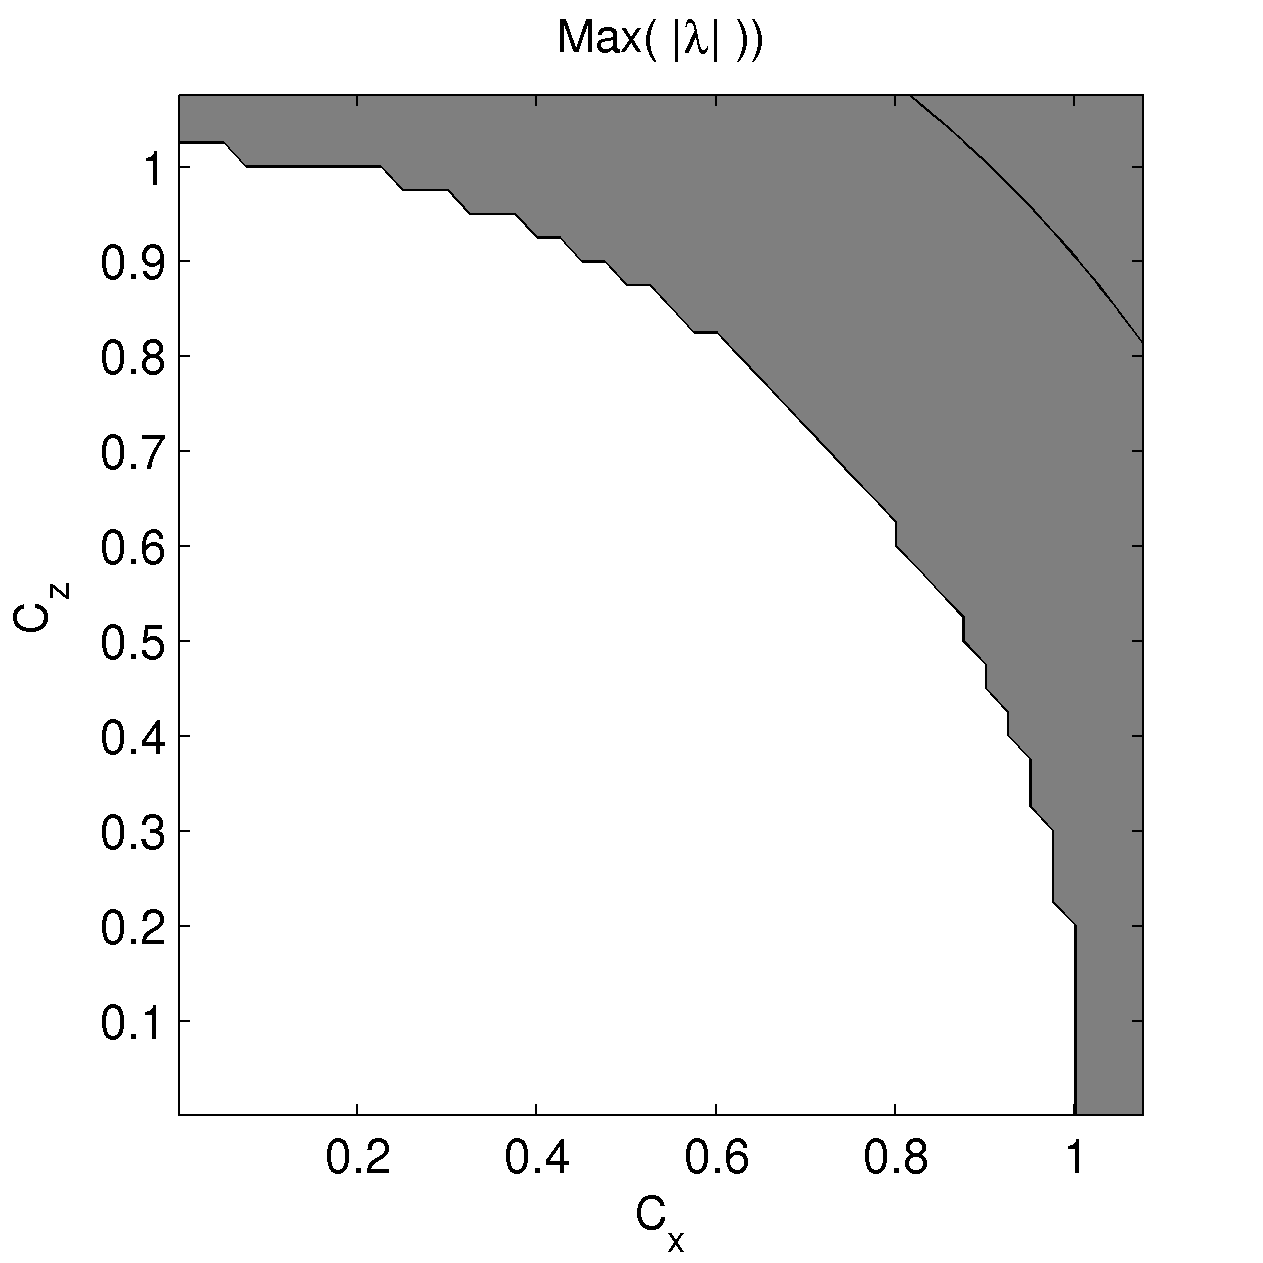
\includegraphics[width=.4\textwidth]{FIGURES/stabcs2.png}}\quad
   \subfloat[][]{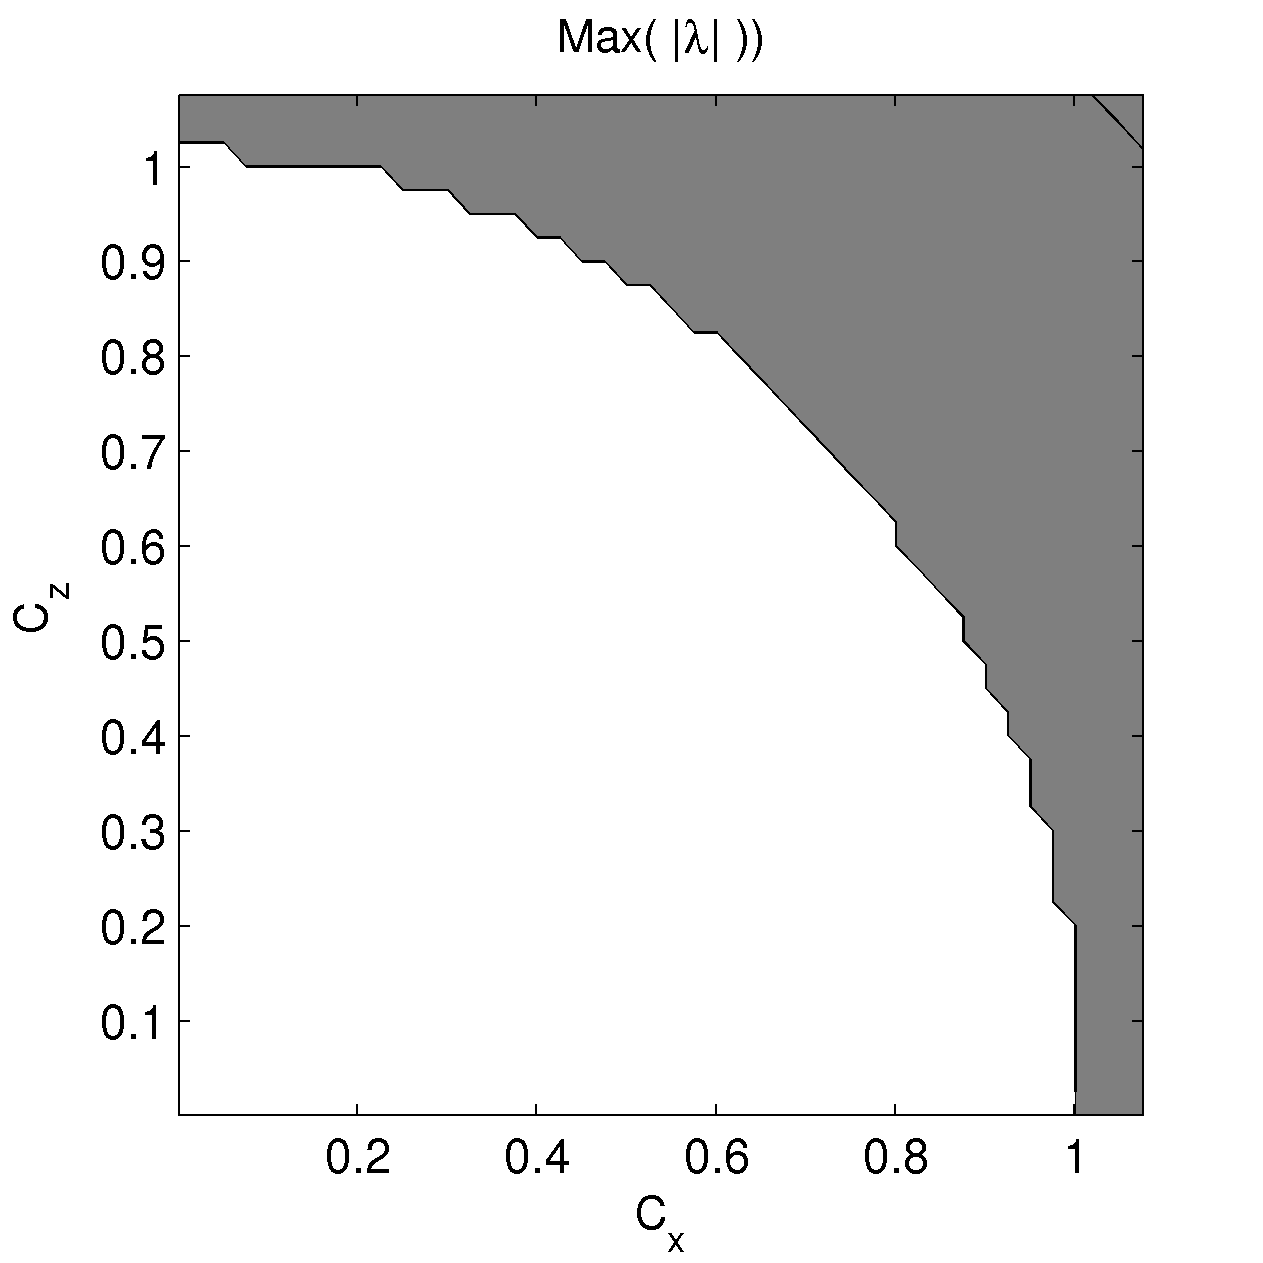
\includegraphics[width=.4\textwidth]{FIGURES/stabcs10.png}}\\
   \subfloat[][]{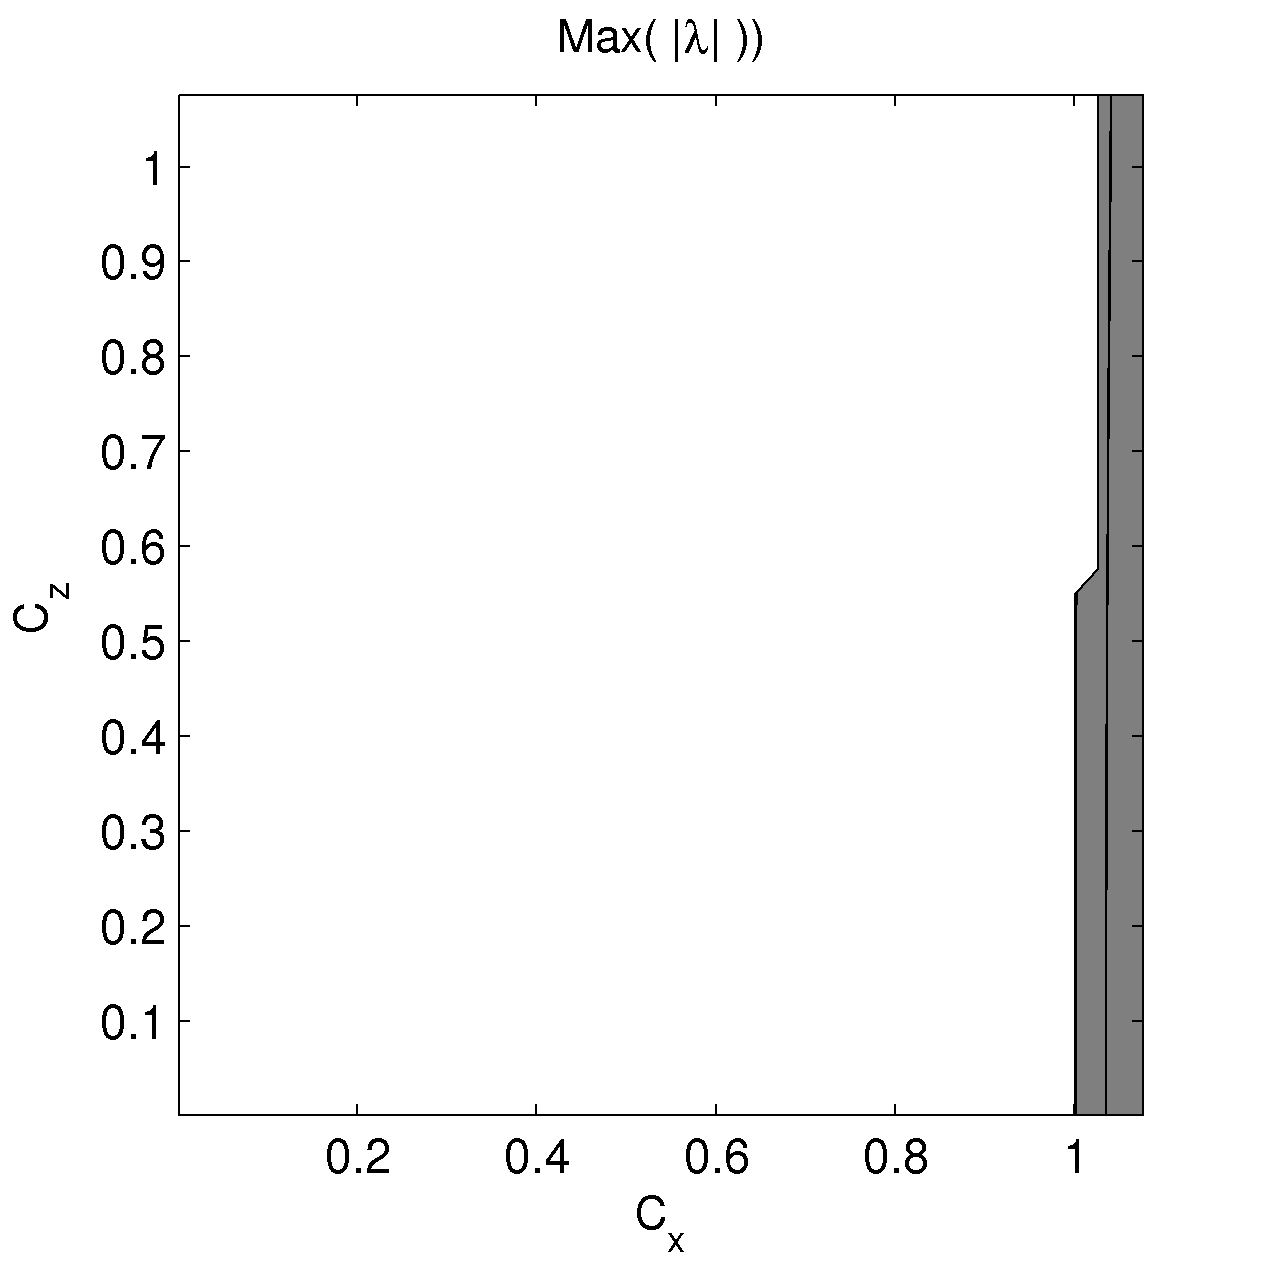
\includegraphics[width=.4\textwidth]{FIGURES/stabcs2imp.png}}\quad
   \subfloat[][]{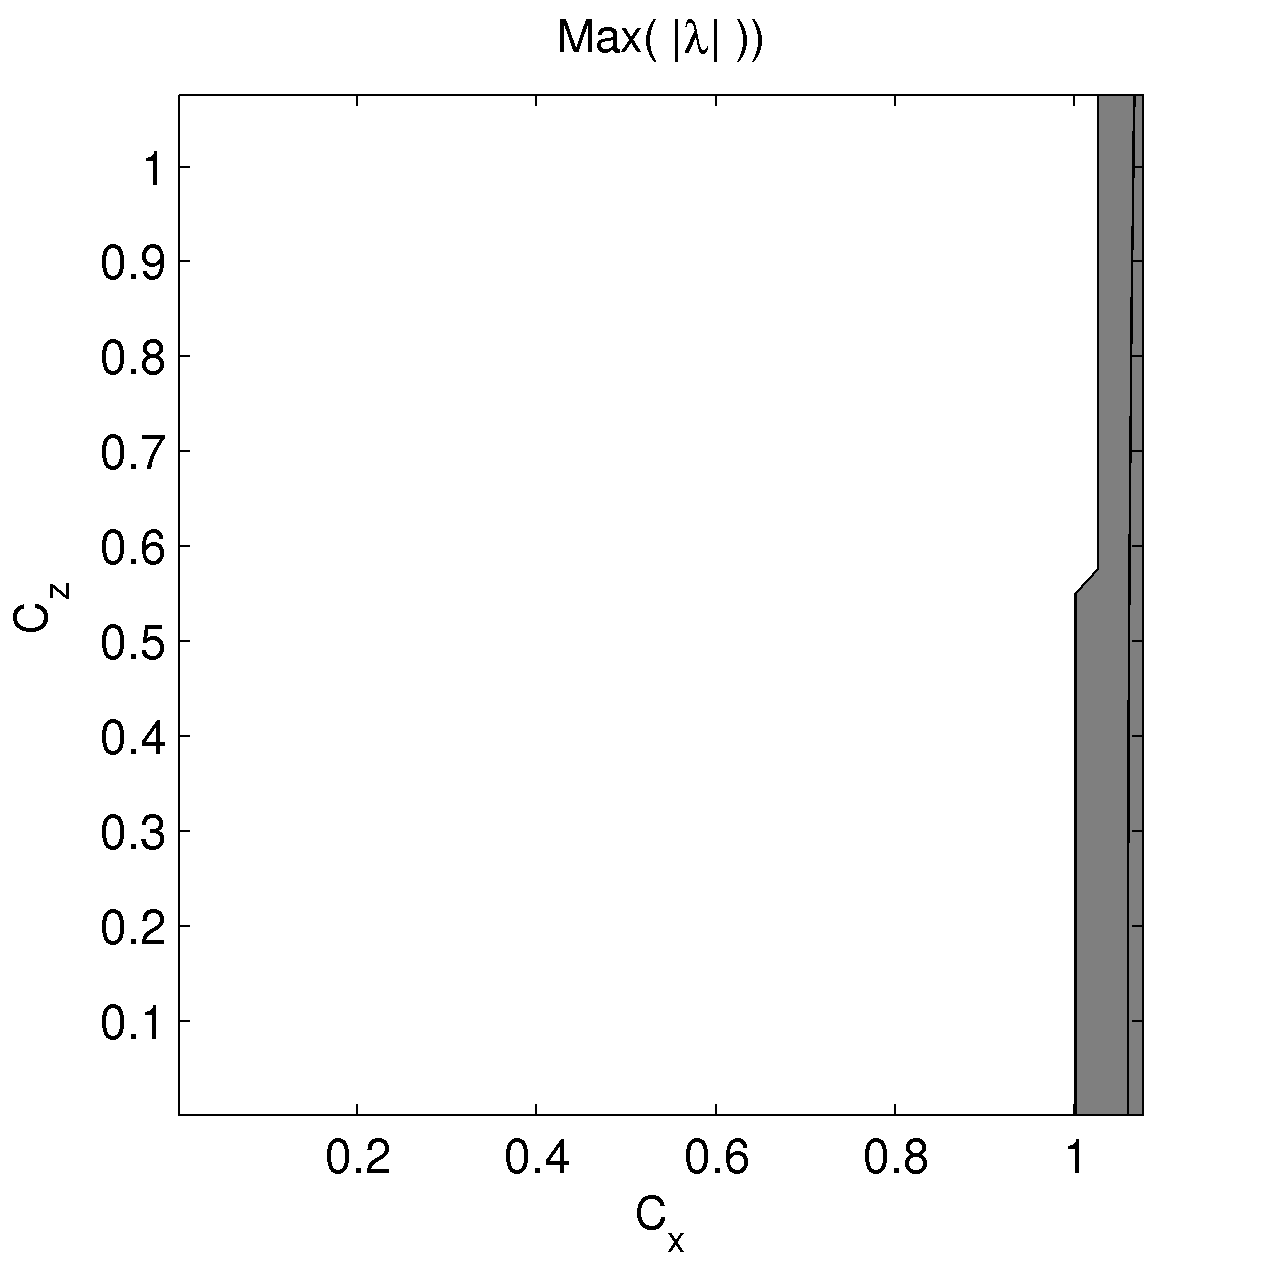
\includegraphics[width=.4\textwidth]{FIGURES/stabcs10imp.png}}\\
   %\subfloat[][]{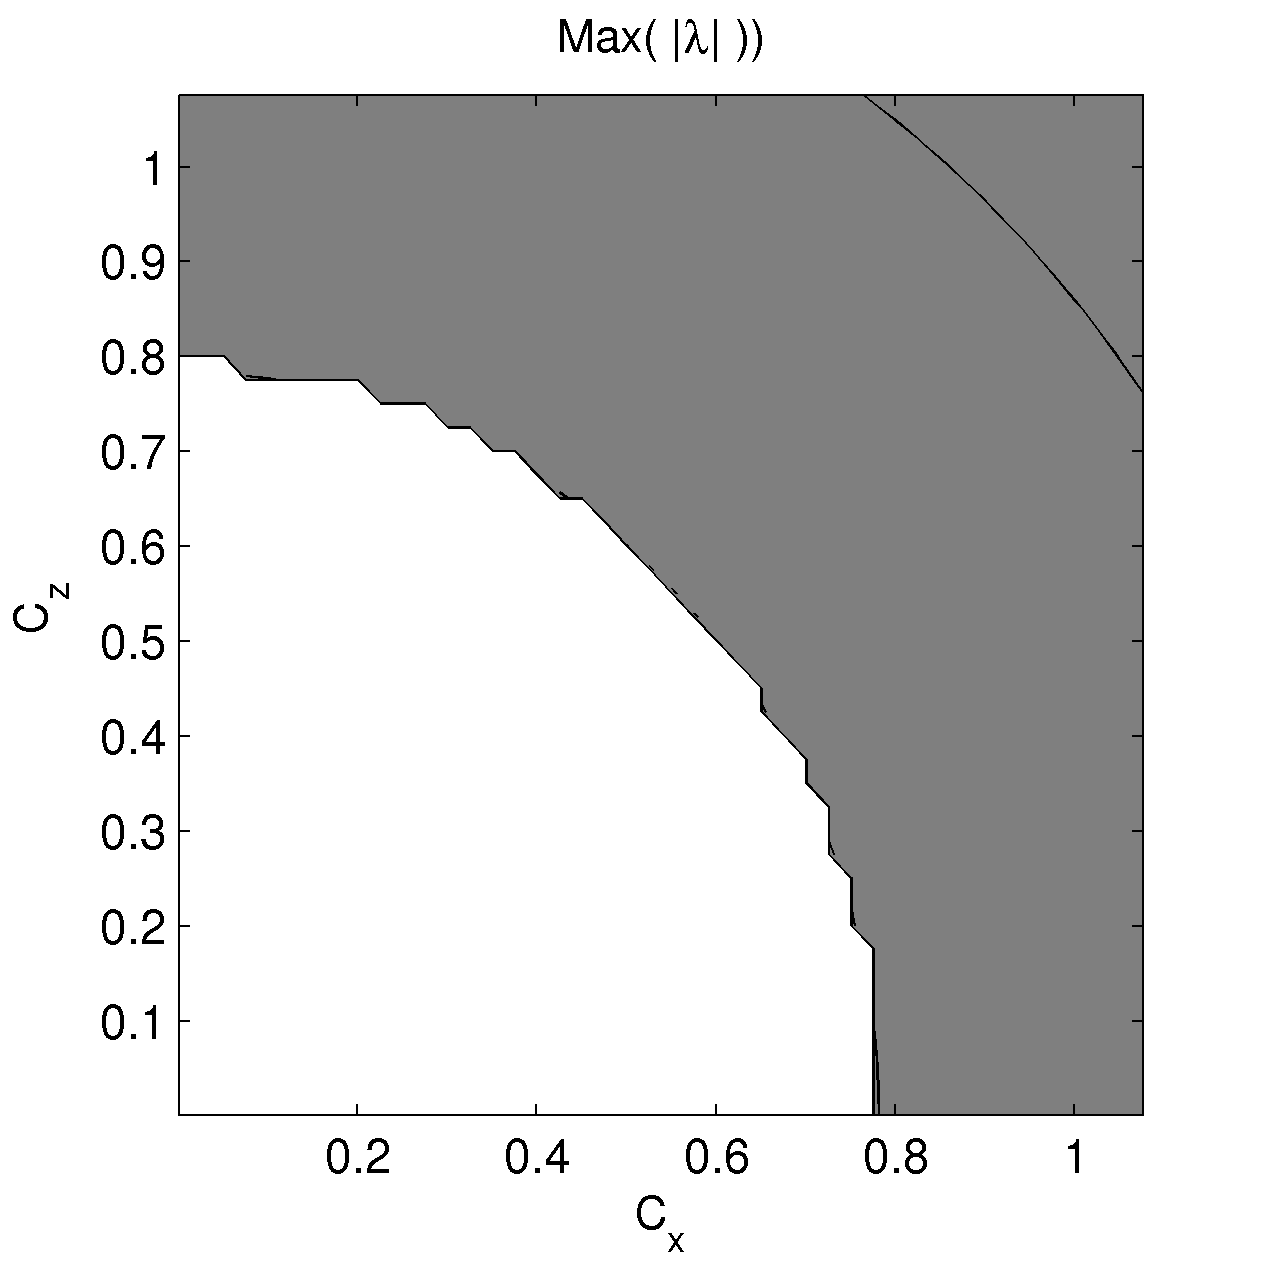
\includegraphics[width=.4\textwidth]{FIGURES/stabcs2lambda.png}}\quad
   %\subfloat[][]{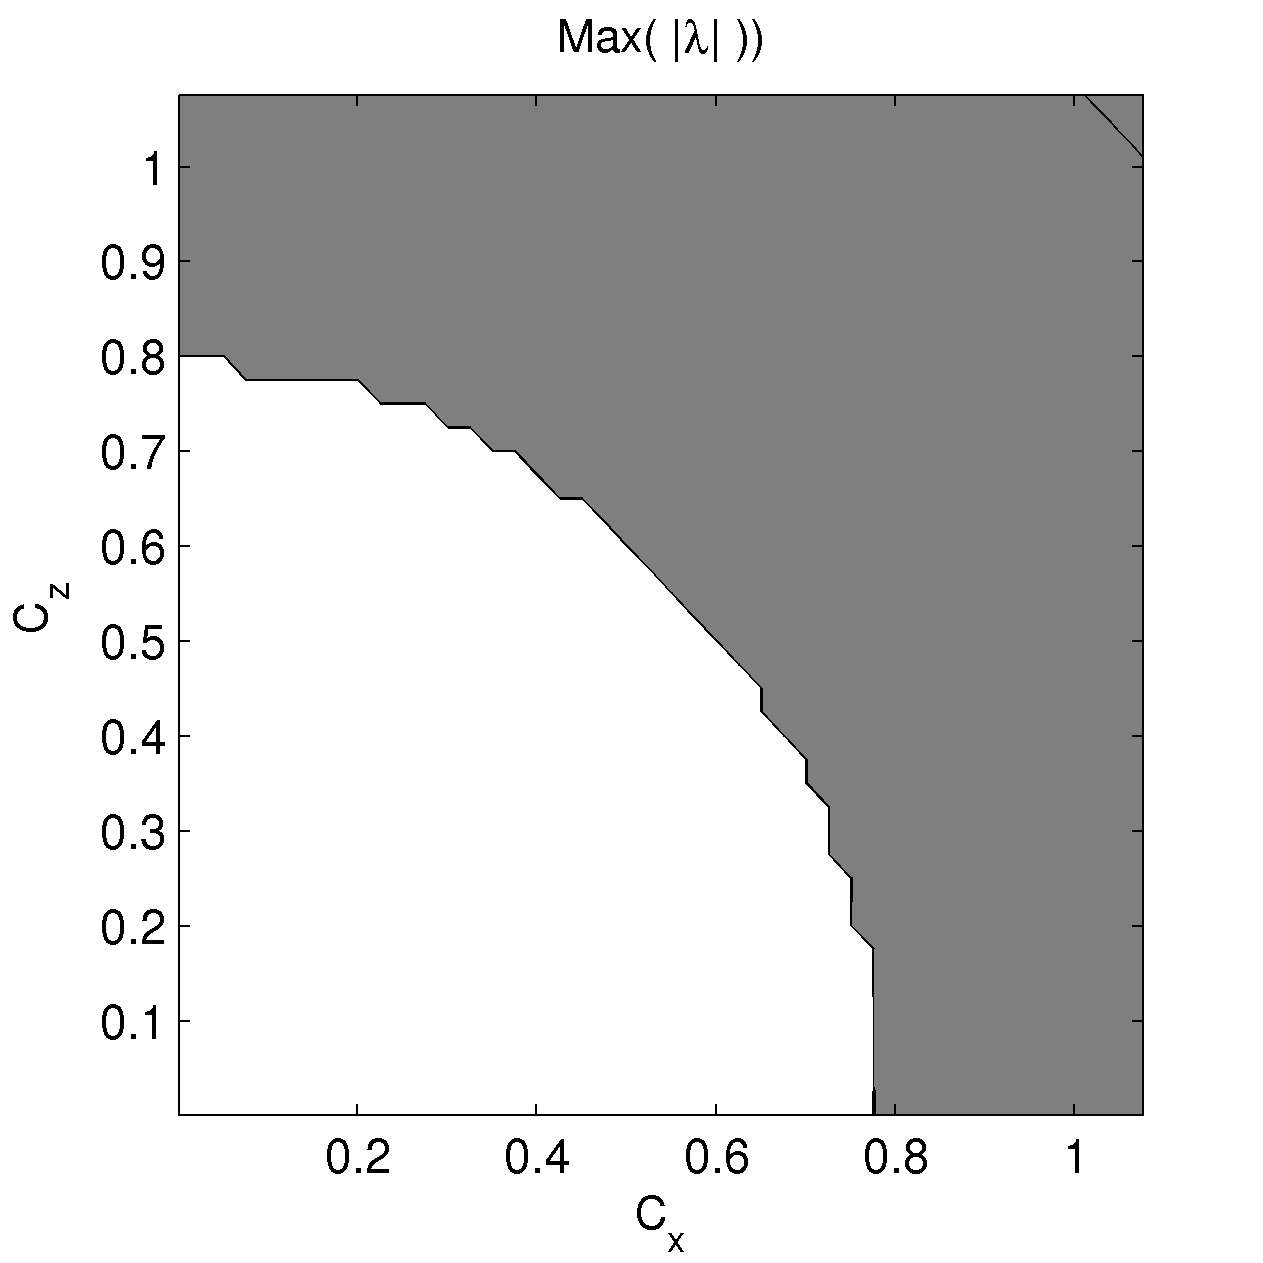
\includegraphics[width=.4\textwidth]{FIGURES/stabcs10lambda.png}}
   \caption {Amplitude of the largest eigenvalue as a function of $C_x\ =\ C_z$ and $C_\lambda$.\\
   Unstable area ($\mid\lambda\mid >1$) is in grey. }
   \label{Figstabcs}
\end{figure}

\begin{figure}[!ht]
   \centering
   \subfloat[][]{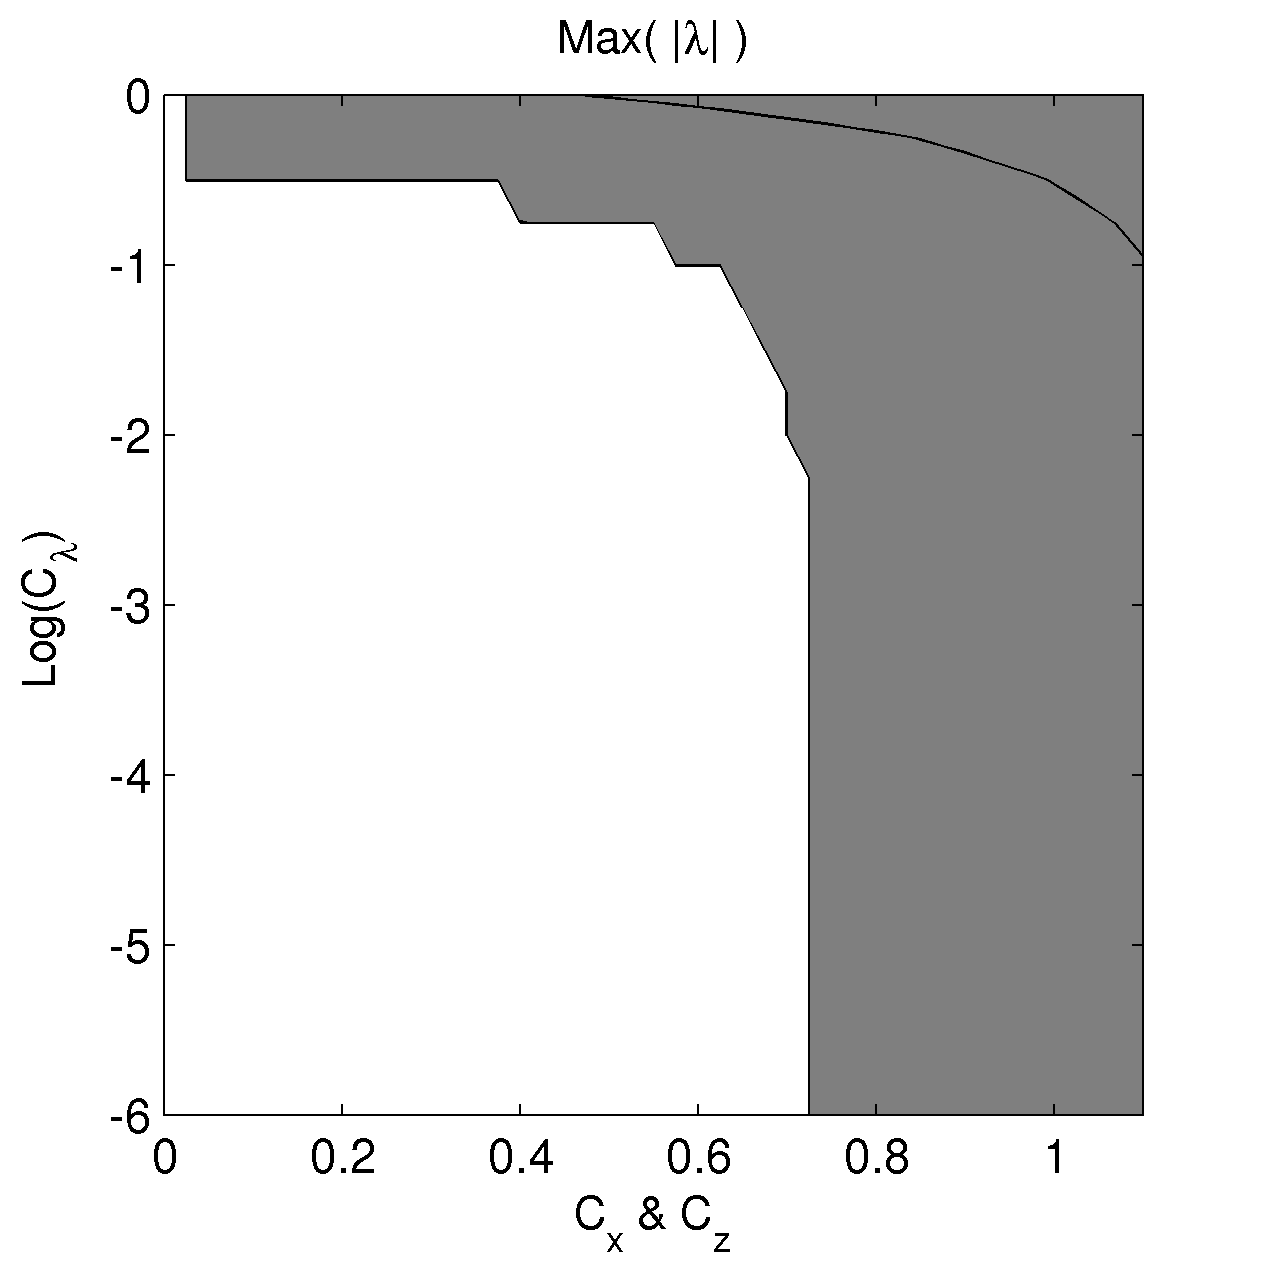
\includegraphics[width=.4\textwidth]{FIGURES/stablambda_cpl2.png}}\quad
   \subfloat[][]{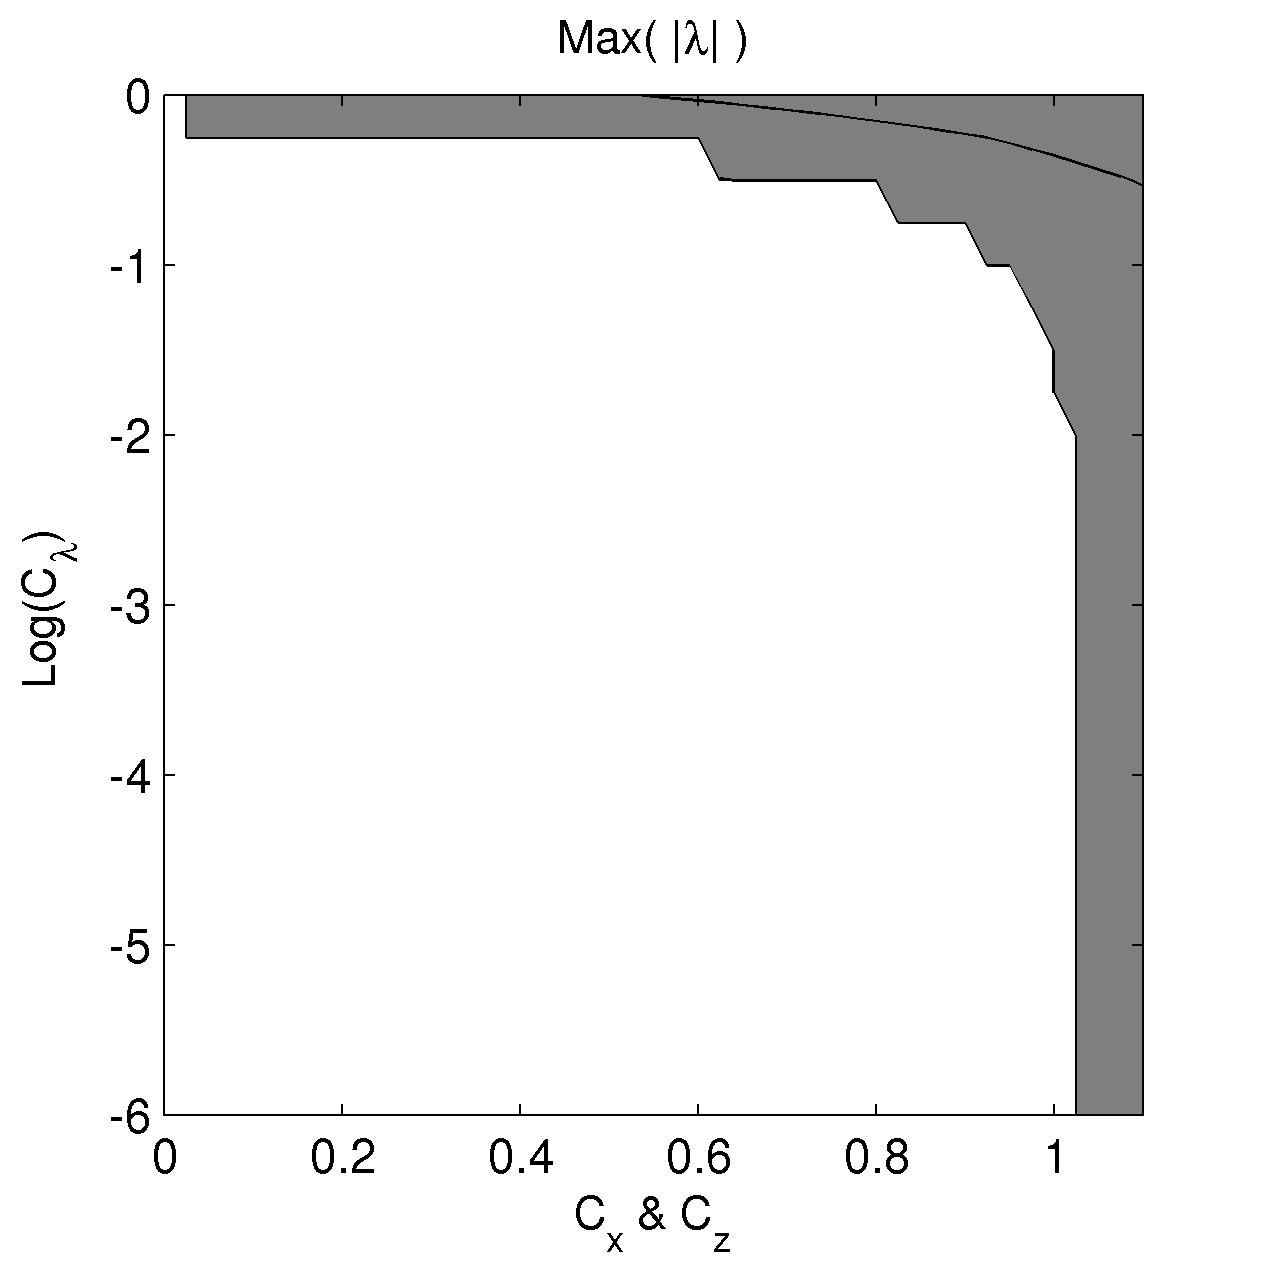
\includegraphics[width=.4\textwidth]{FIGURES/stablambdaimp_cpl2.png}}
   \caption {Amplitude of the largest eigenvalue as a function of $C_x\ =\ C_z$ and $C_\lambda$.\\
   Unstable area ($\mid\lambda\mid >1$) is in grey.\\
   (a): FB scheme, (b): FBi scheme. }
   \label{Figstabcslambda}
\end{figure}

\begin{figure}[!ht]
   \centering
   \subfloat[][]{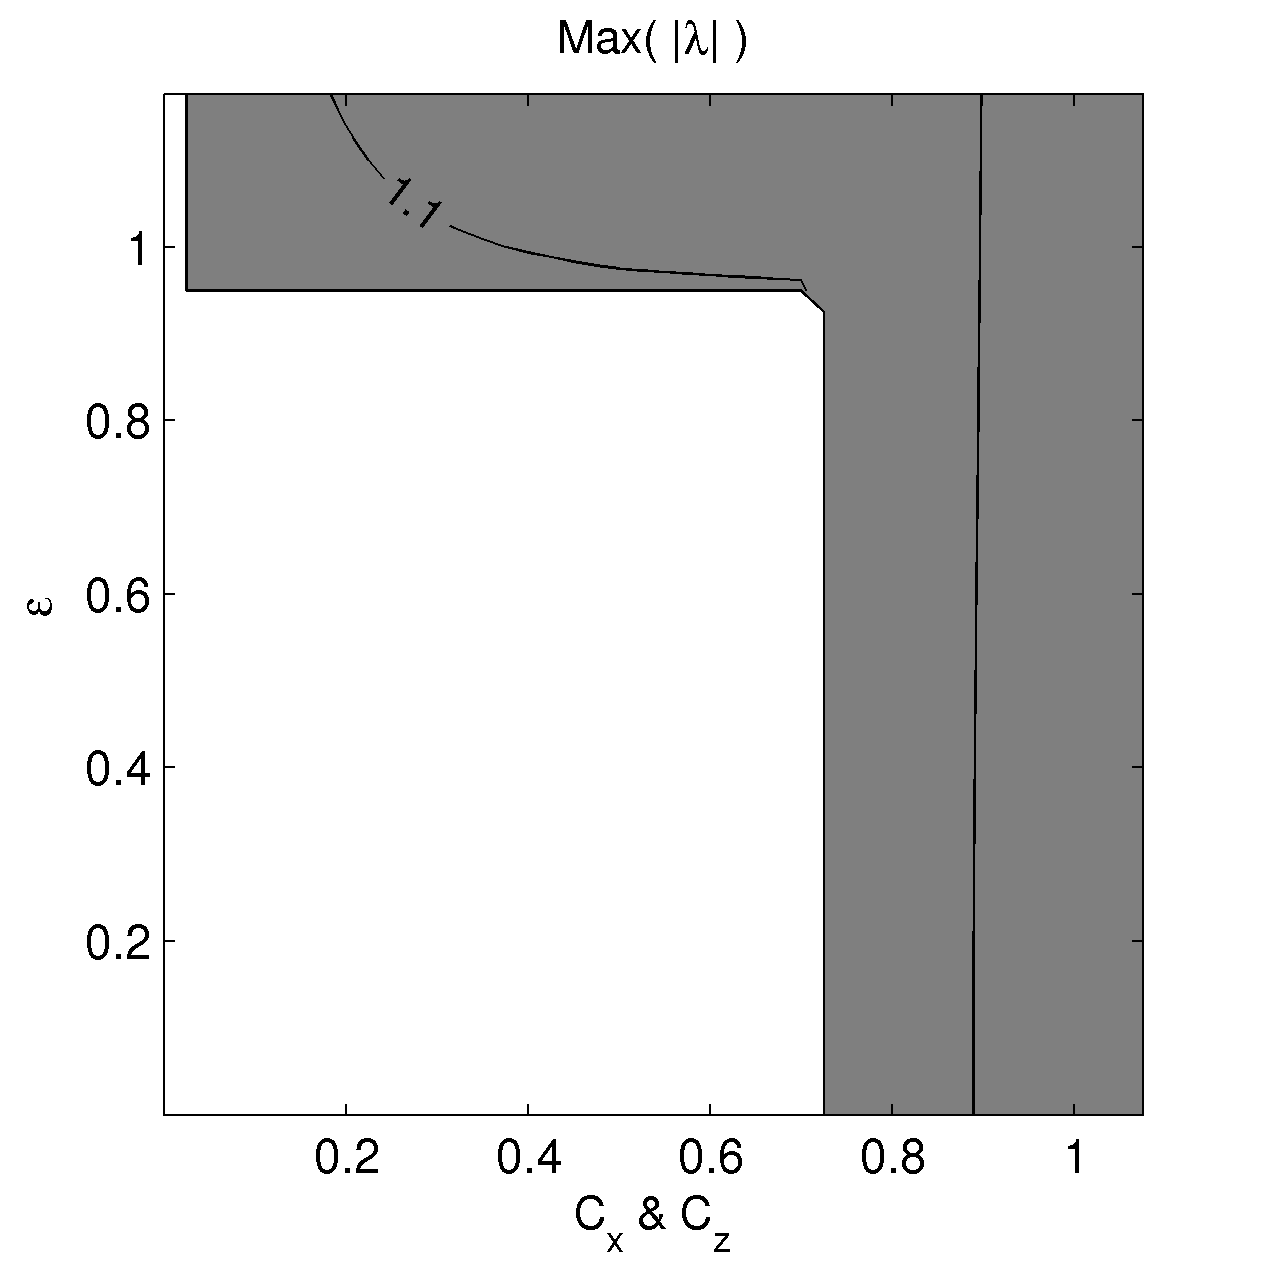
\includegraphics[width=.4\textwidth]{FIGURES/stabsurf.png}}\quad
   \subfloat[][]{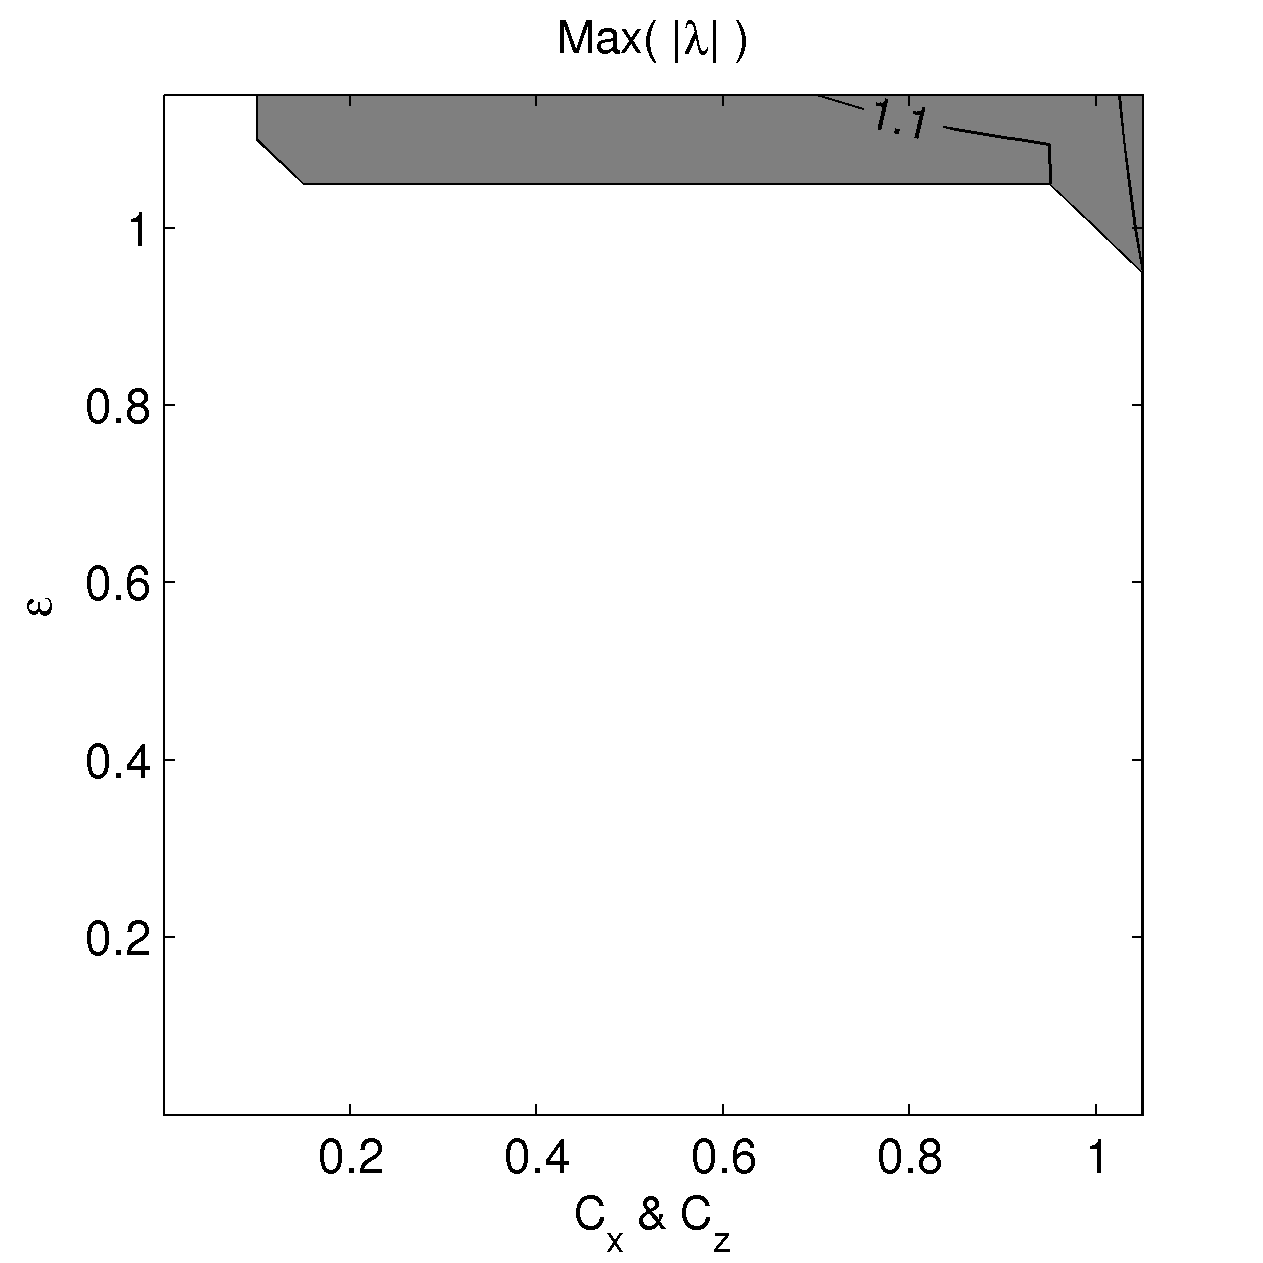
\includegraphics[width=.4\textwidth]{FIGURES/stabsurfimp.png}}
   \caption {Amplitude of the largest eigenvalue as a function of $C_x\ =\ C_z$ and $\epsilon$.\\
   Unstable area ($\mid\lambda\mid >1$) is in grey.\\
   (a): FB scheme, (b): FBi scheme. }
   \label{Figstabsurf}
\end{figure}

\begin{figure}[!ht]
   \centering
   \subfloat[][]{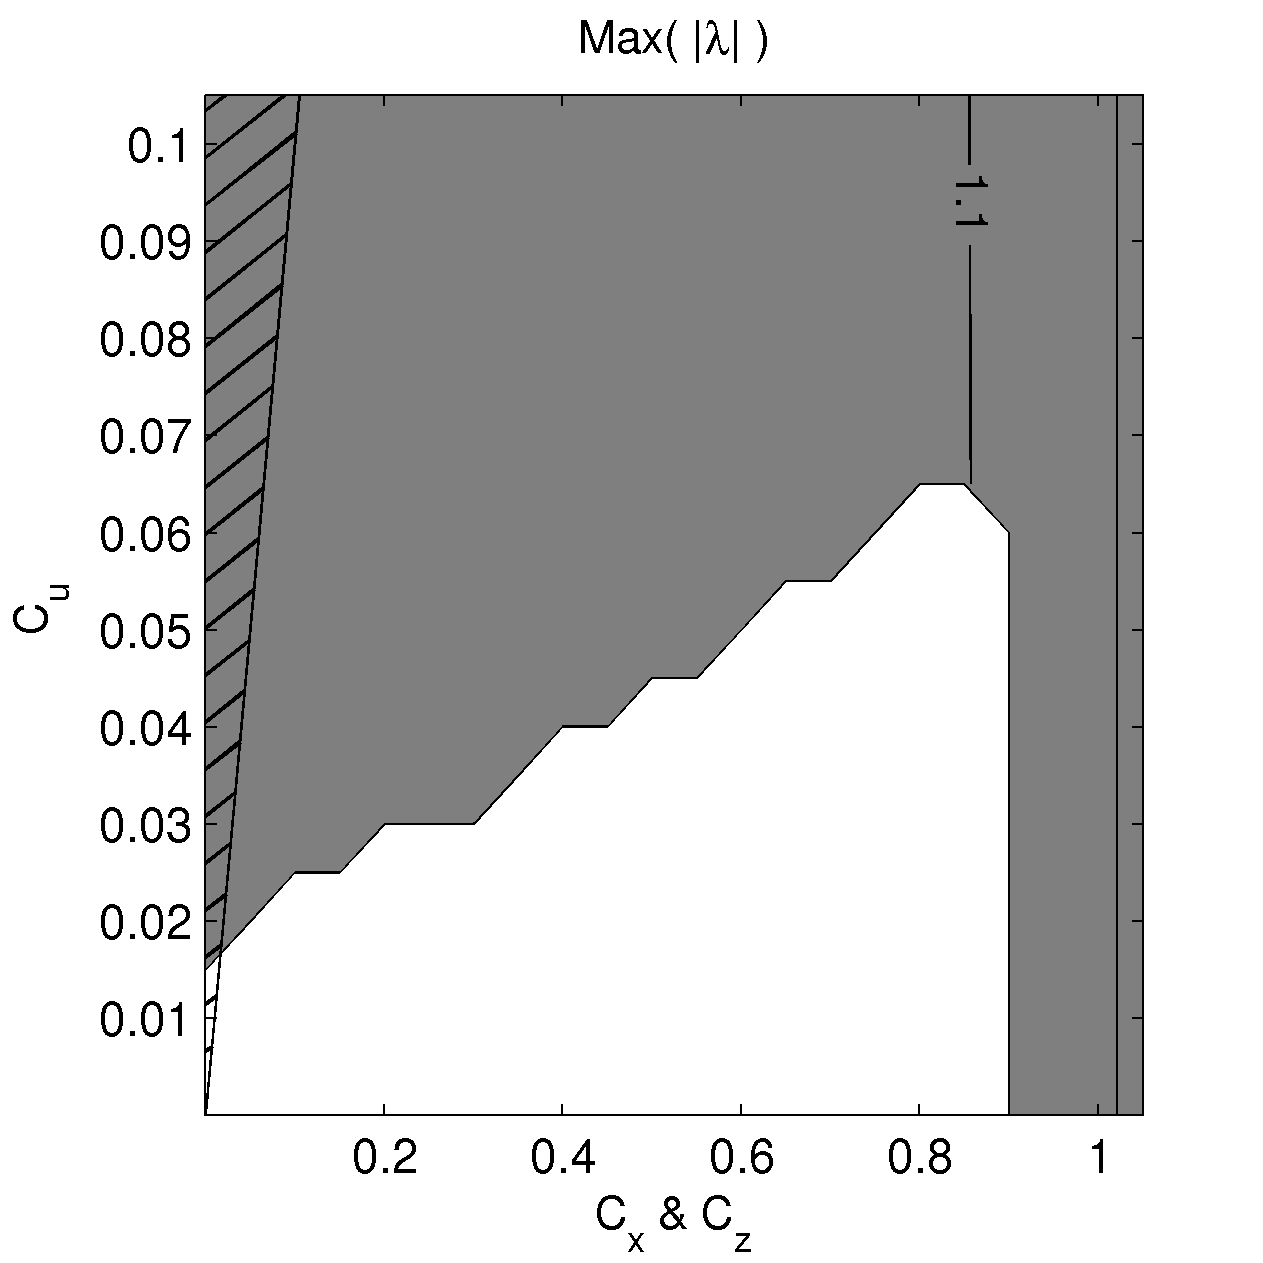
\includegraphics[width=.4\textwidth]{FIGURES/stabadv_cplA.png}}\quad
   \subfloat[][]{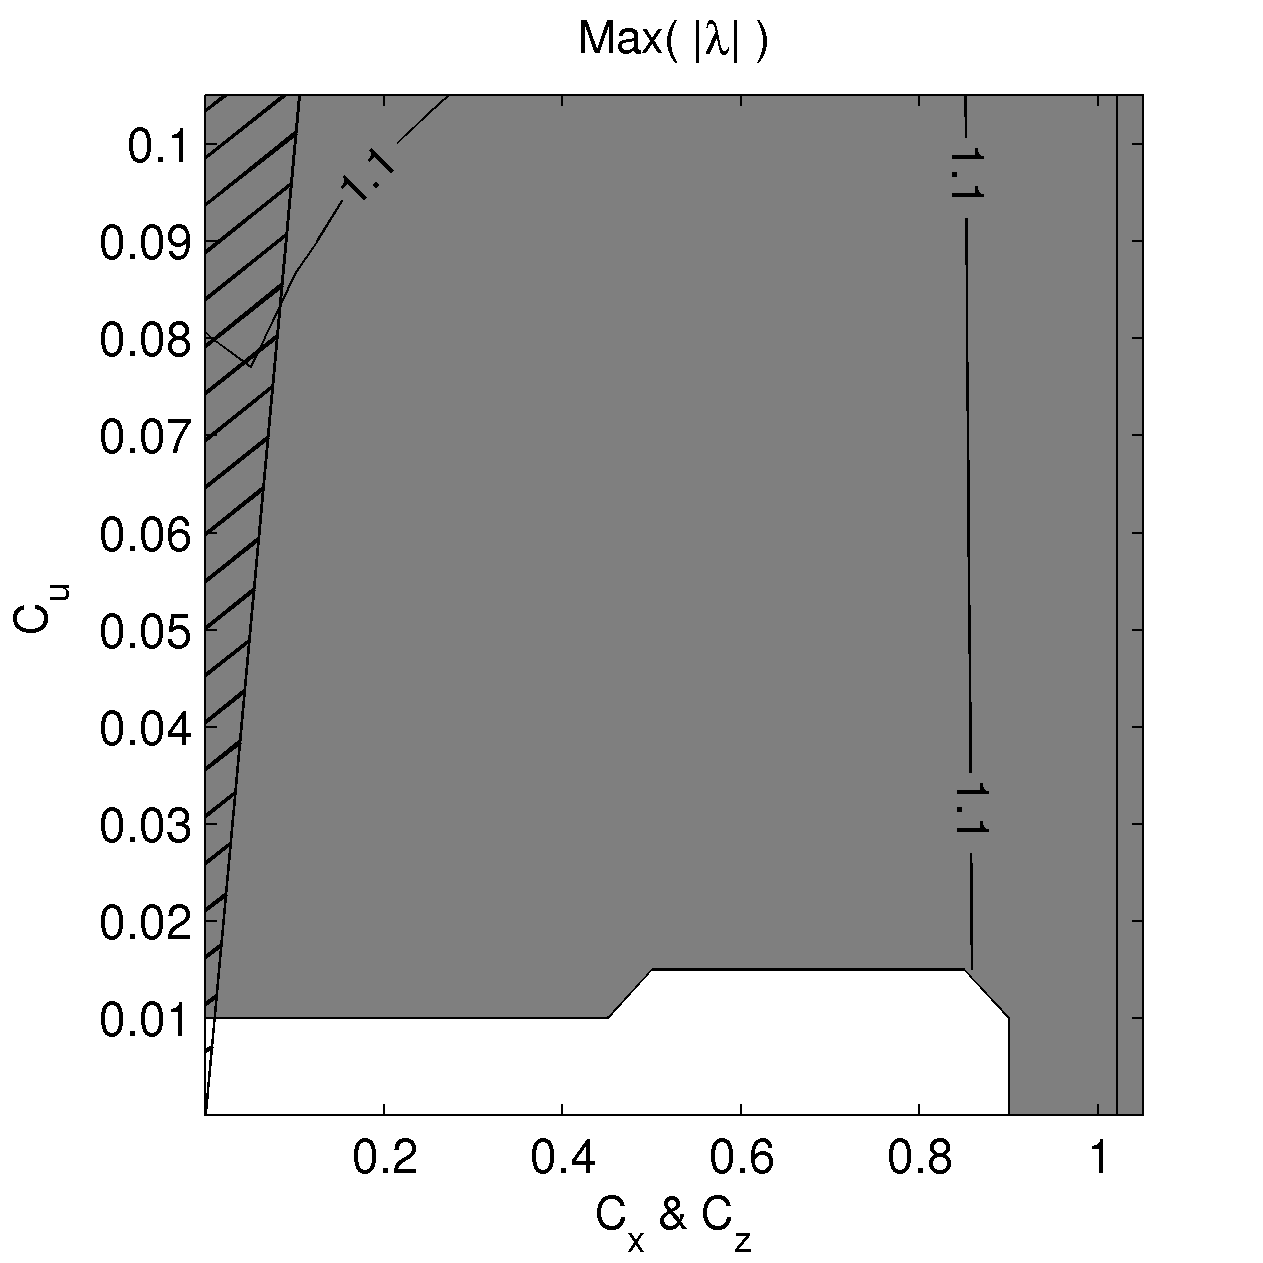
\includegraphics[width=.4\textwidth]{FIGURES/stabadv_cplB.png}}\\
   \subfloat[][]{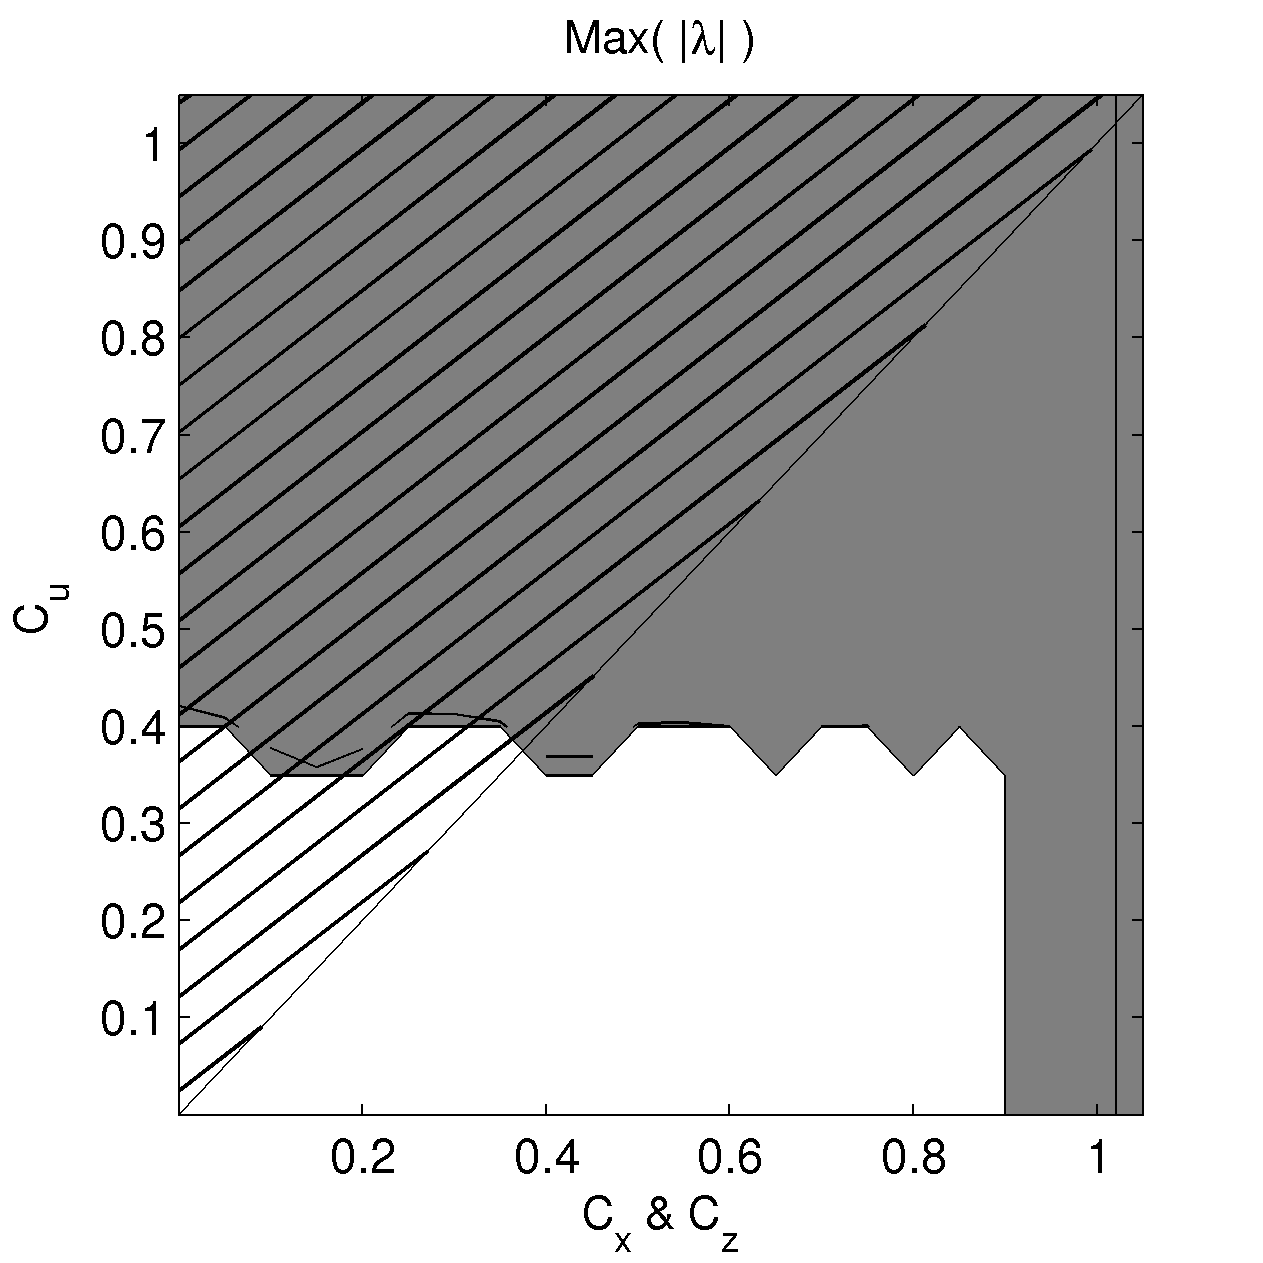
\includegraphics[width=.4\textwidth]{FIGURES/stabadv_cplBi.png}}\quad
   \subfloat[][]{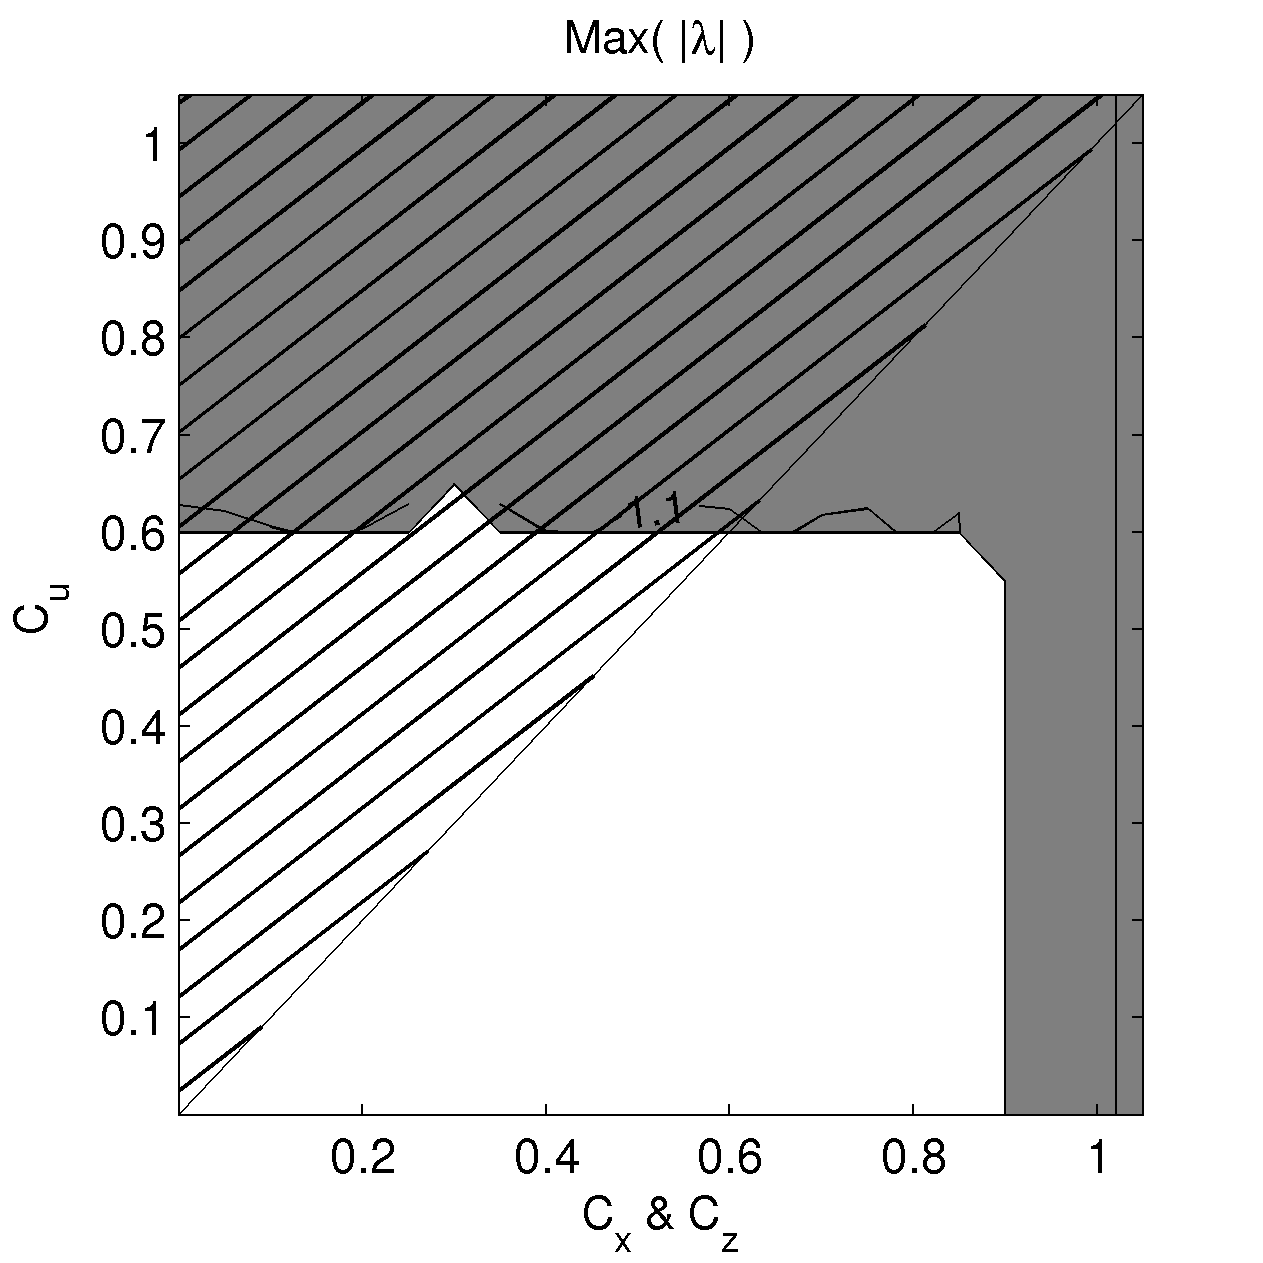
\includegraphics[width=.4\textwidth]{FIGURES/stabadvlambdaimp10_cpl2.png}}
   \caption{Amplitude of the largest eigenvalue as a function of $C_x\ =\ C_z$ and $C_u$.\\
       Unstable area ($\mid\lambda\mid >1$) is in grey.\\
       Hatched area: $C_u > C_x$ \\
       (a): Scheme Cpl-A. (b): Scheme Cpl-B.\\
       (c): Scheme Cpl-Bi. (d): Scheme Cpl-C.\\
       (a) and (b): vertical range has been divided by 10.}
   \label{Figstabadvsch}
\end{figure}

\begin{figure}[!ht]
   \centering
   \subfloat[][]{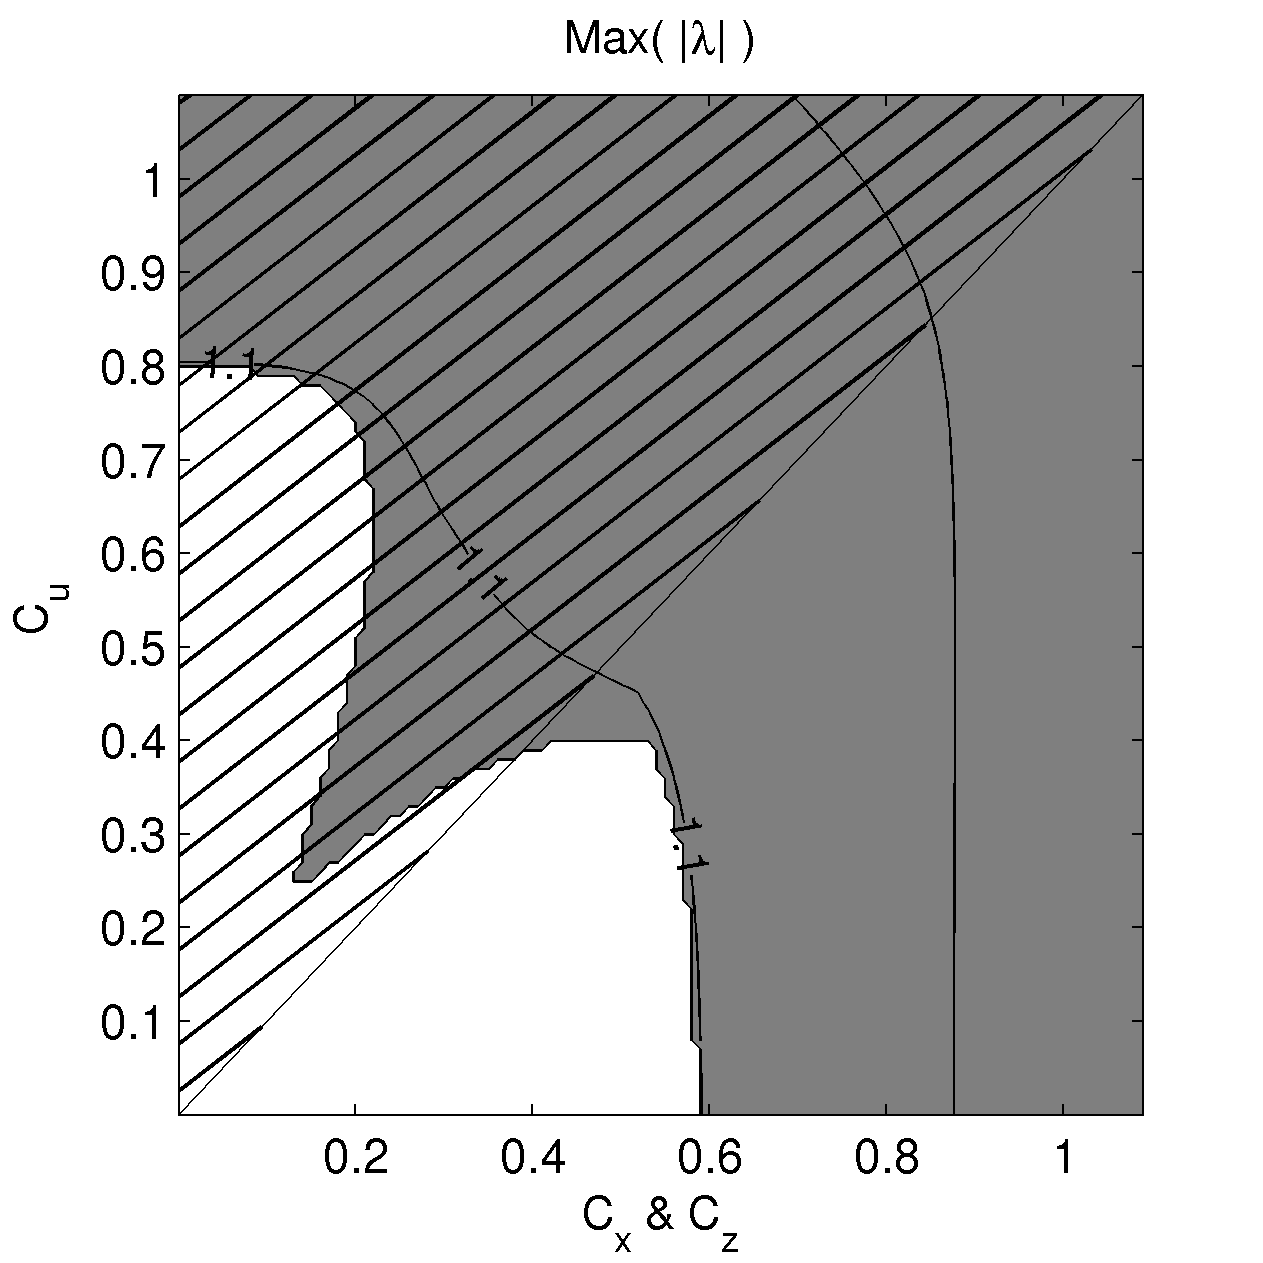
\includegraphics[width=.4\textwidth]{FIGURES/stabadv1_cpl2.png}}\quad
   \subfloat[][]{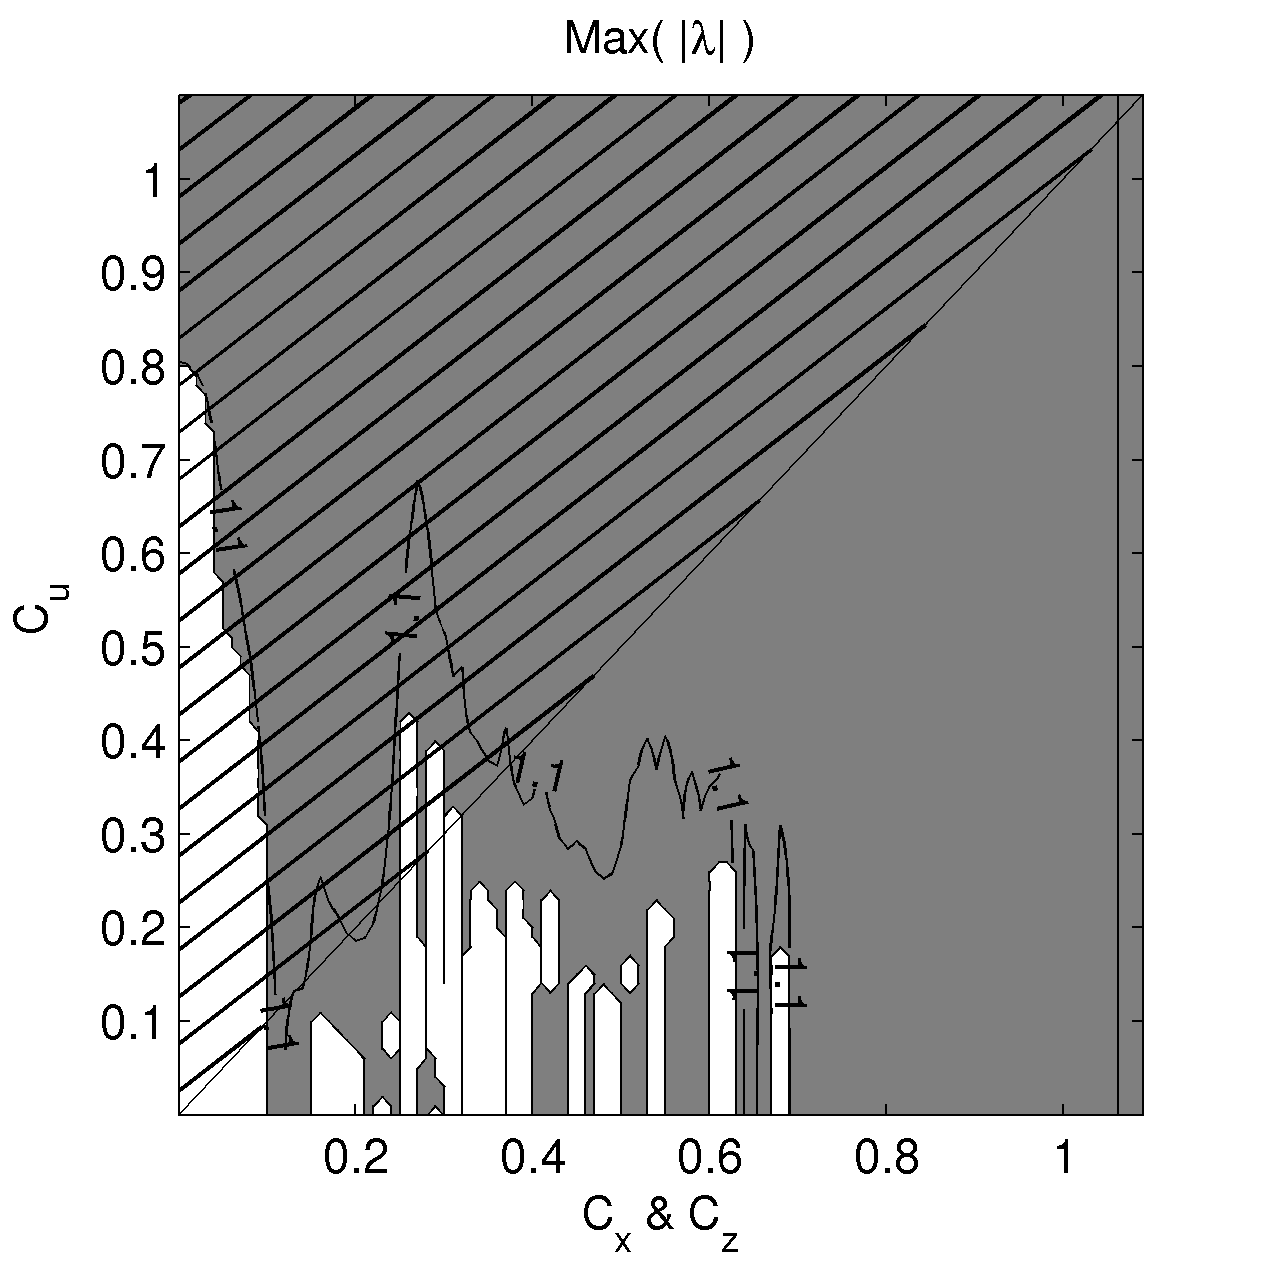
\includegraphics[width=.4\textwidth]{FIGURES/stabadv10_cpl2.png}}\\
   \subfloat[][]{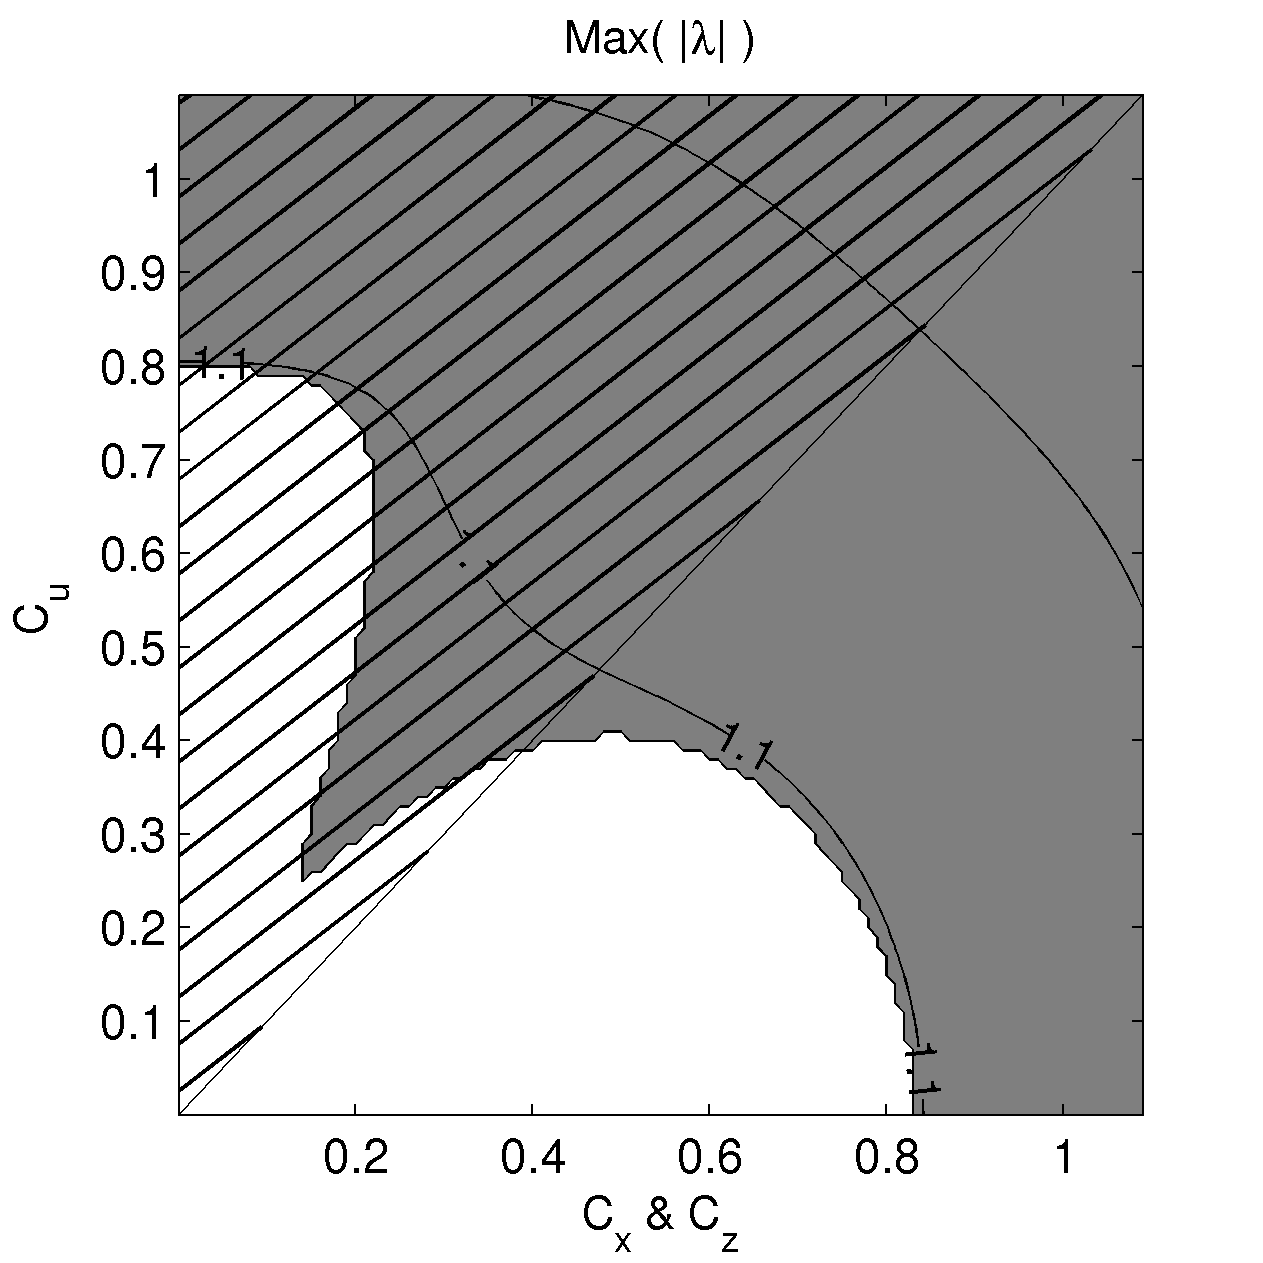
\includegraphics[width=.4\textwidth]{FIGURES/stabadvimp1_cpl2.png}}\quad
   \subfloat[][]{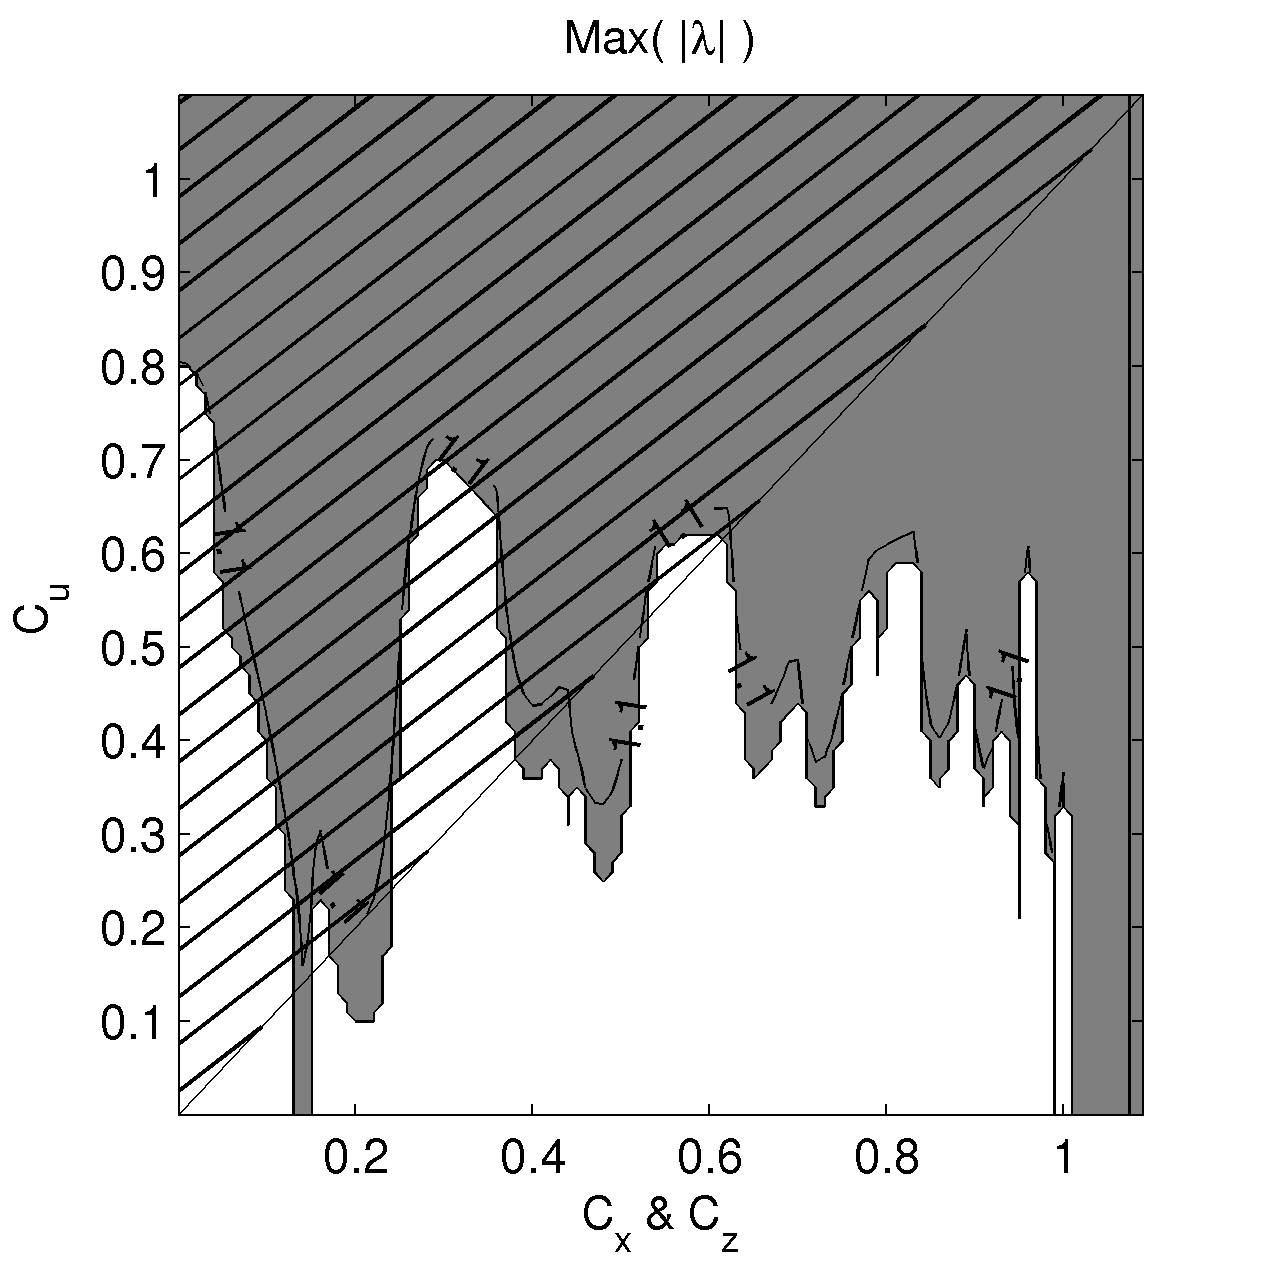
\includegraphics[width=.4\textwidth]{FIGURES/stabadvimp10_cpl2.png}}\\
   \subfloat[][]{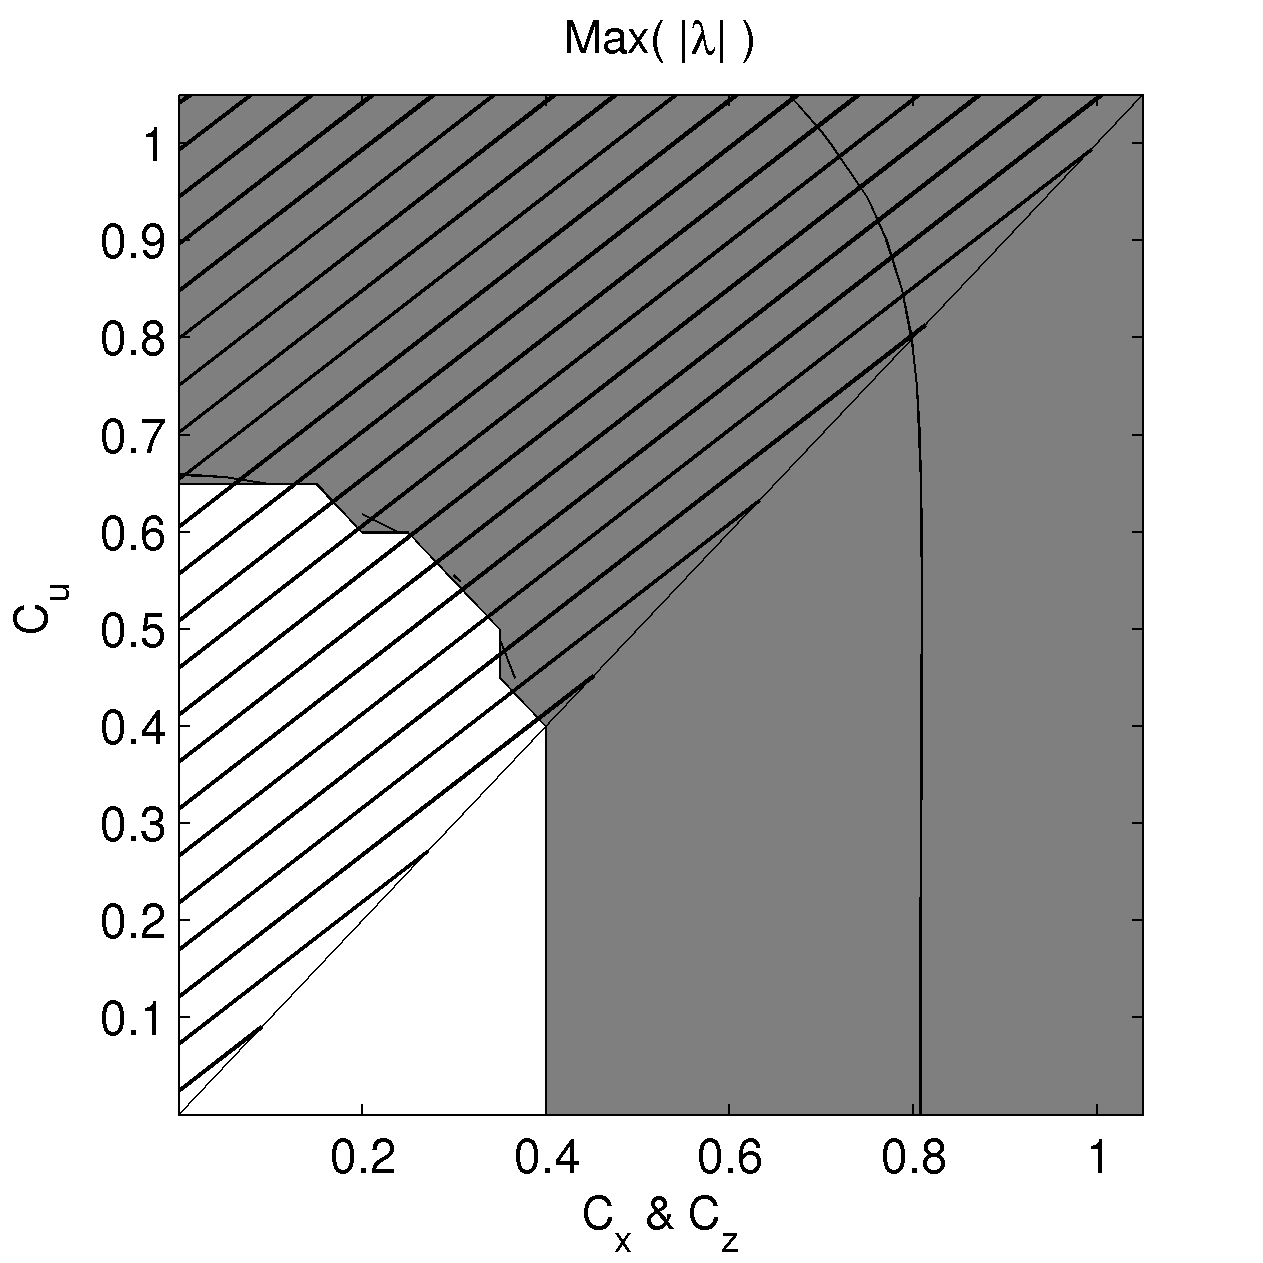
\includegraphics[width=.4\textwidth]{FIGURES/stabadvlambda1_cpl2.png}}\quad
   \subfloat[][]{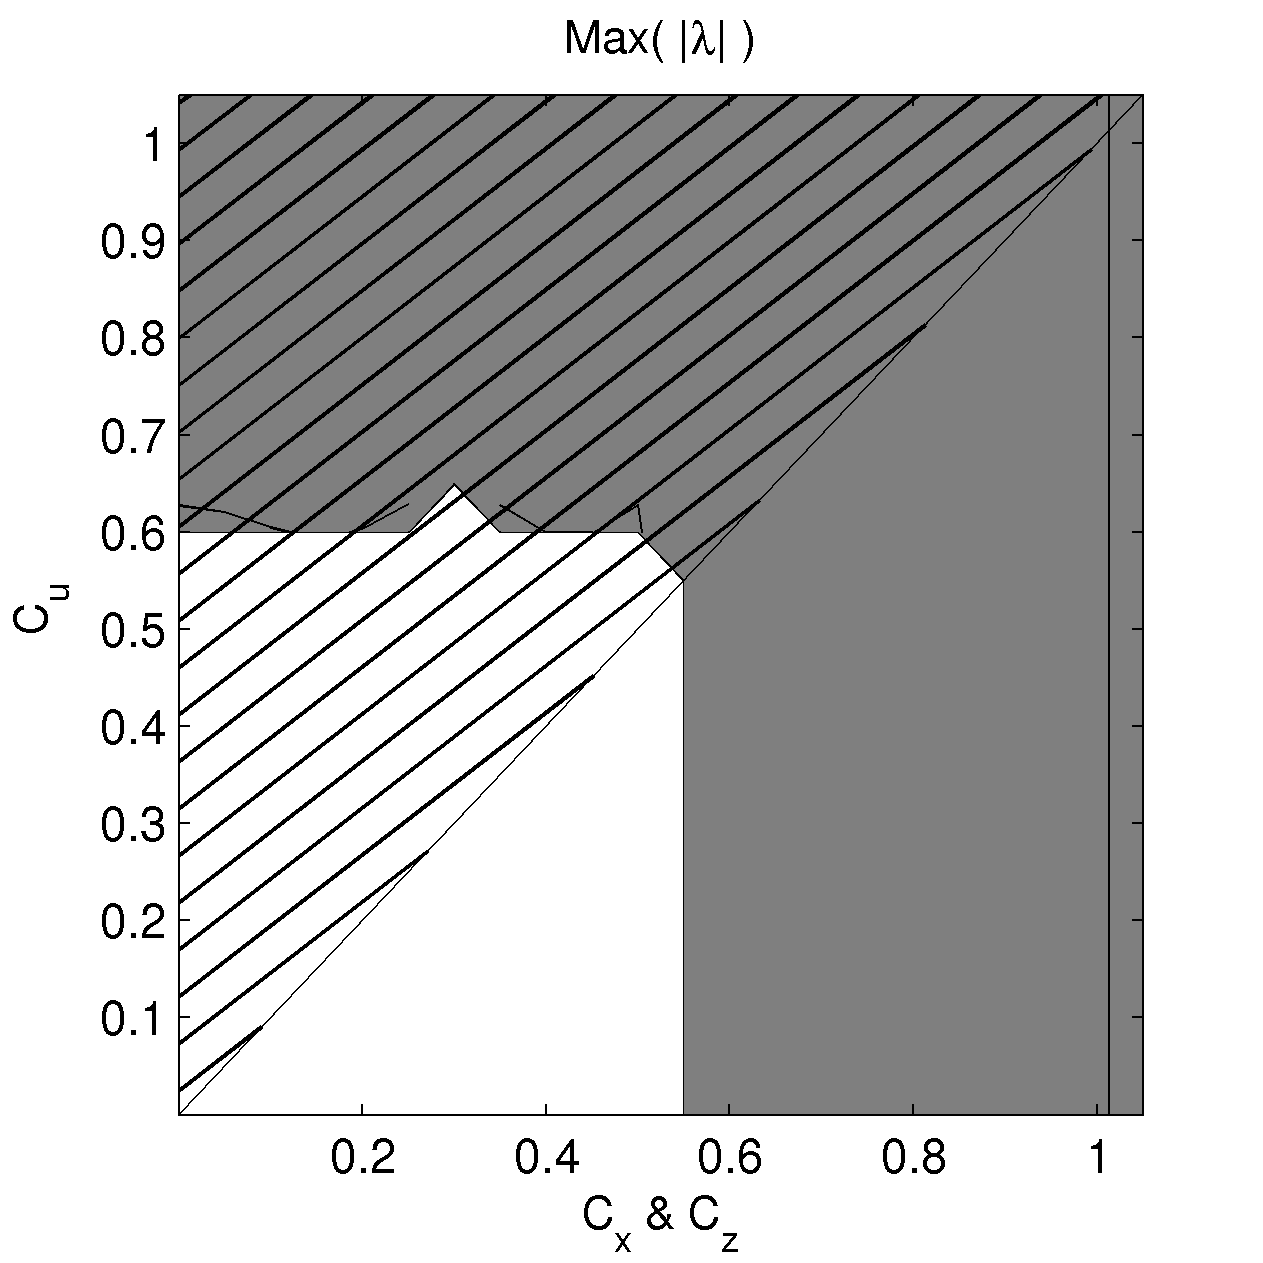
\includegraphics[width=.4\textwidth]{FIGURES/stabadvlambda10_cpl2.png}}
   \caption{Amplitude of the largest eigenvalue as a function of $C_x\ =\ C_z$ and $C_u$.\\
       Unstable area ($\mid\lambda\mid >1$) is in grey.\\
       Hatched area: $C_u > C_x$ \\
       (a), (c), (e): $N_f = 1$. (b), (d), (f): $N_f = 10$.\\
       (a) and (b): reference FB scheme.\\
       (c) and (d): w-implicit FB scheme.\\
       (e) and (f): reference FB scheme with $\lambda_s = 0.1\ m^2/s$.}
   \label{Figstabadv}
\end{figure}


%\begin{figure}[!ht]
%   \centering
%   \subfloat[][]{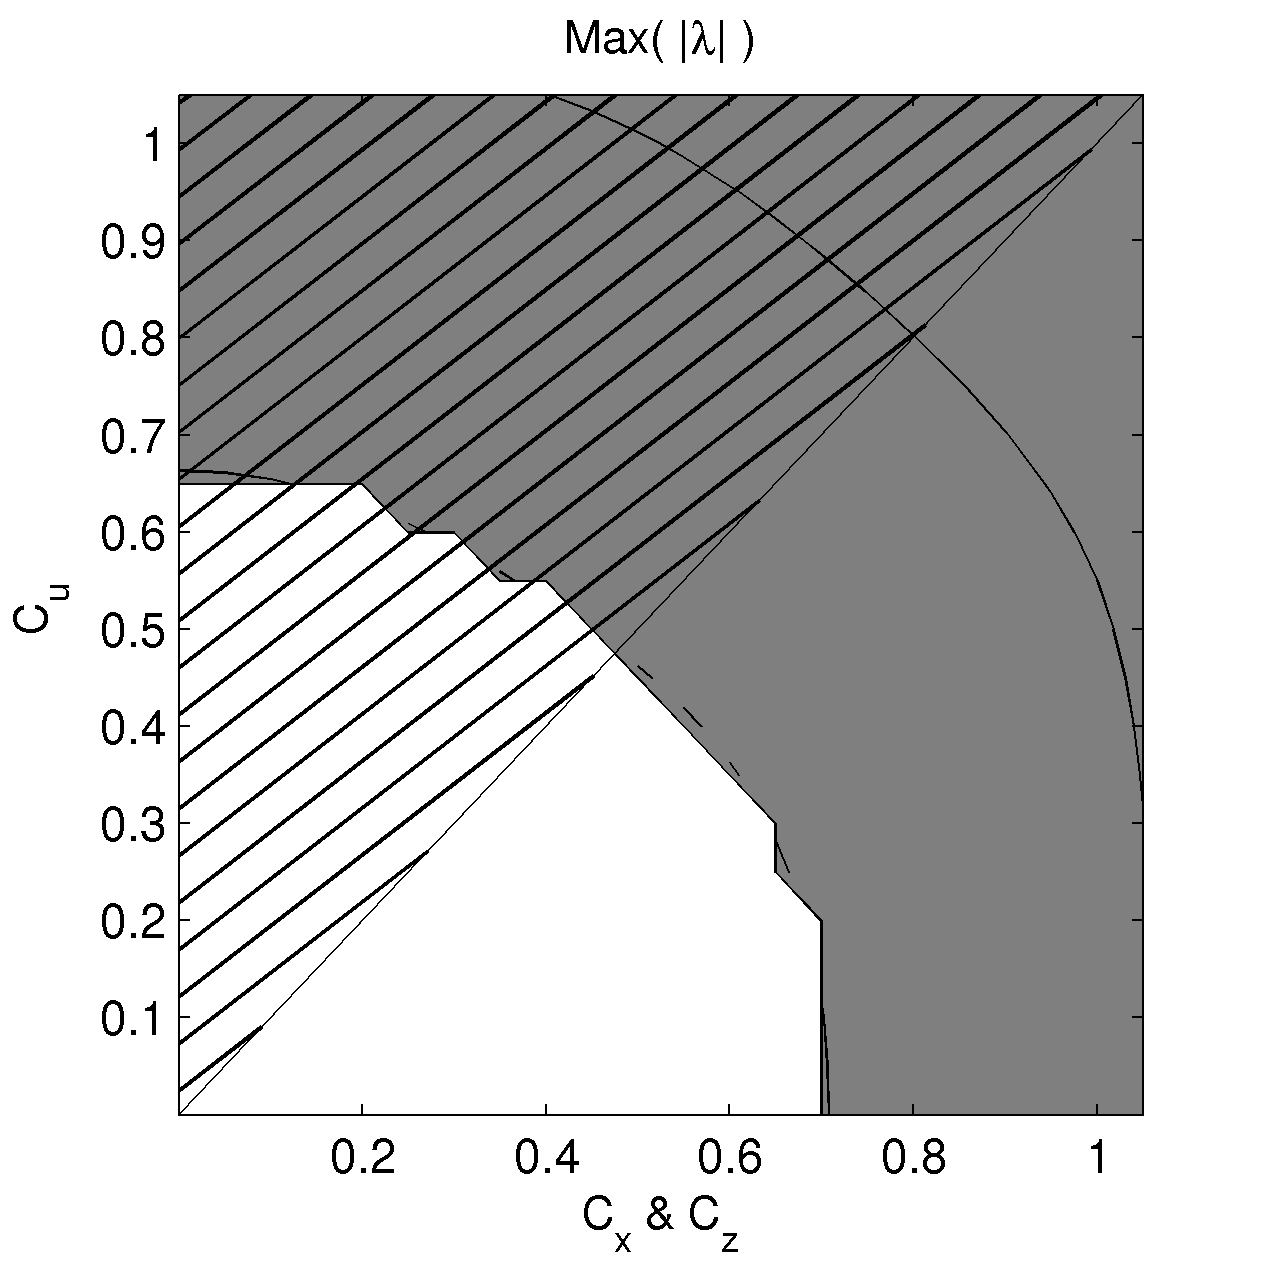
\includegraphics[width=.4\textwidth]{FIGURES/stabadvlambdaimp1_cpl2.png}}\quad
%   \subfloat[][]{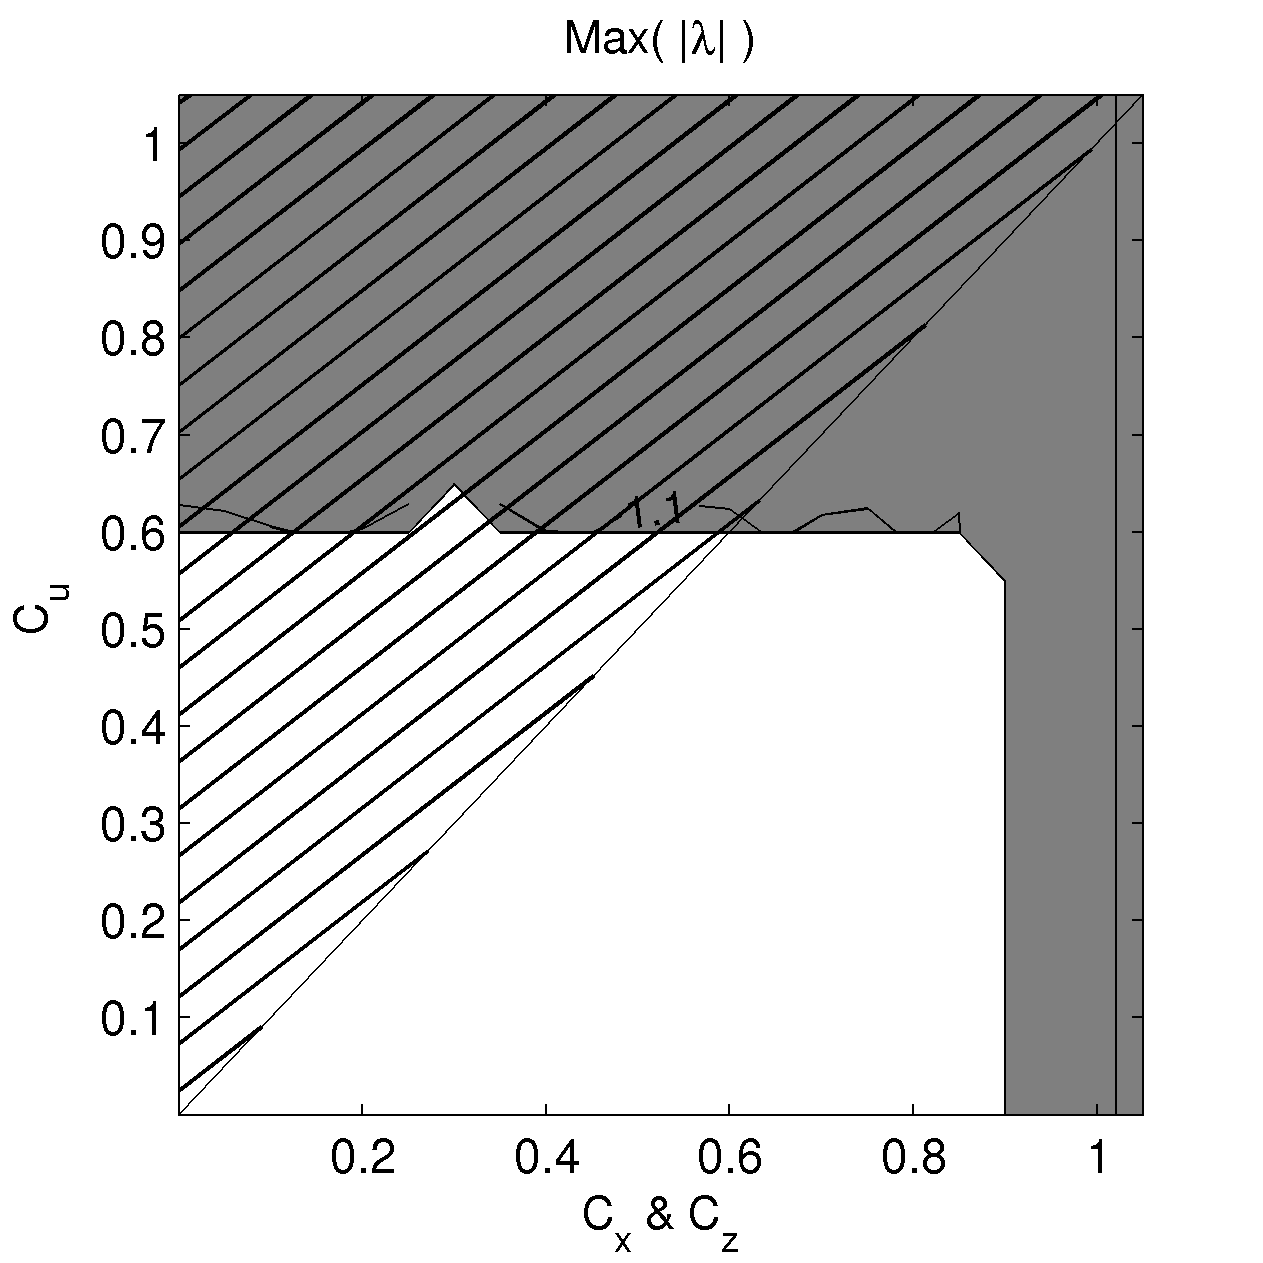
\includegraphics[width=.4\textwidth]{FIGURES/stabadvlambdaimp10_cpl2.png}}
%   \caption{Amplitude of the largest eigenvalue as a function of $C_x\ =\ C_z$ and $C_u$.\\
%       Unstable area ($\mid\lambda\mid >1$) is in grey.\\
%       Hatched area: $C_u > C_x$ \\
%       (a): $N_f = 2$. (b): $N_f = 10$.\\
%       (a) and (b): implicit FB scheme with $\lambda_s = 0.1\ m^2/s$.}
%   \label{Figstabplotadv}
%\end{figure}

\begin{figure}[!ht]
   \centering
   \subfloat[][]{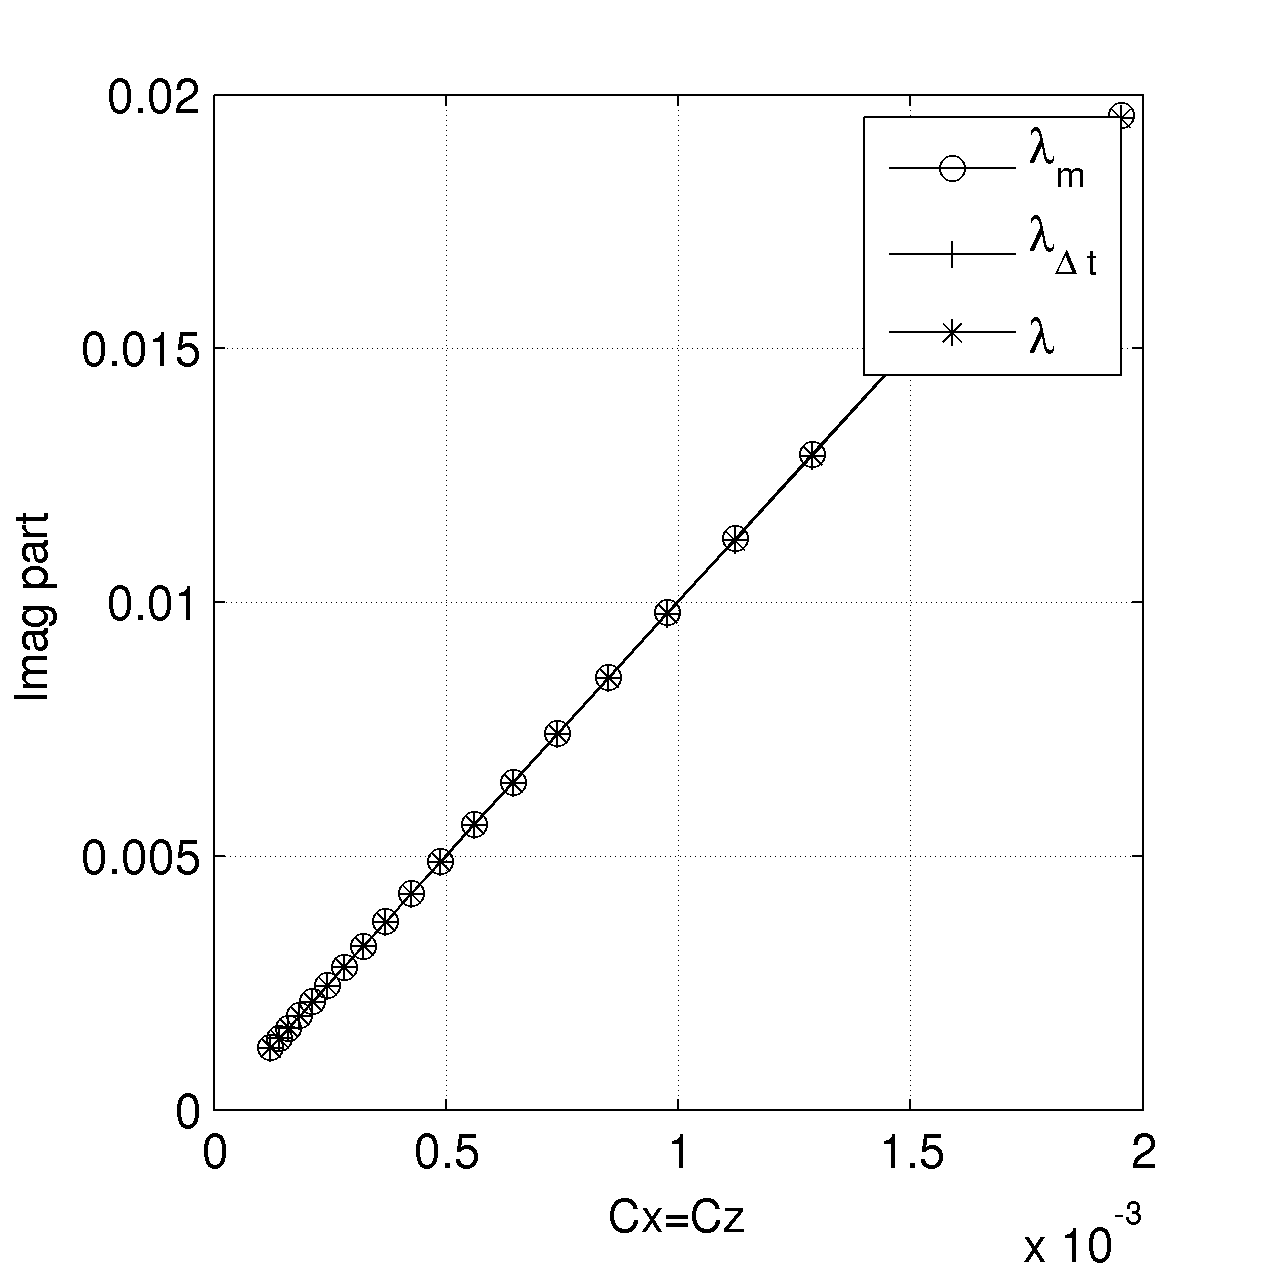
\includegraphics[width=.4\textwidth]{FIGURES/lambdai1_plot.png}}\quad
   \subfloat[][]{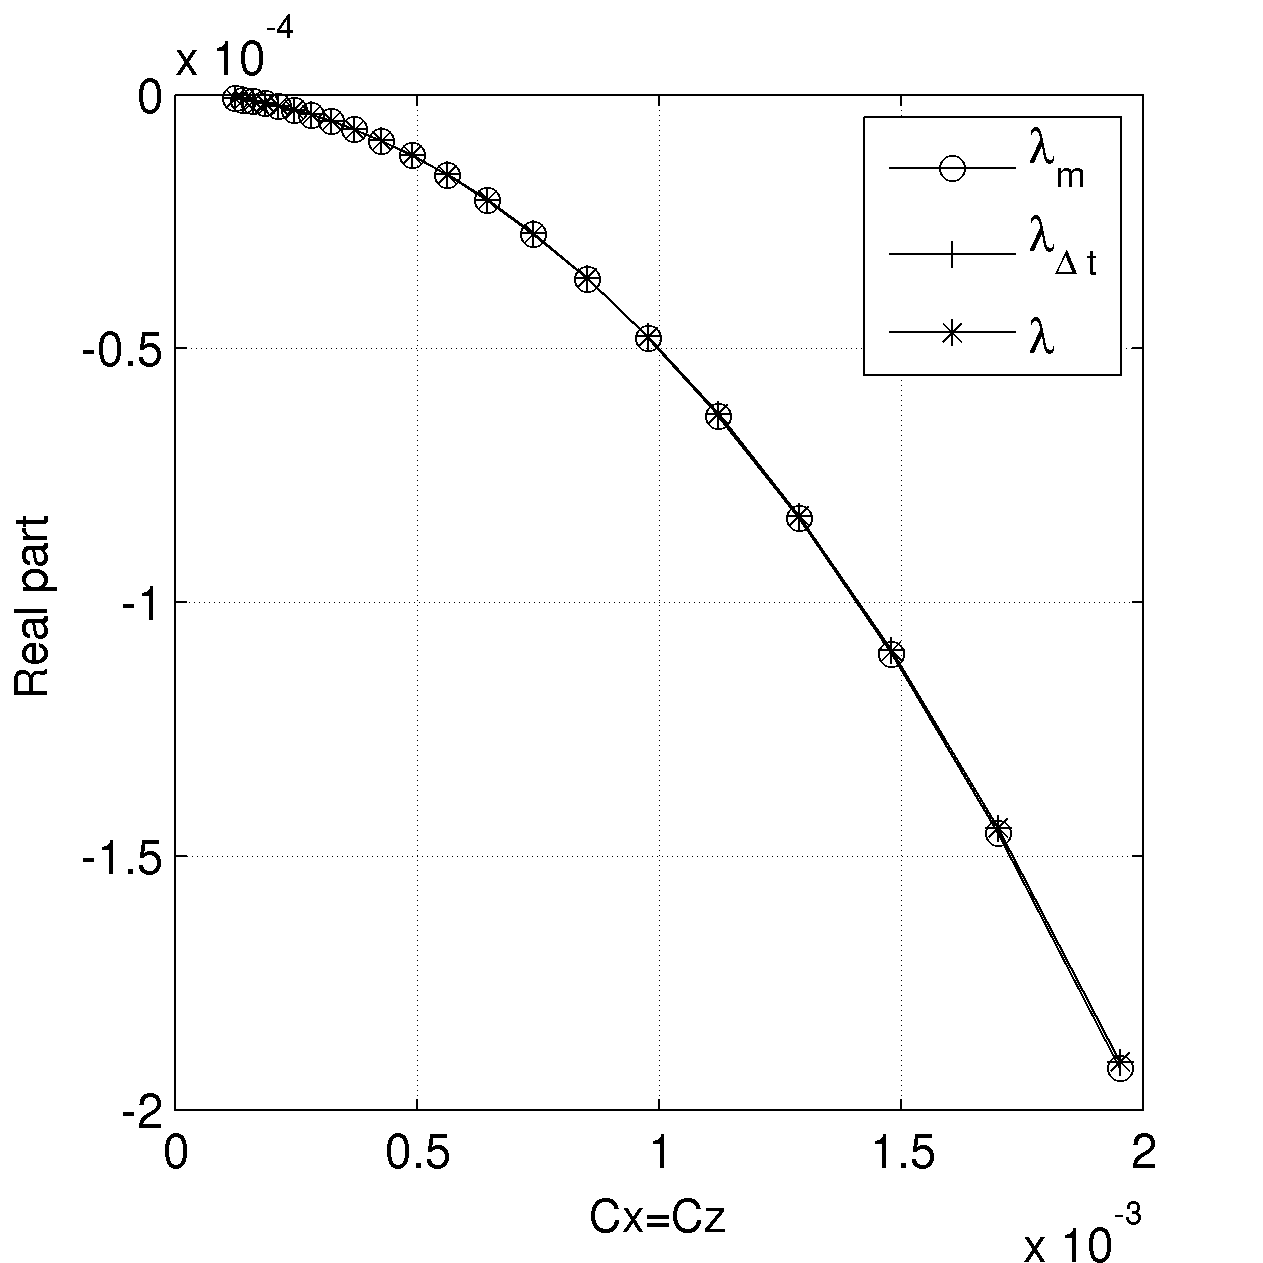
\includegraphics[width=.4\textwidth]{FIGURES/lambdar1_plot.png}}\\
   \subfloat[][]{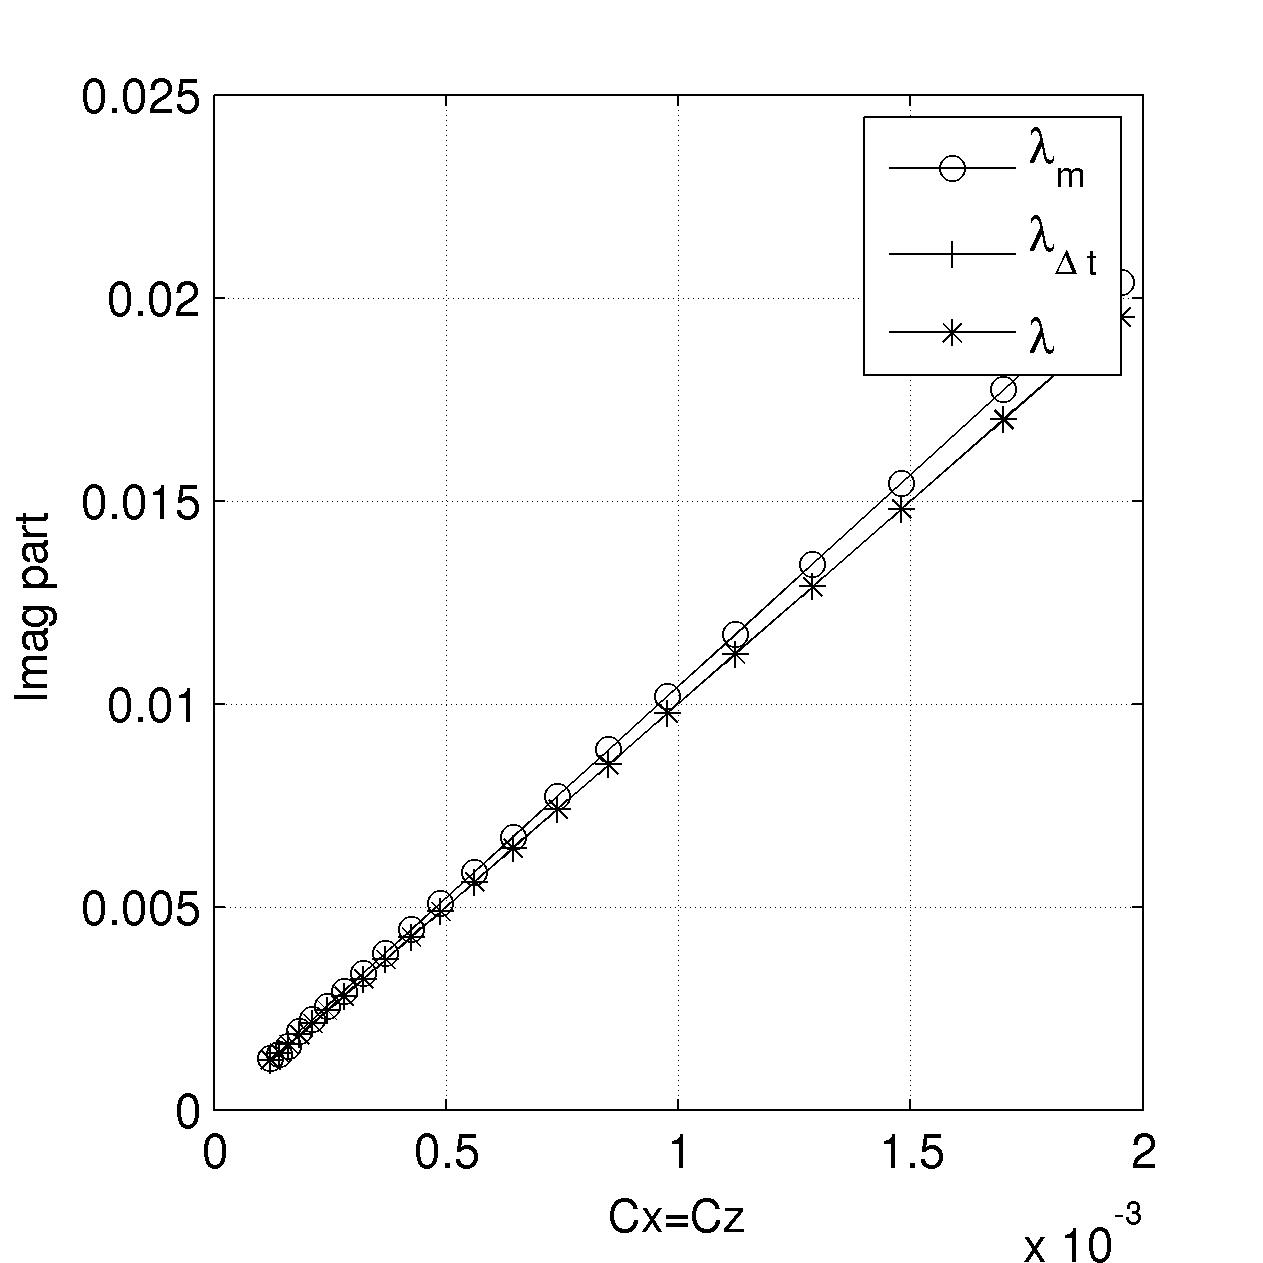
\includegraphics[width=.4\textwidth]{FIGURES/lambdai2_plot.png}}\quad
   \subfloat[][]{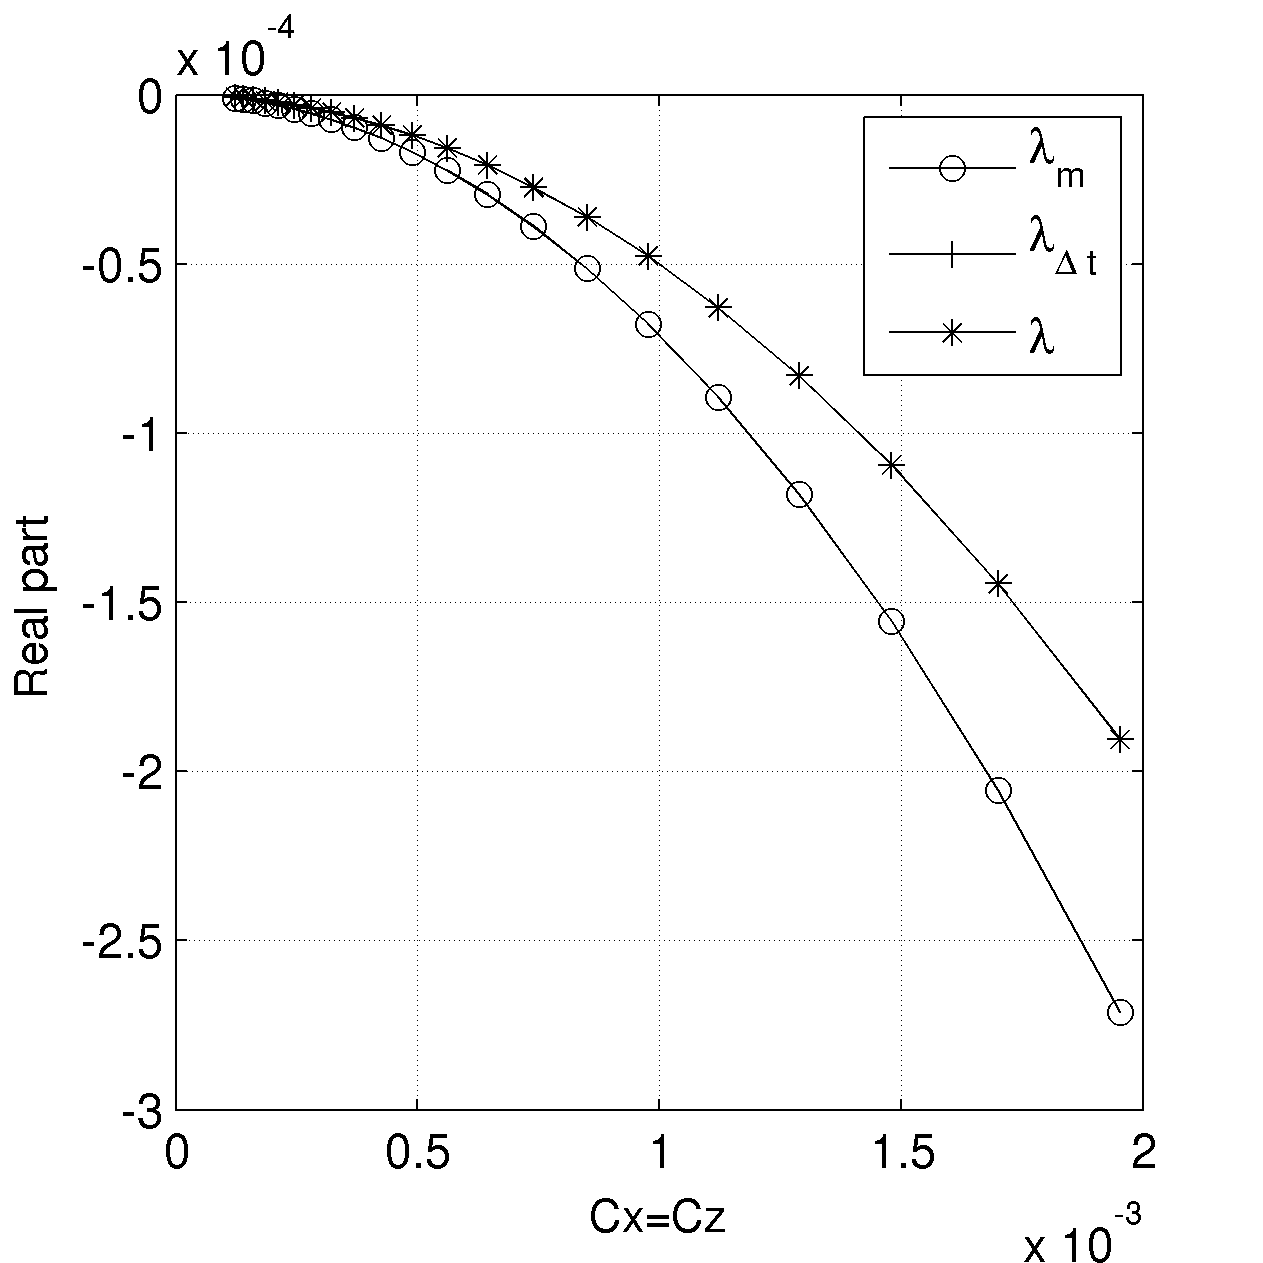
\includegraphics[width=.4\textwidth]{FIGURES/lambdar2_plot.png}}\\
   \subfloat[][]{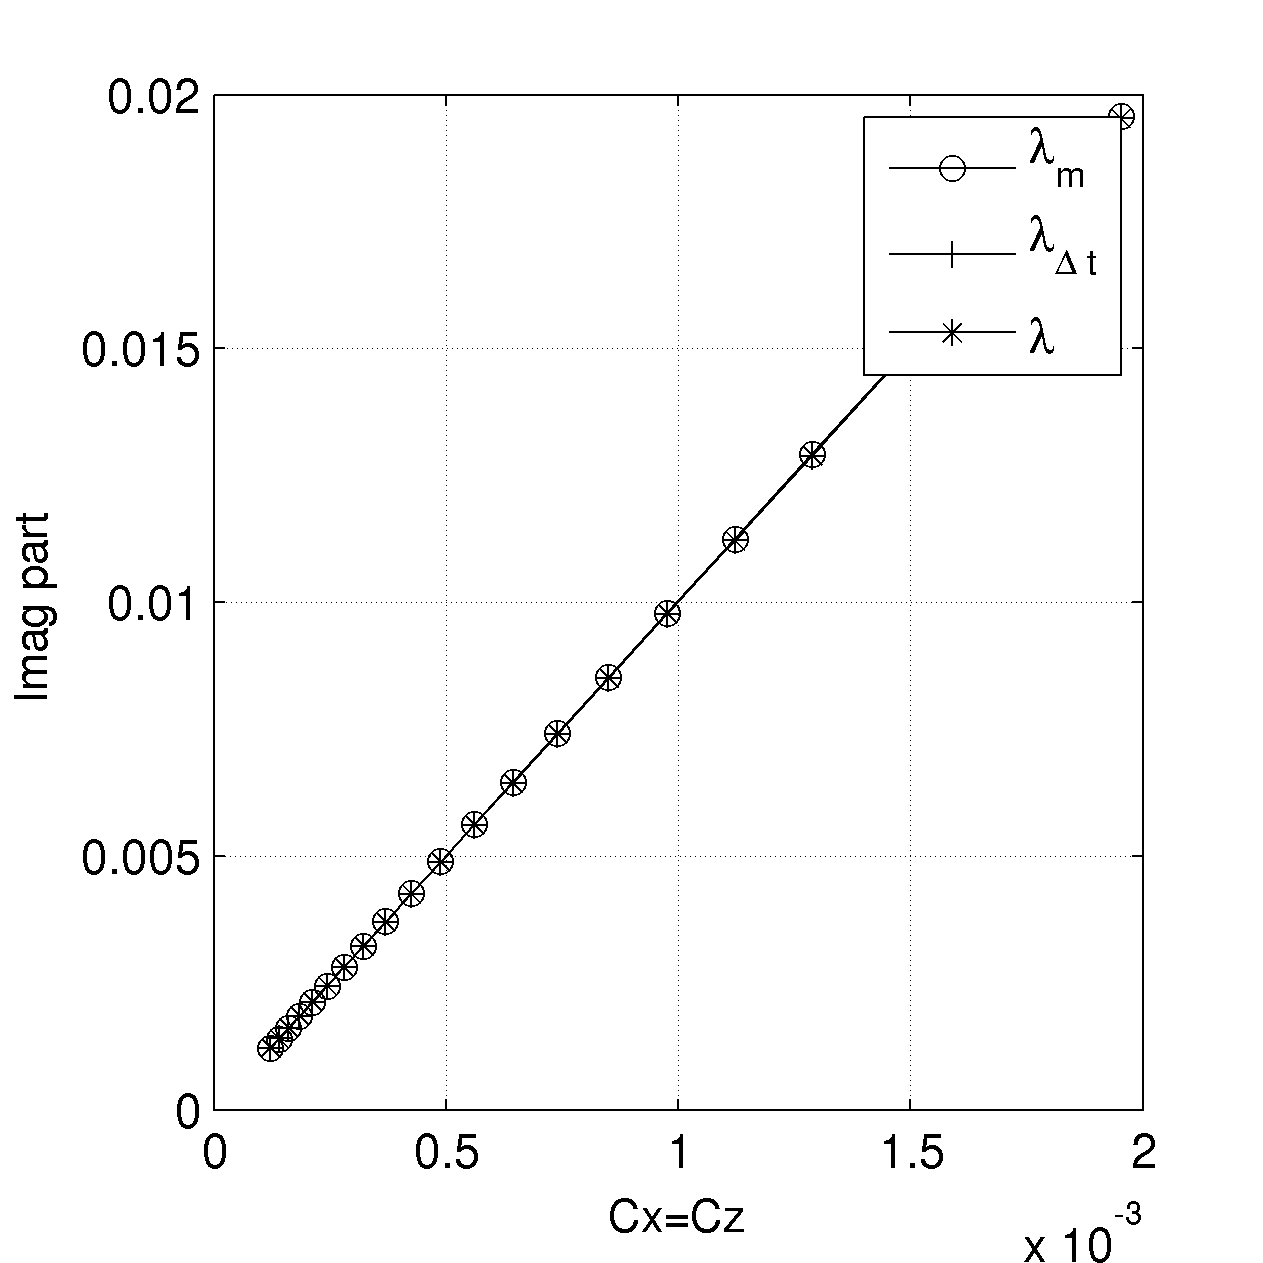
\includegraphics[width=.4\textwidth]{FIGURES/lambdai3_plot.png}}\quad
   \subfloat[][]{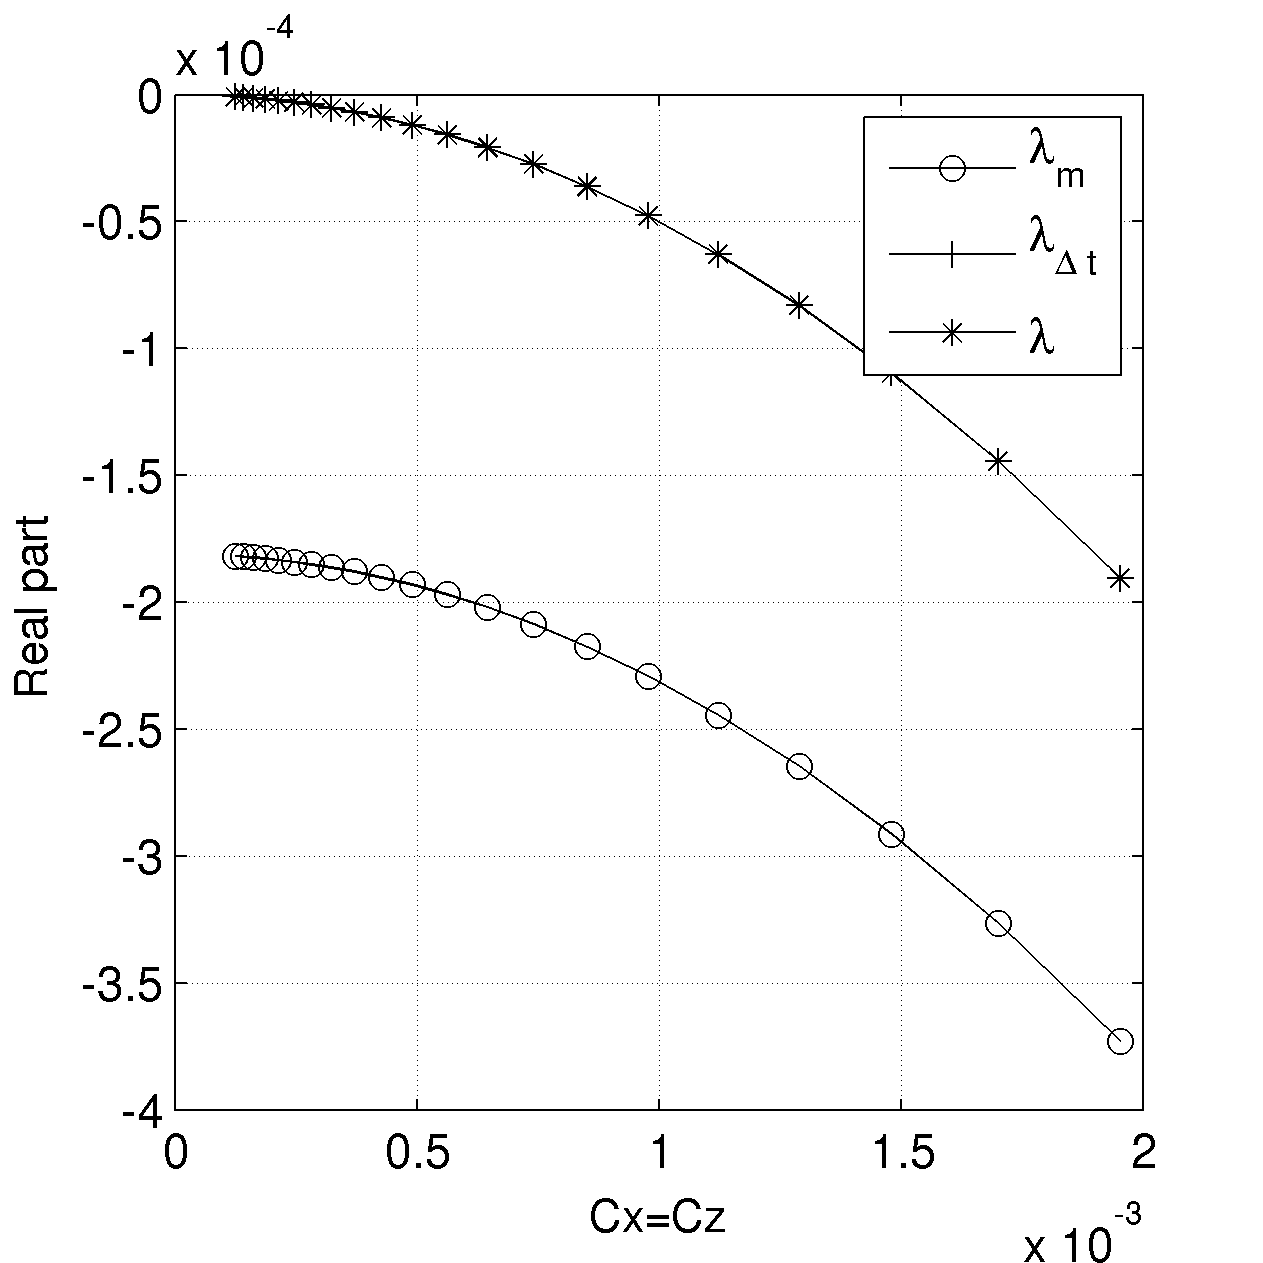
\includegraphics[width=.4\textwidth]{FIGURES/lambdar3_plot.png}}
   \caption{Acoustic waves: evolution of real (left) and imaginary (right) parts of $\lambda$, $\lambda_{\Delta t}$ and $\lambda$ with 
            Courant numbers ($Cx$ = $Cz$).\\
            (a) and (b): fast-mode only .
            (c) and (d): slow and fast modes ($N_f= 10$).
            (e) and (f): fast-mode only with second viscosity filtering.}
   \label{FigLambdaacous}
\end{figure}

\begin{figure}[!ht]
   \centering
   \subfloat[][]{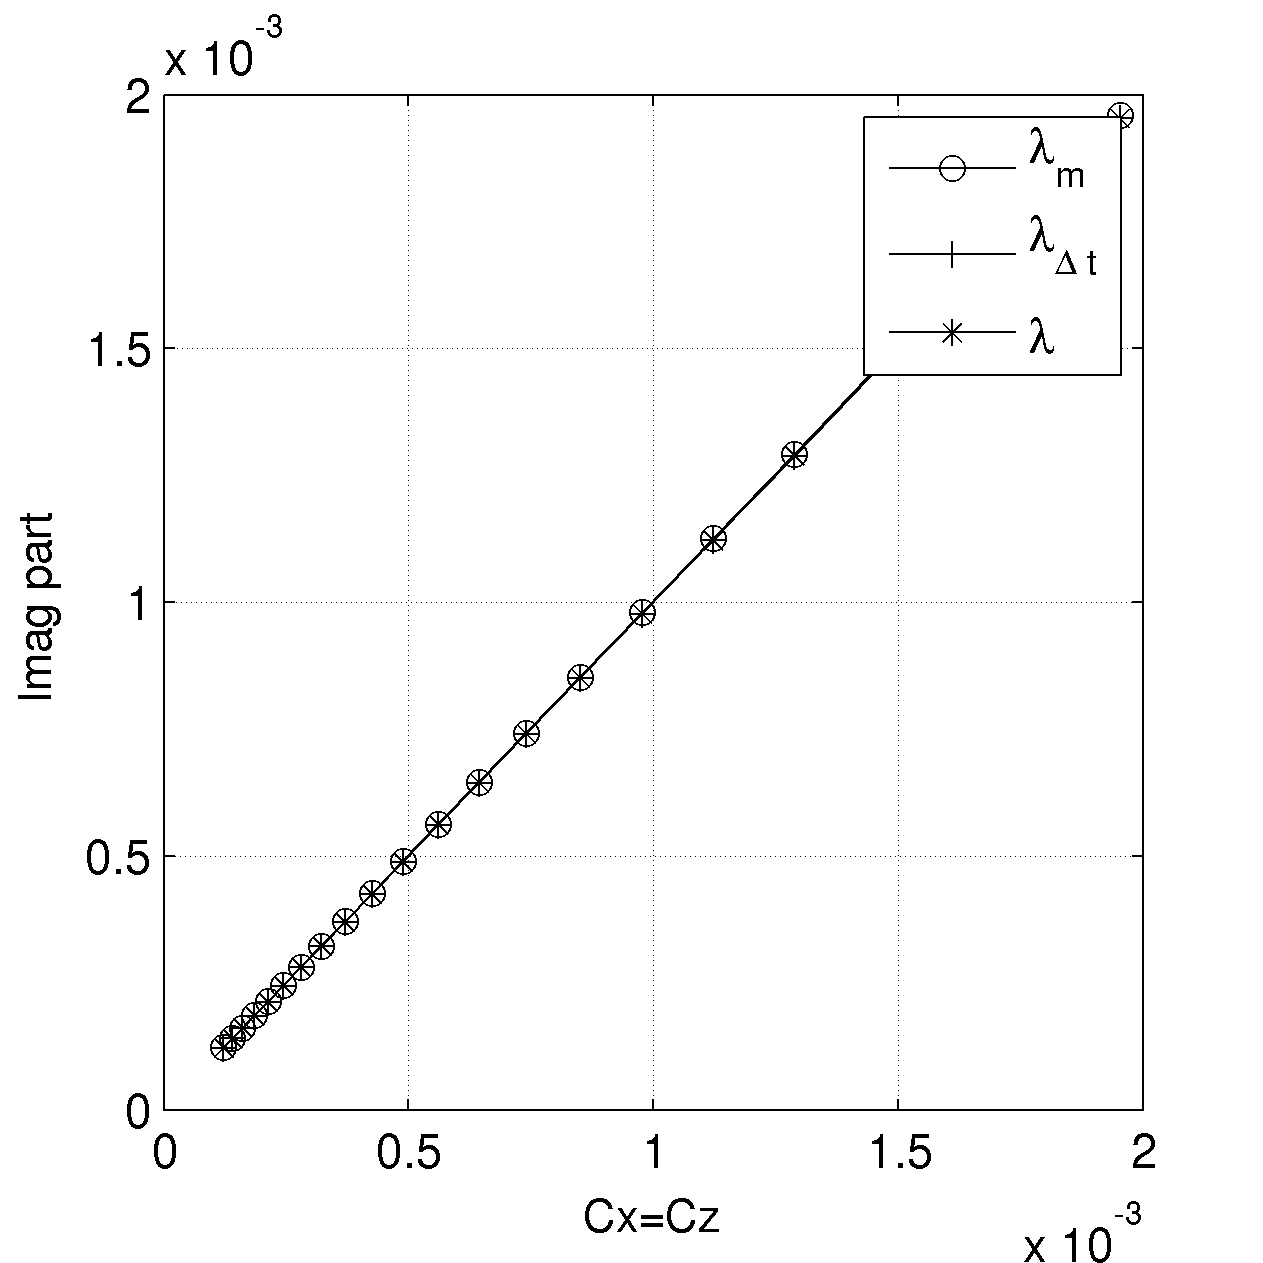
\includegraphics[width=.4\textwidth]{FIGURES/lambdai4_plot.png}}\quad
   \subfloat[][]{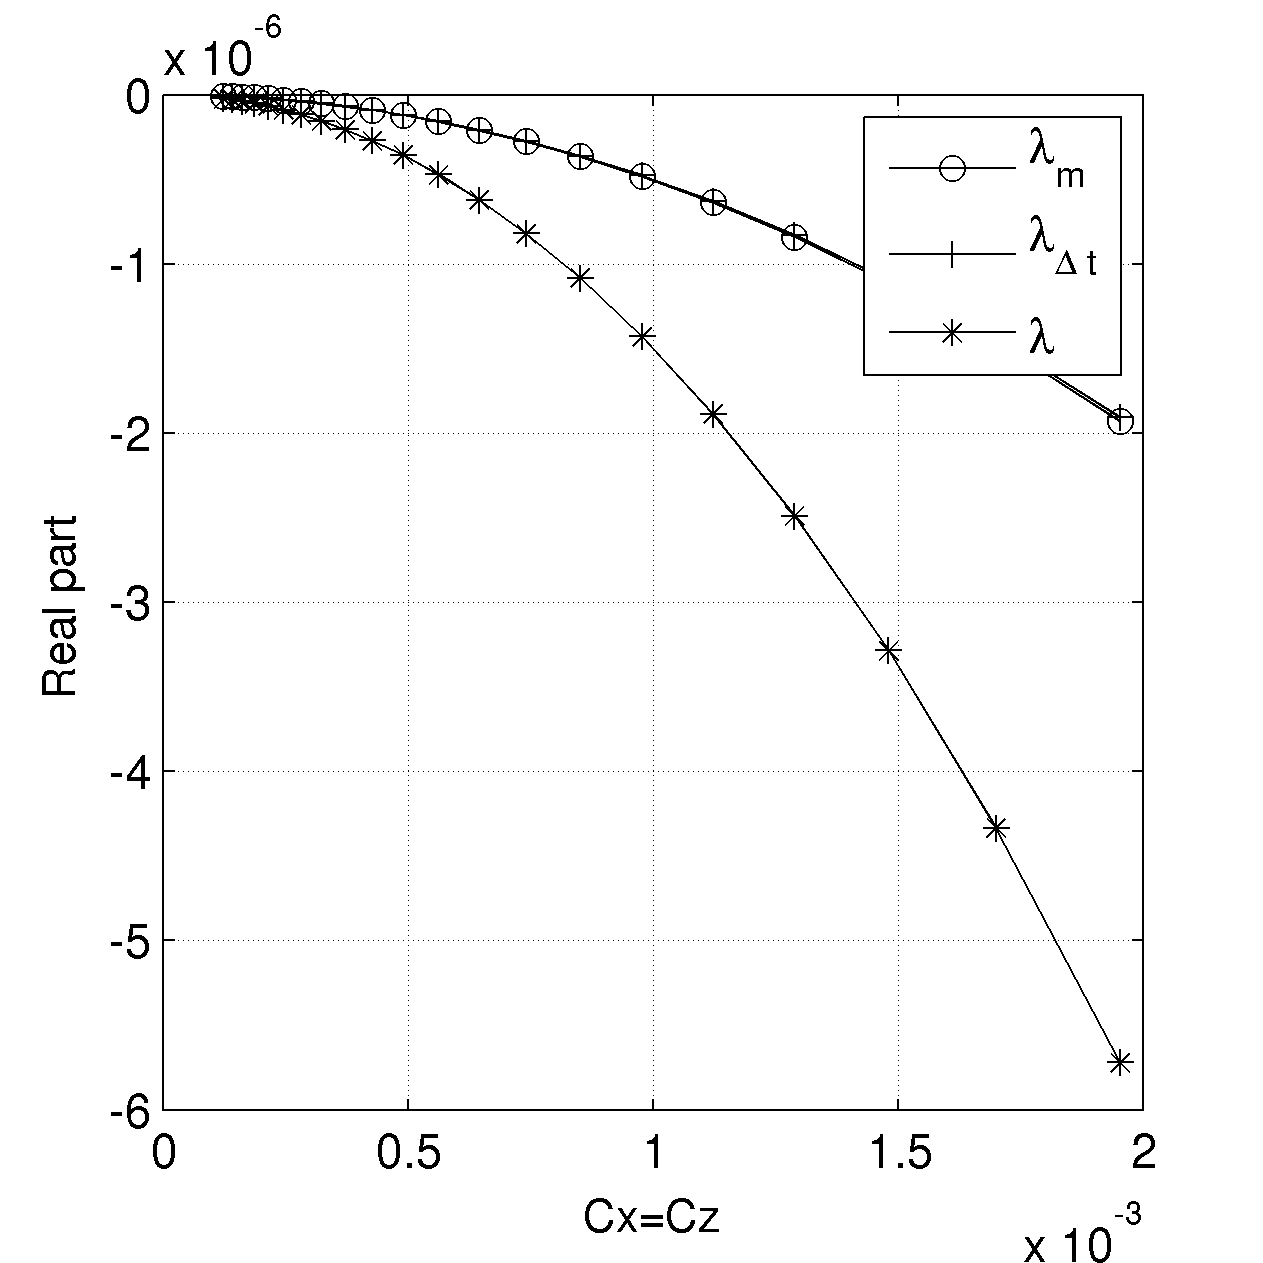
\includegraphics[width=.4\textwidth]{FIGURES/lambdar4_plot.png}}
   \caption{Acoustic waves: evolution of real (a) and imaginary (b) parts of $\lambda$, $\lambda_{\Delta t}$ and $\lambda$ with 
            Courant numbers ($Cx$ = $Cz$).}
   \label{FigLambdaacous2}
\end{figure}

\begin{figure}[!ht]
   \centering
   \subfloat[][]{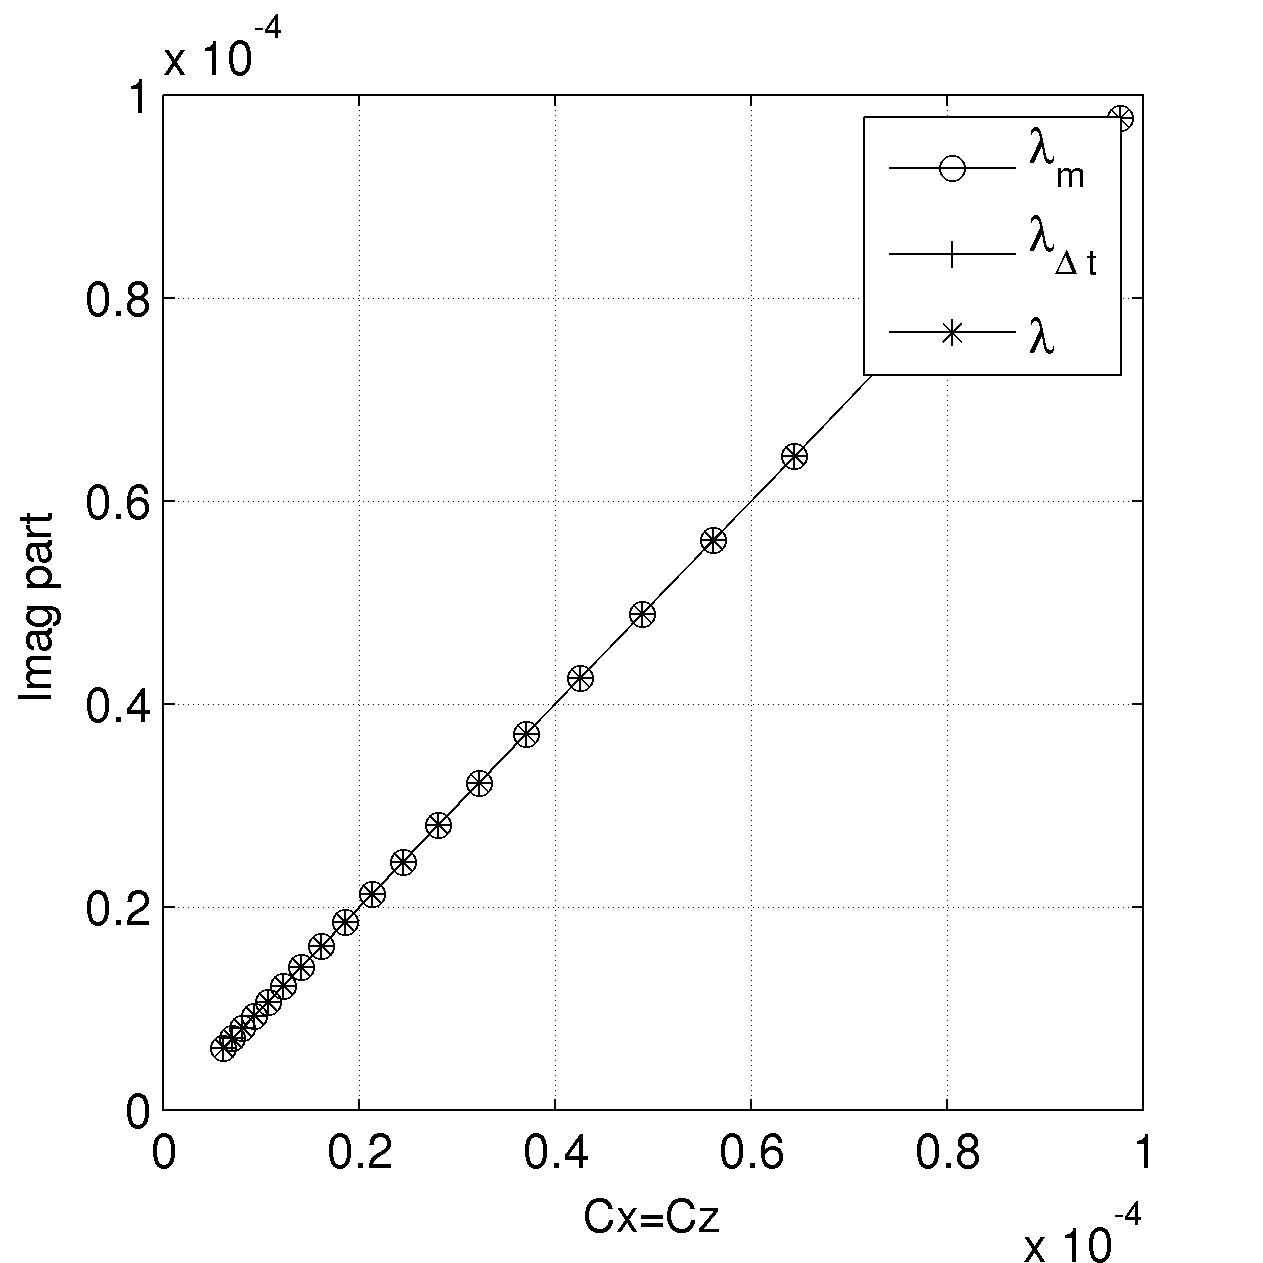
\includegraphics[width=.4\textwidth]{FIGURES/lambdaiS_plot.png}}\quad
   \subfloat[][]{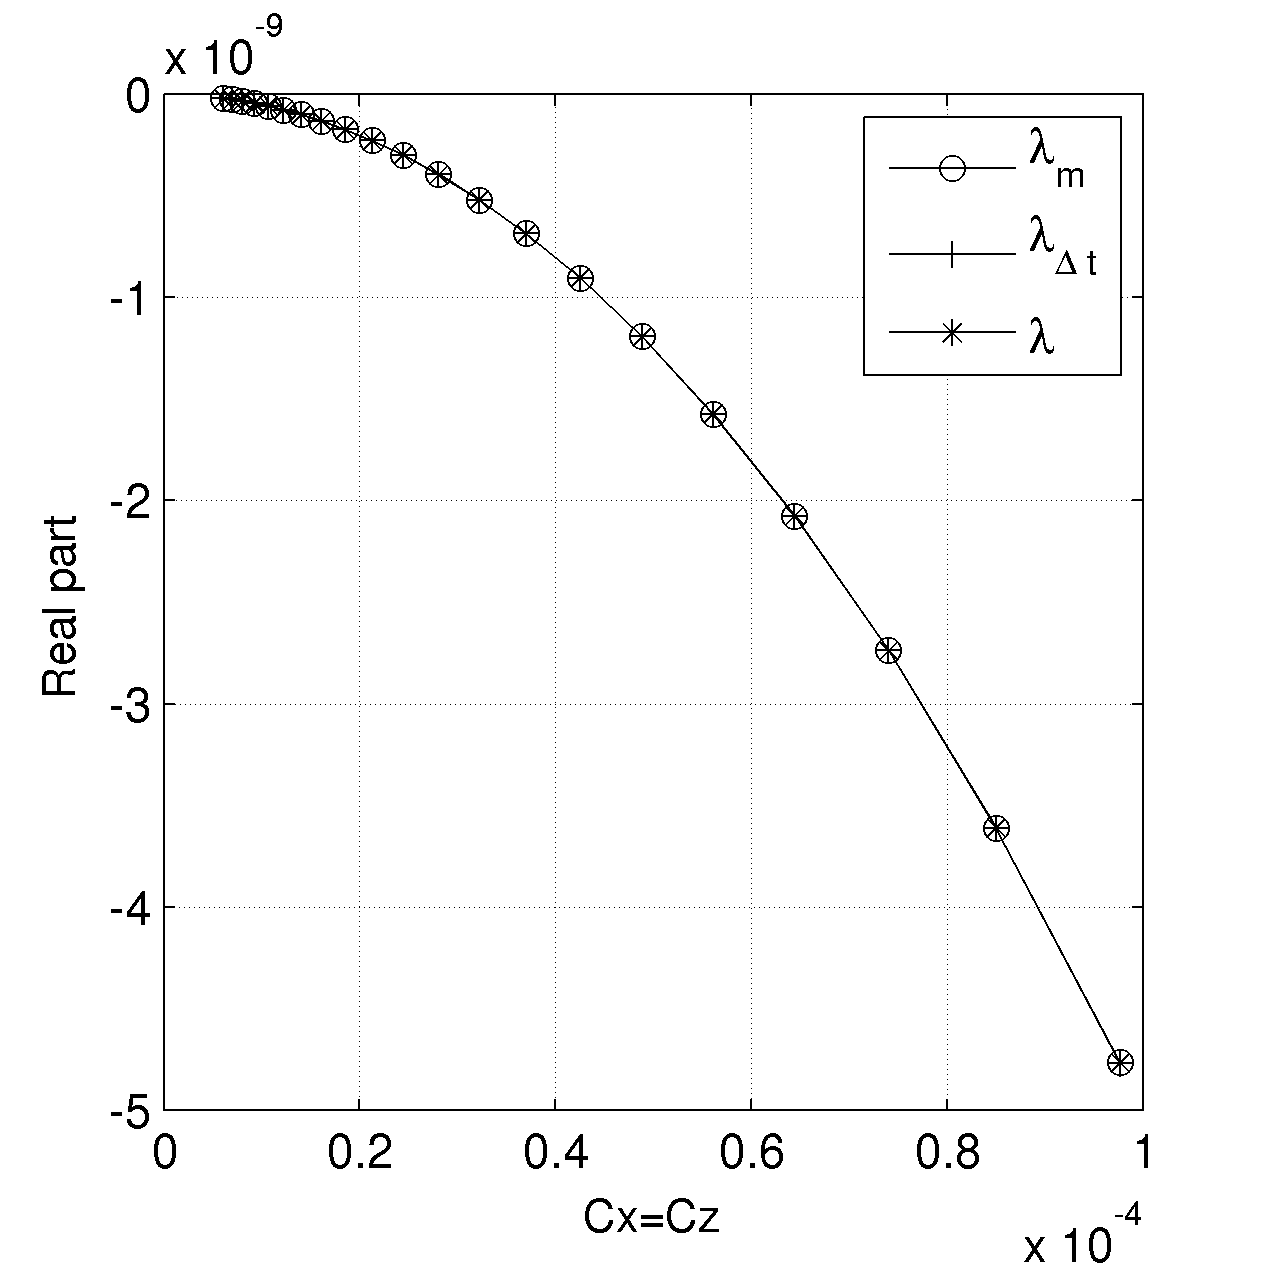
\includegraphics[width=.4\textwidth]{FIGURES/lambdarS_plot.png}}
   \caption{Acoustic-surface gravity waves: evolution of real (a) and imaginary (b) parts of$\lambda$, $\lambda_{\Delta t}$ and $\lambda$ with 
            Courant numbers ($Cx$ = $Cz$).}
   \label{FigLambdagravs}
\end{figure}

\begin{figure}[!ht]
   \centering
   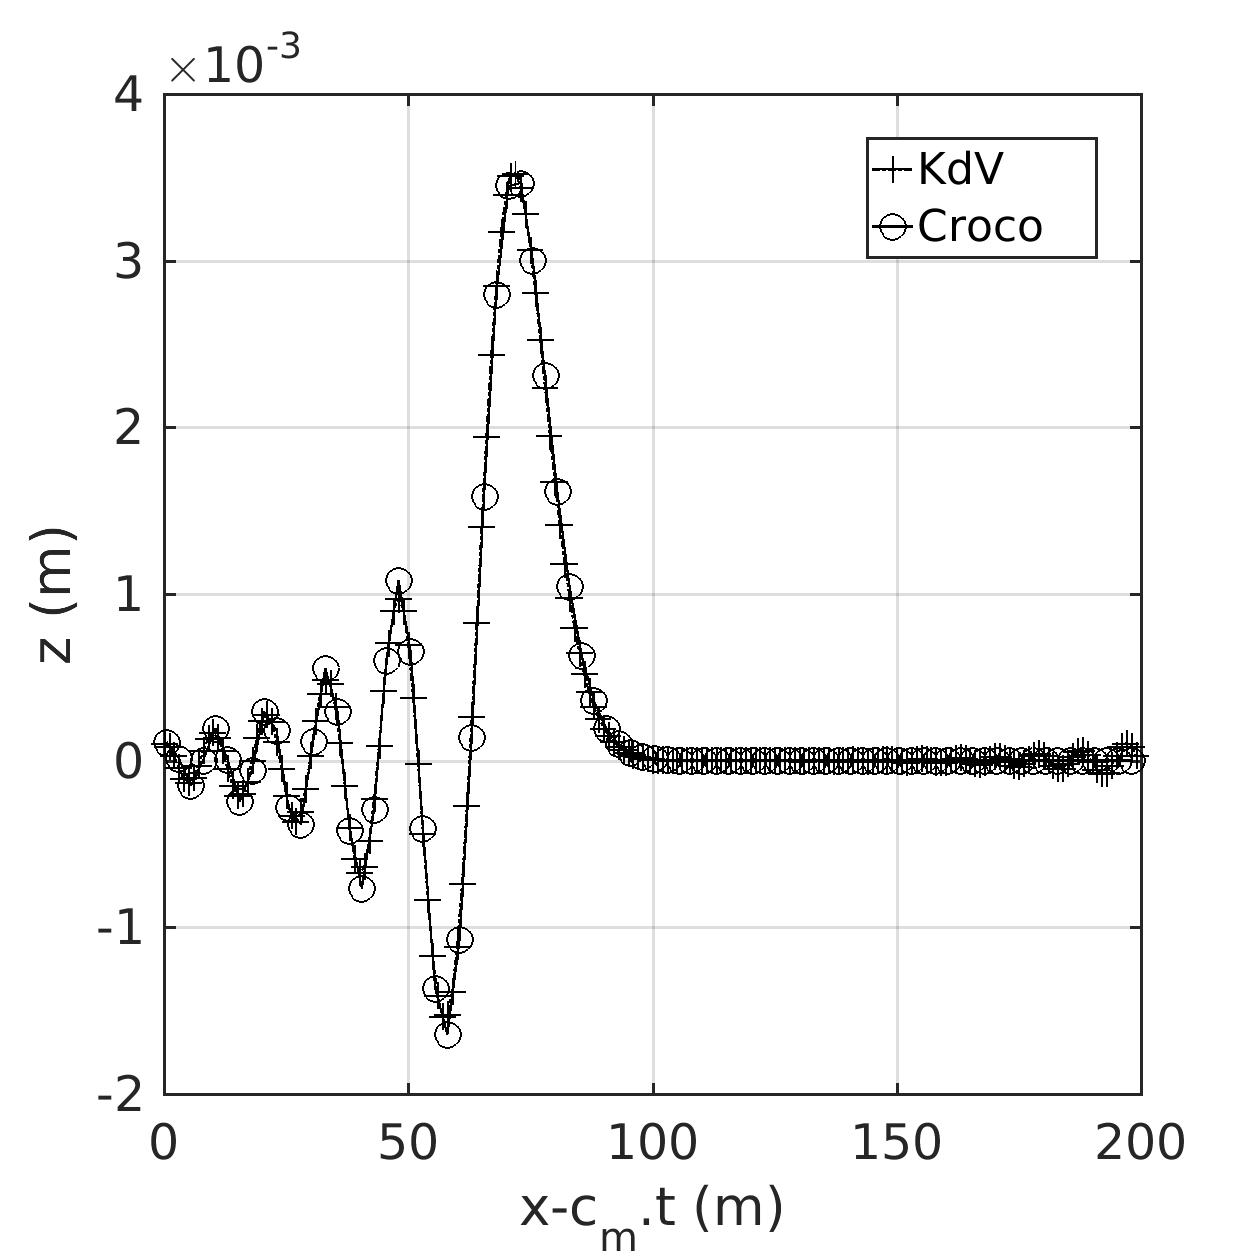
\includegraphics[width=.4\textwidth]{FIGURES/kdv_plot.png}
   \caption{Comparison of Croco and KdV equation.}
   \label{KdV}
\end{figure}

\newpage

 
\newpage
%%%%%%%%%%%%%%%%%%%%%%%%%%%%%%%%%%%%%%%%%%%%%%%%%%%%%%%%%%%%%%%%%%%%%%%%%%%%%
\section{Discussion, conclusions}
%%%%%%%%%%%%%%%%%%%%%%%%%%%%%%%%%%%%%%%%%%%%%%%%%%%%%%%%%%%%%%%%%%%%%%%%%%%%%
 \begin{itemize}[font=\small] 
  \item 
 \end{itemize}
 
\newpage


%%%%%%%%%%%%%%%%%%%%%%%%%%%%%%%%%%%%%%%%%%%%%%%%%%%%%%%%%%%%%%%%%%%%%%%%%%%%%
%\bibliography{paper_NBQ_1}
%%%%%%%%%%%%%%%%%%%%%%%%%%%%%%%%%%%%%%%%%%%%%%%%%%%%%%%%%%%%%%%%%%%%%%%%%%%%%
\end{document}
